%% LyX 2.0.6 created this file.  For more info, see http://www.lyx.org/.
%% Do not edit unless you really know what you are doing.
\documentclass[brazil]{article}
\usepackage[T1]{fontenc}
\usepackage[utf8]{inputenc}
\usepackage{geometry}
\geometry{verbose,tmargin=2cm,bmargin=3cm,lmargin=2.5cm,rmargin=2.5cm}
\usepackage{hyperref}
\usepackage{fancybox}
\usepackage{calc}
\usepackage{units}
\usepackage{amsmath}
\usepackage{amssymb}
\usepackage{esint}
\usepackage{babel}
\usepackage{natbib}
\usepackage[colorinlistoftodos]{todonotes}  % pacore para inserir comentários
\usepackage{verbatim}
\usepackage{booktabs}
\usepackage{graphicx}
\usepackage{caption}
\usepackage{tikz}
\usepackage{subcaption}
\usepackage{setspace}
\usepackage{fancyhdr}
\usepackage{float}
\usepackage{xcolor}
\usepackage[siunitx]{circuitikz} % Para colocar desenho de circuitos
\usepackage{multirow} % Para colocar celulas aglutinadas em tabelas
\usepackage{pgfplots} % Para fazer gráficos
\usepackage{framed} % Para fazer boxes


%\usepackage{tikz}

\usetikzlibrary{arrows, calc, decorations.markings, positioning}

%\pagestyle{empty}

\makeatletter
\newenvironment{timeline}[6]{%
    % #1 is startyear
    % #2 is tlendyear
    % #3 is yearcolumnwidth
    % #4 is rulecolumnwidth
    % #5 is entrycolumnwidth
    % #6 is timelineheight

    \newcommand{\startyear}{#1}
    \newcommand{\tlendyear}{#2}

    \newcommand{\yearcolumnwidth}{#3}
    \newcommand{\rulecolumnwidth}{#4}
    \newcommand{\entrycolumnwidth}{#5}
    \newcommand{\timelineheight}{#6}

    \newcommand{\templength}{}

    \newcommand{\entrycounter}{0}

    % http://tex.stackexchange.com/questions/85528/checking-whether-or-not-a-node-has-been-previously-defined
    % http://tex.stackexchange.com/questions/37709/how-can-i-know-if-a-node-is-already-defined
    \long\def\ifnodedefined##1##2##3{%
        \@ifundefined{pgf@sh@ns@##1}{##3}{##2}%
    }

    \newcommand{\ifnodeundefined}[2]{%
        \ifnodedefined{##1}{}{##2}
    }

    \newcommand{\drawtimeline}{%
        \draw[timelinerule] (\yearcolumnwidth+5pt, 0pt) -- (\yearcolumnwidth+5pt, -\timelineheight);
        \draw (\yearcolumnwidth+0pt, -10pt) -- (\yearcolumnwidth+10pt, -10pt);
        \draw (\yearcolumnwidth+0pt, -\timelineheight+15pt) -- (\yearcolumnwidth+10pt, -\timelineheight+15pt);

        \pgfmathsetlengthmacro{\templength}{neg(add(multiply(subtract(\startyear, \startyear), divide(subtract(\timelineheight, 25), subtract(\tlendyear, \startyear))), 10))}
        \node[year] (year-\startyear) at (\yearcolumnwidth, \templength) {\startyear};

        \pgfmathsetlengthmacro{\templength}{neg(add(multiply(subtract(\tlendyear, \startyear), divide(subtract(\timelineheight, 25), subtract(\tlendyear, \startyear))), 10))}
        \node[year] (year-\tlendyear) at (\yearcolumnwidth, \templength) {\tlendyear};
    }

    \newcommand{\entry}[2]{%
        % #1 is the year
        % #2 is the entry text

        \pgfmathtruncatemacro{\lastentrycount}{\entrycounter}
        \pgfmathtruncatemacro{\entrycounter}{\entrycounter + 1}

        \ifdim \lastentrycount pt > 0 pt%
            \node[entry] (entry-\entrycounter) [below of=entry-\lastentrycount] {##2};
        \else%
            \pgfmathsetlengthmacro{\templength}{neg(add(multiply(subtract(\startyear, \startyear), divide(subtract(\timelineheight, 25), subtract(\tlendyear, \startyear))), 10))}
            \node[entry] (entry-\entrycounter) at (\yearcolumnwidth+\rulecolumnwidth+10pt, \templength) {##2};
        \fi

        \ifnodeundefined{year-##1}{%
            \pgfmathsetlengthmacro{\templength}{neg(add(multiply(subtract(##1, \startyear), divide(subtract(\timelineheight, 25), subtract(\tlendyear, \startyear))), 10))}
            \draw (\yearcolumnwidth+2.5pt, \templength) -- (\yearcolumnwidth+7.5pt, \templength);
            \node[year] (year-##1) at (\yearcolumnwidth, \templength) {##1};
        }

        \draw ($(year-##1.east)+(2.5pt, 0pt)$) -- ($(year-##1.east)+(7.5pt, 0pt)$) -- ($(entry-\entrycounter.west)-(5pt,0)$) -- (entry-\entrycounter.west);
    }

    \newcommand{\plainentry}[2]{% plainentry won't print date in the timeline
        % #1 is the year
        % #2 is the entry text

        \pgfmathtruncatemacro{\lastentrycount}{\entrycounter}
        \pgfmathtruncatemacro{\entrycounter}{\entrycounter + 1}

        \ifdim \lastentrycount pt > 0 pt%
            \node[entry] (entry-\entrycounter) [below of=entry-\lastentrycount] {##2};
        \else%
            \pgfmathsetlengthmacro{\templength}{neg(add(multiply(subtract(\startyear, \startyear), divide(subtract(\timelineheight, 25), subtract(\tlendyear, \startyear))), 10))}
            \node[entry] (entry-\entrycounter) at (\yearcolumnwidth+\rulecolumnwidth+10pt, \templength) {##2};
        \fi

        \ifnodeundefined{invisible-year-##1}{%
            \pgfmathsetlengthmacro{\templength}{neg(add(multiply(subtract(##1, \startyear), divide(subtract(\timelineheight, 25), subtract(\tlendyear, \startyear))), 10))}
            \draw (\yearcolumnwidth+2.5pt, \templength) -- (\yearcolumnwidth+7.5pt, \templength);
            \node[year] (invisible-year-##1) at (\yearcolumnwidth, \templength) {};
        }

        \draw ($(invisible-year-##1.east)+(2.5pt, 0pt)$) -- ($(invisible-year-##1.east)+(7.5pt, 0pt)$) -- ($(entry-\entrycounter.west)-(5pt,0)$) -- (entry-\entrycounter.west);
    }

    \begin{tikzpicture}
        \tikzstyle{entry} = [%
            align=left,%
            text width=\entrycolumnwidth,%
            node distance=10mm,%
            anchor=west]
        \tikzstyle{year} = [anchor=east]
        \tikzstyle{timelinerule} = [%
            draw,%
            decoration={markings, mark=at position 1 with {\arrow[scale=1.5]{latex'}}},%
            postaction={decorate},%
            shorten >=0.4pt]

        \drawtimeline
}
{
    \end{tikzpicture}
    \let\startyear\@undefined
    \let\tlendyear\@undefined
    \let\yearcolumnwidth\@undefined
    \let\rulecolumnwidth\@undefined
    \let\entrycolumnwidth\@undefined
    \let\timelineheight\@undefined
    \let\entrycounter\@undefined
    \let\ifnodedefined\@undefined
    \let\ifnodeundefined\@undefined
    \let\drawtimeline\@undefined
    \let\entry\@undefined
}
\pagestyle{fancy}

\graphicspath{ {anexos/} }

% Para fazer a timeline
% http://tex.stackexchange.com/questions/196794/how-can-you-create-a-vertical-timeline
\newcommand\ytl[2]{
\parbox[b]{8em}{\hfill{\color{cyan}\bfseries\sffamily #1}~$\cdots\cdots$~}\makebox[0pt][c]{$\bullet$}\vrule\quad \parbox[c]{8.5cm}{\vspace{7pt}\color{red!40!black!80}\raggedright\sffamily #2.\\[7pt]}\\[-3pt]}


\usepackage{tcolorbox} % Implementar highlights
\newtcbox{\hl}[1][yellow]{on line, arc=7pt,colback=#1!10!white,colframe=#1!50!black,
  before upper={\rule[-3pt]{0pt}{10pt}},boxrule=1pt, boxsep=0pt,left=6pt,
  right=6pt,top=2pt,bottom=2pt}

\begin{document}

\begin{titlepage}

\newcommand{\HRule}{\rule{\linewidth}{0.5mm}} % Defines a new command for the horizontal lines, change thickness here
%\theoremstyle{definition}
\newtheorem{exemplo}{Exemplo}[section]


\center % Center everything on the page
 
%----------------------------------------------------------------------------------------
%   HEADING SECTIONS
%----------------------------------------------------------------------------------------

\textsc{\LARGE Pontifícia Universidade Católica do Rio de Janeiro}\\[1.5cm] % Name of your university/college
\textsc{\Large Disciplina de Economia da Energia Elétrica}\\[0.5cm] % Major heading such as course name
%\textsc{\large Minor Heading}\\[0.5cm] % Minor heading such as course title

%----------------------------------------------------------------------------------------
%   TITLE SECTION
%----------------------------------------------------------------------------------------

\HRule \\[0.4cm]
{ \huge \bfseries Apostila da disciplina}\\[0.4cm] % Title of your document
\HRule \\[1.5cm]
 
%----------------------------------------------------------------------------------------
%   AUTHOR SECTION
%----------------------------------------------------------------------------------------

\begin{minipage}{0.4\textwidth}
\begin{flushleft} \large
\emph{Autores:}\\
Gabriel Filipe Rodrigues Vasconcelos \thanks{email: gabrielrvsc@yahoo.com.br}\\
        Lívia Ferreira Rodrigues \thanks{email: liviaferrodrigues@gmail.com}\\
        Marcelo Castiel Ruas\thanks{email: mcruas@gmail.com}\\

\end{flushleft}
\end{minipage}
~
\begin{minipage}{0.4\textwidth}
\begin{flushright} \large
\emph{Professores:} \\
Alexandre Street\\
Delberis Lima\\
Luiz Augusto Barroso
\end{flushright}
\end{minipage}\\[2cm]

% If you don't want a supervisor, uncomment the two lines below and remove the section above
%\Large \emph{Author:}\\
%John \textsc{Smith}\\[3cm] % Your name

%----------------------------------------------------------------------------------------
%   DATE SECTION
%----------------------------------------------------------------------------------------

{\large \today}\\[2cm] % Date, change the \today to a set date if you want to be precise

%----------------------------------------------------------------------------------------
%   LOGO SECTION
%----------------------------------------------------------------------------------------


\includegraphics{logo.png}\\[1cm] % Include a department/university logo - this will require the graphicx package
 
%----------------------------------------------------------------------------------------

\vfill % Fill the rest of the page with whitespace

\end{titlepage}



%\doublespace

%\title{Trabalho final para a disciplina de Análise de Séries Temporais Financeiras}

%\author{Gabriel Filipe Rodrigues Vasconcelos \thanks{email: gabrielrvsc@yahoo.com.br}\\
 %       Lívia Ferreira Rodrigues \thanks{email: liviaferrodrigues@gmail.com}\\
  %      Marcelo Castiel Ruas\thanks{email: mcruas@gmail.com}\\
  %      Mariana Arozo Benício de Melo\thanks{email: mariarozo@gmail.com}}\\
  %      \textbf{Professor:} Cristiano A. Fernandes}
        
%\maketitle
\tableofcontents


%\section{Conceitos Básicos}

\subsection{Introdução}


% \subsection{Problema criação de um sistema}
Suponha que estamos num país em que não haja energia elétrica e desejamos
definir um plano de implantação para suprir a necessidade de energia
dos seus habitantes que pararam no século XIX. Para ser feita de forma eficiente, esta tarefa requer, de início, conhecimento acerca da demanda por energia dos habitantes e dos custos para atender esta demanda.

O primeiro passo é estimar qual é a demanda por energia nesse país.
Mas não basta um plano contendo apenas a demanda imediata; a expansão do sistema deve ser prevista preferencialmente com décadas de antecedência. E este é apenas o primeiro passo de uma série de etapas que compõe o planejamento de um sistema elétrico. As etapas são as seguintes: 
\begin{itemize}
\item Planejamento de capacidade
\item Definição dos custos de produção
\item Planejamento do estoque de recursos hídricos
\item Definição dos recursos a serem utilizados dadas as restrições
\item Despacho econômico (ou quanto a usina irá produzir de forma a minimizar os custos totais)
\item Fluxo de potência
\item Proteção e estabilidade do sistema
\end{itemize}

O diagrama apresentado na figura \ref{fig:Horizontes-de-planejamento} mostra as diferentes etapas relacionando com seus horizontes de planejamento, e seu nível de detalhamento. Nota-se que quanto menor o horizonte de tempo, maior deve ser o nível de detalhamento necessário para a correta operação. Por exemplo, não faz sentido discutir despacho econômico quando lidamos com projetos de instalação de novas usinas para aumento da capacidade.

\begin{figure}[h]
\begin{centering}
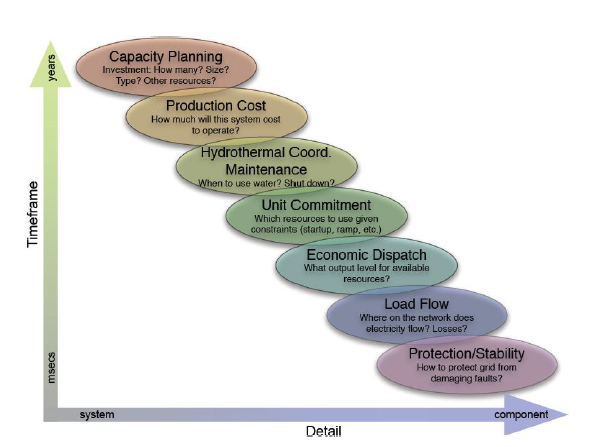
\includegraphics[scale=1]{anexos/hor-plan}
\par\end{centering}

\caption{\label{fig:Horizontes-de-planejamento}Horizontes de planejamento}
\end{figure}



Uma vez definida a demanda a atender, devemos escolher qual tipo de
usina implantar. Existem diversos tipos, como eólica, hidrelétrica,
nuclear, termelétrica (a gás, a carvão), entre outras. Além das diferenças
regionais entre a disponibilidade dos recursos naturais, há ainda
diferenças nas relações entre o custo de investimento inicial e o
custo de geração da energia. Por exemplo, uma usina termelétrica possui
geralmente um custo inicial menor que uma hidrelétrica, porém o custo
de geração da segunda é menor. A melhor solução a ser adotada possivelmente
passa pela utilização de uma combinação de diversos tipos, alguns
com custo de geração baixo mas altos investimentos iniciais para estarem
sempre ligados, e outros com baixos investimos iniciais mas alto custo
de geração para cobrir picos de demanda. Outras variáveis importantes,
além do custo das usinas, são a sazonalidade dos recursos e o tempo
de inicialização e desligamento de uma usina. O custo da operação do sistema de energia, incluindo todas suas restrições, também deve ser determinado. Para isso, é necessário realizar
o planejamento operacional, que observa horizontes menores e inclui,
por exemplo, o despacho econômico das usinas e a gestão de recursos
hídricos. 


Pode-se perceber que existem muitas variáveis envolvidas, custos desconhecidos,
e incertezas dos mais diversos tipos que afetam o funcionamento do
sistema, como a situação política do oriente médio ou até mesmo o
fenômeno El Niño. Considerar todas as variáveis ao mesmo tempo para
definir as quantidades ótimas, em qualquer estágio do planejamento,
requer um esforço computacional imenso, além de saber utilizar modelos estatísticos e utilizar métodos de mensuração de risco. Isso torna o estudo de métodos
de otimização um pré-requisito essencial para fazer uma boa gestão
de qualquer empresa que opera no mercado de energia.

Mas no que se consiste exatamente o mercado de energia?

% \subsection{Mecanismo de mercado}

Assim como no país fictício citado anteriormente, em todos os países a implantação inicial
da rede elétrica foi coordenada pela mesma instituição:
no caso, o governo. Isso mudou quando o Chile implantou o primeiro mercado de energia, em 1972, em que empresas vendiam a energia produzida por elas para as distribuidoras, por um preço determinado pelo mercado. Até então, todas as etapas do diagrama apresentado acima eram controladas pelo estado.
Assim, ao invés de ter um processo físico coordenando quanto cada empresa produz, é possível coordenar as quantidades fornecidas através da definição dos preços.
Caso os preços definidos sejam bem calibrados e não haja imperfeições
de mercado, é possível mostrar que as usinas fornecerão energia na
quantidade necessária, tal como uma empresa verticalmente integrada
faria dando ordens de produção para suas subsidiárias. Assim, estabelece-se
a fundamentação teórica para a criação de um mercado de energia.

Tal mercado tem vantagens e desvantagens. O mercado cria um ambiente competitivo e inovador que a longo e médio prazo pode conquistar avanços tecnológicos relevantes. Entretanto, um mercado mal formulado pode levar a uma competição desenfreada que pode levar ao não cumprimento de contratos e à falta de energia. 

Um exemplo interessante é o caso dos EUA e do Canadá, que possuem uma abordagem mista com relação à adoção de mercados de energia, em que cada estado ou província pode ou não adotar um esquema de mercado de energia. Na figura \ref{fig:mercado-eua}, está indicado em cores diferentes os diferentes mercados de energia existentes. Aqueles que possuem cores fracas não implementaram um mercado de energia, sendo o estado ou a província o responsável por fazer o planejamento e informar a quantidade produzida por cada produtor. Historicamente, nos EUA os mercados foram sendo implantados em alguns estados e passaram a ser adotados pelos estados vizinhos (um deles, o grupo Midwest ISO, conseguiu avançar para o Canadá, na província de Manitoba), após ter havido sucesso em suas implementações.  

\begin{figure}
\begin{centering}
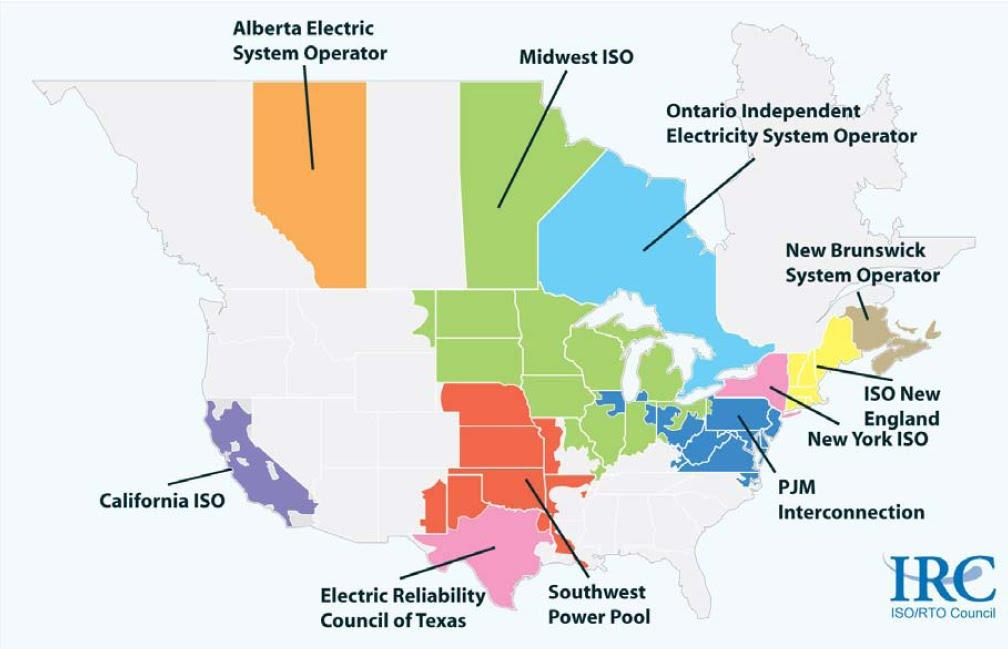
\includegraphics[scale=0.4]{anexos/mercados-eua.png}
\par\end{centering}

\caption{\label{fig:mercado-eua}A existência ou não de mercados de energia são definidos estado a estado nos EUA}
\end{figure}


Já as etapas de distribuição e transmissão são consideradas como monopólios
naturais. Entende-se por monopólio natural mercados que necessitam de
investimentos iniciais muito elevados e custos marginais muito baixos
e, com isso, a existência de concorrência poderia tornar impraticável
a existência de empresas que desejassem ofertar o serviço. Com isso,
é eficiente um esquema em que apenas uma empresa oferece o serviço
e este é regulamentada pelo governo. 

Faz parte do escopo deste trabalho, também, entender como oferecer os incentivos para que o mercado opere de forma eficiente. Se em um dado momento os atores não forem remunerados de forma adequado, gera-se um desincentivo para que novas empresas decidam entrar no negócio, diminuindo a competição e piorando a eficiência do mercado em médio prazo. 



%\subsection{Abertura do mercado no brasil}

\todo[inline]{incluir algo sobre a história da energia elétrica no brasil após a aula deste assunto}

O Brasil, assim como toda a América Latina, possui um alto percentual de usinas hidrelétricas em sua matriz energética. A figura \ref{fig:hidro-america-sul} mostra o percentual que essas usinas representam para cada país que possui mercado, assim como a existência ou não de um mercado de energia. 
Como mencionado anteriormente, a dependência de recursos hídricos (e de renováveis em geral) gera uma complexidade a mais para lidar quando planejamos o despacho das usinas. Para as usinas que possuem represa, é possível controlar seu estoque de água (até certo limite, claro) e decidir quando gerar energia com o que está no reservatório. No entanto, a quantidade de chuva em cada período é extremamente difícil de ser prevista. 
Podemos fazer decisões de consumo num período $t$ contando com chuva em $t+1$, mas se essa chuva não vir é possível que tenhamos que demandar uma alta quantia de energia de um tipo de usina mais custoso, como a termelétrica. Nesse e em outros casos, se faz necessária a mensuração do risco que corremos ao fazer decisões e não tomar decisões que possam colapsar o sistema com certa probabilidade. 


\begin{figure}[h]
\begin{centering}
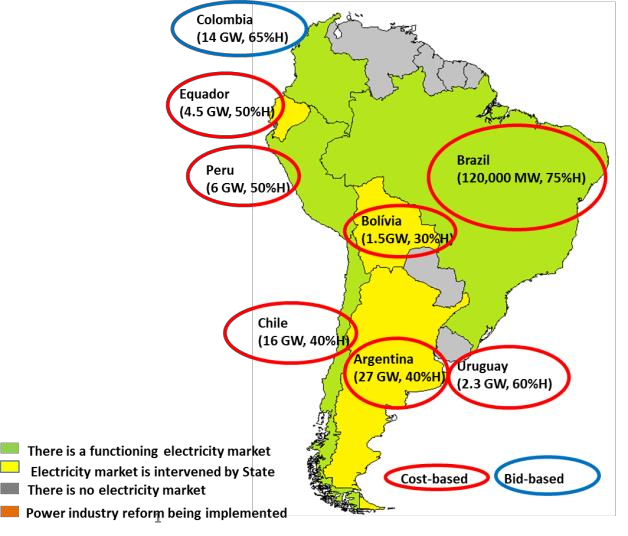
\includegraphics[scale=0.6]{anexos/hidro-america-sul.png}
\par\end{centering}

\caption{\label{fig:hidro-america-sul} Percentual de energia gerada por meio de usinas hidrelétricas e característica do mercado de energia por país}
\end{figure}


% Conclusão
Para realizar todas as atividades citadas acima, é preciso possuir
conhecimento de diversas áreas. A economia da energia elétrica é,
assim, um assunto multidisciplinar, que envolve disciplinas tão distintas
como economia, otimização, estatística, finanças e engenharia elétrica.
Uma visão global do processo de geração, assim como do funcionamento
do mercado de energia e sua interação com os consumidores, é exigida
do engenheiro elétrico do século XXI, não mais somente conhecimento
sobre capacitores e fluxos de potência. 



%%%%%%% OTIMIZAÇÃO %%%%%%%%%%%

\subsection{Revisão Otimização}
Esta sessão tem como objetivo apresentar os conceitos básicos de otimização que serão utilizados no decorrer do curso. Um modelo de otimização consiste em encontrar o valor máximo (mínimo) de uma \textbf{função objetivo}, por exemplo, o custo de geração de energia. Esta função possui um \textbf{vetor de variáveis de decisão} e é limitada por uma série de outras funções chamadas \textbf{restrições}.

Suponha que você é um dono de uma fábrica de móveis e deve decidir quais móveis produzir afim de obter o maior lucro possível. A fábrica produz armários e berços, que são representados pelas letras $A$ e $B$ respectivamente. No entanto, a quantidade produzida é limitada pelo estoque de matéria prima da fábrica, sendos estas madeira e ferro, representadas por $M$ e $F$. Sabemos que a receita líquida de um armário é de 4 reais e a do berço de 3 reais. Além disso, para se produzir um armário são necessárias 2 unidades de ferro e 1 unidade de madeira, e para o berço 1 unidade de ferro e 2 unidades de madeira. A fabrica possui 4 unidades de cada insumo em estoque. O problema pode se resumido em uma \textbf{matriz de tecnologia} apresentada na tabela \ref{tabela1}.

\begin{table}[H]
\begin{center}

\begin{tabular}{l|l|l|ll}
               & Armário & Berço & Estoque &  \\ \cline{1-4}
Ferro          & 2       & 1     & 4       &  \\ \cline{1-4}
Madeira        & 1       & 2     & 4       &  \\ \cline{1-4}
Lucro Marginal & 4       & 3     &         & 
\end{tabular}
\caption{Matriz de Tecnologia da Fábrica}
\label{tabela1}
\end{center}
\end{table}

Para encontrar o lucro ótimo devemos primeiro responder às seguintes perguntas:
\begin{itemize}
\item Quais são as variáveis de decisão do modelo?
\item Qual é a função objetivo do modelo?
\item Quais são as restrições do modelo?
\end{itemize}

A função objetivo é aquela que desejamos maximizar, no caso, o lucro. As variáveis de decisão são aquelas que devemos escolher afim de chegar ao resultado ótimo, ou seja, a quantidade produzida de cada móvel. As restrições do modelo são geradas pelas limitações do estoque. 

Formulação do problema:
\begin{itemize}
\item Variáveis de decisão: quantidade a produzir de cada produto $x_{A}$ e
$x_{B}$.
\item Função objetivo $f(x_{A},x_{B})=4x_{A}+3x_{B}$
\item Restrições:



\begin{itemize}
\item A quantidade de madeira utilizada não pode ser maior que o estoque:
$2x_{A}+1x_{B}\leq4$
\item A quantidade de ferro utilizada não pode ser maior que o estoque:
$1x_{A}+2x_{B}\leq4$
\item Não é permitido produzir quantidades negativas de armário ou berço: $x_{A}\geq0$ ,$x_{B}\geq0$\end{itemize}
\end{itemize}

Existe uma forma correta de escrever o problema acima com todas as suas informações. Em geral, é assim que você vai encontrar problemas de otimização e é assim que você deve procurar escreve-los. 

\begin{align}
    & \underset{x_A, x_B\geq0}{\text{maximizar}} \hspace{1cm} 4x_A+3x_B \label{eq1} \\
    & \text{s.a}  \hspace{2.2cm} 2x_A+x_B \leq 4; \label{eq2} \\
    &             \hspace{2.65cm} x_A+2x_B\leq 4, \label{eq3}
\end{align}

Em primeiro lugar temos a função objetivo, identificando se o problema é uma maximização ou uma minimização. É comum identificar o domínio das variáveis de decisão embaixo da palavra maximizar, neste caso, estamos dizendo que a quantidade produzida de cada móvel deve ser um número real não negativo. Entretanto, identificar o domínio e incluir as restrições $x_A, x_B \geq 0$ são exatamente a mesma coisa. 

Agora que já conhecemos o problema, temos que resolve-lo. Vamos colocar cada uma das restrições em um gráfico para entende-las melhor. 

\begin{figure}[H]
\begin{centering}
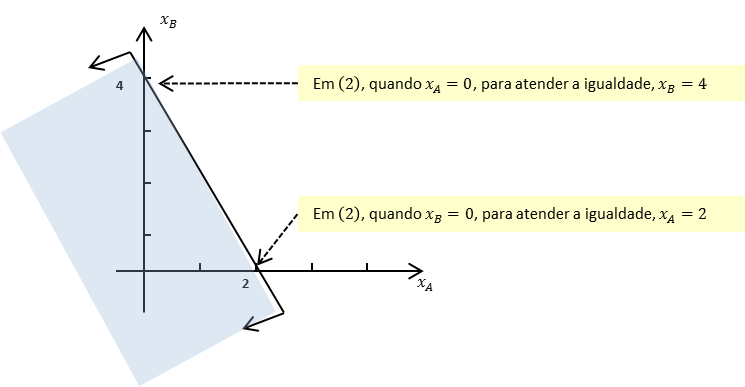
\includegraphics{pl1}\protect\caption{\label{fig:pl1}Gráfico equação (\ref{eq2})}
\end{centering}

\end{figure}

O que a figura \ref{fig:pl1} significa? No eixo $x$ temos a quantidade produzida de $x_A$ (armários), e no eixo $y$ a quantidade produzida de $x_B$ (berços). A reta desenhada na figura representa a restrição da equação \ref{eq2}. Todos os pontos a esquerda da reta são factíveis considerando apenas esta restrição. Como sabemos disso? Observe que pela restrição, se produzirmos apenas armários, a quantidade máxima produzida será 2 considerando as limitações de estoque, no caso dos berços, a quantidade será 4. Como a restrição é linear, e conheçemos dois pontos desta reta, basta ligar estes dois pontos para termos a representação gráfica da restrição.

De forma análoga, a figura \ref{fig:pl2} mostra a restrição escrita na equação \ref{eq3}.

\begin{figure}[H]
\begin{centering}
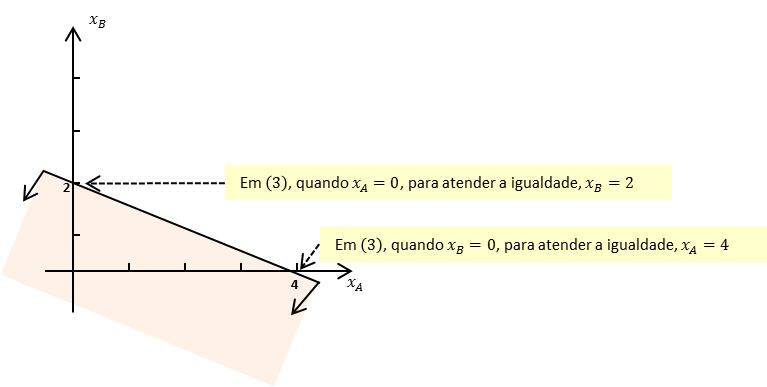
\includegraphics{pl2}\protect\caption{\label{fig:pl2}Gráfico equação (\ref{eq3})}
\end{centering}

\end{figure}

O conjunto de pontos viáveis pode ser encontrado combinando as duas figuras e levando em conta o domínio das variáveis de decisão. 

\begin{figure}[H]
\begin{centering}
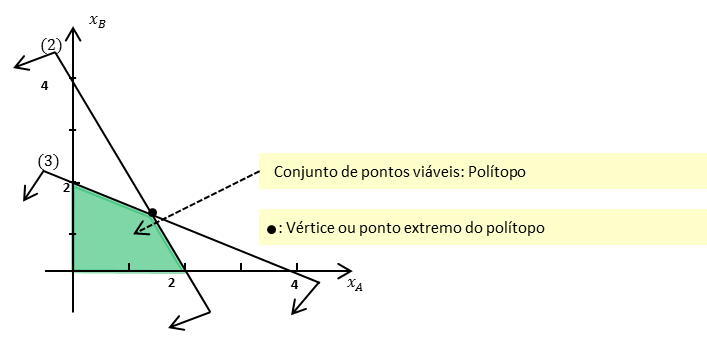
\includegraphics{pl3}\protect\caption{\label{fig:pl3}Gráfico conjunto de pontos viáveis}
\end{centering}

\end{figure}

Todos os pontos que estão na área verde da figura \ref{fig:pl3} são factíveis para a solução do nosso problema de otimização, porém apenas um deles é aquele que maximiza o lucro. Esta área é chamada de \textbf{poliedro}. Vamos encontrar qual o ponto ótimo utilizando o \textbf{gradiente}\footnote{Gradiente é o vetor das derivadas parciais da função objetivo.} da função objetivo para ver em qual direção que cresce mais rápido. Como se trata de uma função linear, o gradiente é constante e igual ao vetor $[4,3]$, representado na figura \ref{fig:pl4}.

\begin{figure}[H]
\begin{centering}
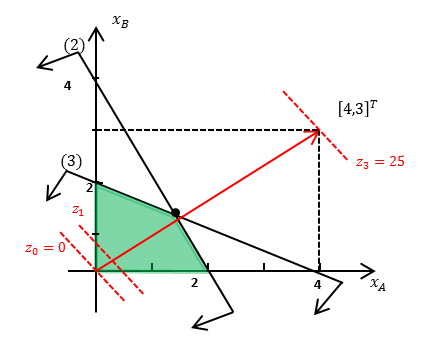
\includegraphics{pl4}\protect\caption{\label{fig:pl4}Gráfico curva de nível}
\end{centering}
\end{figure}

Com o gradiente podemos encontrar as \textbf{curvas de nível}, que são pontos onde a função objetivo tem o mesmo valor. As curvas de nível são perpendiculares ao vetor gradiente e também estão representadas na figura \ref{fig:pl4}. Finalmente, podemos resolver o problema caminhando com as curvas de nível para a direita até que ela chegue no último ponto dentro do poliedro dos pontos viáveis. 

\begin{figure}[H]
\begin{centering}
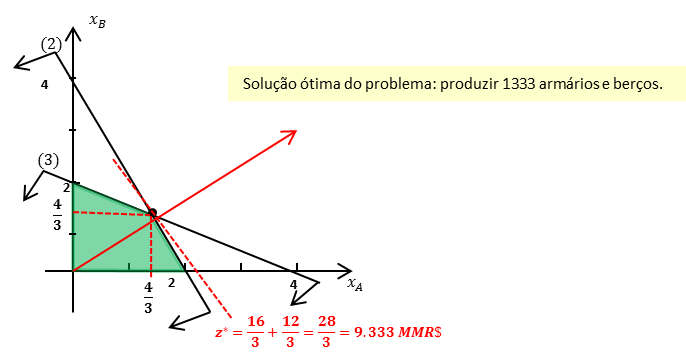
\includegraphics{pl5}\protect\caption{\label{fig:pl5}Gráfico solução ótima}
\end{centering}
\end{figure}

A figura \ref{fig:pl5} mostra a solução do problema. o Lúcro máximo é de $9.33$ reais e a solução ótima é aquela onde $x_A=x_B=\frac{4}{3}$.


Vamos colocar os passos para a resolução do problema de otimização acima em uma forma mais geral. Existem quatro passos básicos para se modelar um problema:
\begin{enumerate}
\item Compreensão do problema: 

\begin{itemize}
\item Identificar das partes relevantes o que se deseja tratar. Nesta parte,
geralmente são excluidas uma série de relações que não implicam em
uma direta, ou substancial, participação no objetivo do problema.
\end{itemize}
\item Identificação das variáveis de decisão: $x=[x_{1},...,x_{n}]^{T}$

\begin{itemize}
\item Quais são as variáveis que se deseja obter com a resolução do problema,
ou seja, o que se deseja encontrar (otimizar) e os seus respectivos
limites superiores e inferiores.
\end{itemize}
\item Identificar a função objetivo do problema: $f(x)$

\begin{itemize}
\item Especificar uma função que, dado uma possível configuração das variáveis
de decisão, reproduza o valor que se deseja maximixar ou minimixar
(otimizar): lucro, custo, confiabilidade, chance de se obter algum
resultado, distância de algum nível de referência,etc...
\end{itemize}
\item Identificar as condições que as variáveis devem atender: $g_{i}(x)\leq0$
para $i=1,...,m$

\begin{itemize}
\item Para serem válidas (viáveis) de serem escolhidas, através de inequação
ou equações.
\item É importante ressaltar que se uma possível solução não atender a alguma
das restrições, isso implica em descartar totalmente esta solução,
independentemente do valor da sua função objetivo. Logo, se existir
alguma possibilidade de discussão sobre o trade-off entre uma possível
violação e o valor da função objetivo, isso deve ser incoporado no
modelo.
\end{itemize}
\end{enumerate}

O problema do lucro ótimo da fábrica de móveis é uma \textbf{programação linear}, ou seja, tanto a função objetivo quanto as restrições são equações lineares. Todo problema de programação linear pode ser representado pela forma geral apresentada abaixo:

Forma compacta matricial
\begin{equation*}
\begin{aligned}
& \underset{x\geq0}{\text{maximizar}}
& & c^{T}x \\
& \text{s.a}
& & Ax \leq b.
\end{aligned}
\end{equation*}

Forma canônica,

\begin{equation*}
\begin{aligned}
& \underset{x}{\text{maximizar}}
& & \sum_{j=1}^{n}c_{j}\cdot x_{j} \\
& \text{s.a}
& &\sum_{j=1}^{n}a_{ij}\cdot x_{j}\leq b_{i},\qquad\forall i=1,...,m\\
& & & x_j \geq0\qquad\forall j=1,...,n.
\end{aligned}
\end{equation*}

Olhando para a forma matricial, $c$ são os coeficientes da função objetivo (4 e 3 no caso do exemplo da fábrida de móveis); $x$ são as variáveis de deicisão; $A$ é a matriz com os coeficientes das restrições; e $B$ representa o limite das restrições (no caso, o tamanho dos estoques). 
%\\

\textbf{\textit{Teoria da Dualidade}}

%\\

O \textbf{problema primal} é aquele problema que temos nas nossas mãos para resolver. Para obter algumas informações sobre o problema primal podemos utilizar o \textbf{problema dual}. No caso de uma máximização, o problema dual nos fornece um limite superior para o problema primal, se este limite superior for factível ele será o ótimo do problema primal. Isto pode ser reduzido em dois teoremas. 

\newtheorem{teo}{Teorema}[section]
\begin{teo}[Dualidade Forte]
Em um problema de programação linear, a solução ótima do problema primal será igual à solução ótima do problema dual se ambos forem viáveis. 
\end{teo}

\begin{teo}[Dualidade Fraca]
As soluções viáveis do problema dual são maiores ou iguais à solução do problema primal em um problema de maximização. No caso de um problema de minimização as relações são invertidas. 
\end{teo}


Voltando para o exemplo do problema de maximização do lucro da fábrica de móveis, lembre-se que ele era representado da seguinte forma:

\begin{align}
    & \underset{x\geq0}{\text{maximizar}} \hspace{1cm} 4x_A+3x_B \label{eq4} \\
    & \text{s.a}  \hspace{2.2cm} 2x_A+x_B \leq 4; \label{eq5} \\
    &             \hspace{2.65cm} x_A+2x_B\leq 4, \label{eq6}
\end{align}

Imagine que madeira e ferro estejam em falta no mercado, e que um comerciante deseja comprar o nosso estoque. Naturalmente, aceitaremos valores \todo{Revisar  valores de que}que, no total, sejam superiores ao nosso lucro fabricando os berços e armários. O problema do comerciante é minimizar o valor pago pelos nossos insumos levando em conta que nós só venderemos se o valor pago for maior do que o nosso lucro com a venda de berços e armários. As variáveis de decisão passam então a ser os preços dos insumos (madeira e ferro). O problema do comerciante é um problema dual do nosso problema de maximização do lucro. 

Vamos montar o problema do comerciante na forma de programação linear. A solução ótima do exemplo atende todas as restrições então, ao multiplicarmos a restrição \ref{eq4} por 3, obteremos a seguinte inequação, válida para todos os pontos viáveis.

\begin{equation}
6x_{A}+3x_{B}\leq12
\label{eq:dual1}
\end{equation}

Todos os coeficientes da desigualdade acima são maiores ou iguais do que seus respectivos coeficientes na função objetivo do problema de máximização de lucro, portanto o lucro será sempre menor do que 12.

Se fizermos uma combinação linear positiva das restrições (\ref{eq4}) e (\ref{eq5}), multiplicando-as pelo preço de cada insumo, representados por $y_A$ e $y_B$, a desigualdade será valida para todos os pontos que atendem às restrições originais:

\begin{table}[h]
\begin{center}
\begin{tabular}{lllll}
 & $y_{A}\cdot(2\cdot x_{A}+1\cdot x_{B})\leq y_{A}\cdot4$
 &  &  &  \\
 & $y_{B}\cdot(1\cdot x_{A}+2\cdot x_{B})\leq y_{B}\cdot4$ \hspace{1.0cm} + &  &  &  \\ \cline{2-2}
 & $(y_{A}\cdot2+y_{B}\cdot1)\cdot x_{A}+(y_{A}\cdot1+y_{B}\cdot2)\cdot x_{B}\leq y_{A}\cdot4+y_{B}\cdot4$ &  &  & 
 &   &  & % & 
\end{tabular}
\end{center}
\end{table}

Assumindo os valores $y_{A}=5/3$ e $y_{B}=2/3$, por exemplo, obteremos um
limite superior igual a $28/3$ , que sabemos ser o máximo do problema
da maximização do lucro. Isso nos mostra que o limite superior obtido por essa
escolha de multiplicadores resulta no menor limite possível, ou seja
, o limite ótimo. O teorema da dualidade forte garante que o GAP (diferença entre a solução dual e a primal) em problemas de otimização linear será sempre zero. Olhando para a figura \ref{fig:dualgap}

\begin{figure}[H]
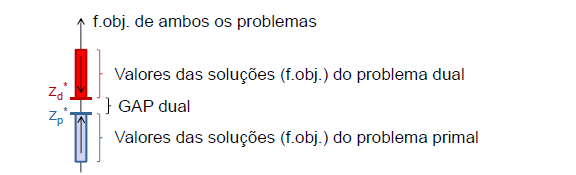
\includegraphics{pl6}\protect\caption{GAP dual}
\label{fig:dualgap}
\end{figure}


Retornando a resolução do problema em $y_{i},$ como podemos gerar
uma sistemática para encontrar os pesos de maneira que eles proporcionem
o menor limite superior (mínimo)?

Será necessário impor que cada coeficiente\footnote{Entenda como coeficiente toda a expressão que multiplica $x_A$ ou $x_B$.} da desigualdade encontrada
seja superior ao respectivo coeficiente da função objetivo : $z_{p}=4\cdot x_{A}+3x_{B}$

\begin{equation}
y_{A}\cdot2+y_{B}\cdot1\geq4
\end{equation}

\begin{equation}
y_{A}\cdot1+y_{B}\cdot2\geq3
\end{equation}

Com isso, o lado direito dessa nova desigualdade será sempre maior
que qualquer valor que a função objetivo possa valer dentro do conjunto
de pontos viáveis:

\begin{equation}
4\cdot x_{A}+3x_{B}\leq(y_{A}\cdot2+y_{B}\cdot1)\cdot x_{A}+(y_{A}\cdot1+y_{B}\cdot2)x_{B}\leq y_{A}\cdot4+y_{B}\cdot4
\end{equation}

Assim, queremos minimizar o limite superior, mexendo nos multiplicadores
$y_{i}$, sujeita a esses multiplicadores gerarem um limite superior:

\begin{align}
    & \underset{y\geq0}{\text{minimizar}} \hspace{1cm} 4y_A+4y_B \label{eq6} \\
    & \text{s.a}  \hspace{2.2cm} 2y_A+y_B \geq 4; \label{eq7} \\
    &             \hspace{2.65cm} y_A+2y_B\geq 3, \label{eq8}
\end{align}

O problema acima é um problema dual da programação linear da maximização do lucro. Ao mesmo tempo, ele é o problema do comerciante que deseja comprar nosso estoque. Ao solucionar o problema do comerciante (dual) encontramos os preços pelos quais seriamos indiferentes entre produzir móveis ou vender insumos. A figura \ref{pldual1} mostra a solução do problema dual de forma análoga à que fizemos para o problema primal. 

\begin{figure}[H]
\begin{centering}
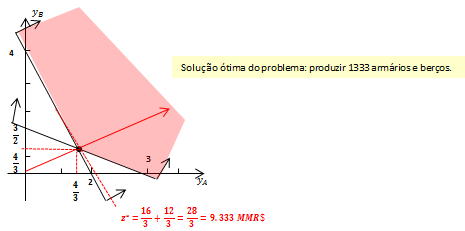
\includegraphics{pldual1}\protect\caption{\label{pldual1}Solução do problema dual}
\end{centering}
\end{figure}


De forma geral, um problema de programação linear definido como: 

\begin{equation*}
\begin{aligned}
& \underset{x\geq0}{\text{maximizar}}
& & c^{T}x \\
& \text{s.a}
& & Ax \leq b.
\end{aligned}
\end{equation*}

Tem a seguinte representação dual:

\begin{equation*}
\begin{aligned}
& \underset{y\geq0}{\text{minimizar}}
& & y^{T}b \\
& \text{s.a}
& & Ay^{T} \geq c.
\end{aligned}
\end{equation*}


\subsection{Revisão Estatística}

Otimização e estatística caminham juntas, principalmente quando estamos resolvendo problemas mais complexos. Imagine que queremos modelar um contrato de um parque eólico no ambiente livre (ACL). Para determinar o contrato, precisamos de projeções futuras da velocidade do vento, da potência gerada pelo parque e do preço da energia. Em outras palavras, precisamos gerar vários cenários possíveis para o futuro, e fazemos isto utilizando conceitos de estatística e de probabilidade. 

Como não sabemos o que vai acontecer no futuro, nossos cenários de possíveis realizações resultam em \textbf{distribuições de probabilidade}, e precisamos conhecer bem as características destas distribuições para construir cenários coerentes com a realidade. Uma distribuição de probabilidade descreve as chances de uma determinada variável assumir diferentes valores. Em outras palavras, uma distribuição é uma função que transforma valores de uma variável em probabilidade. 

Suponha que estamos jogando uma moeda. Os resultados possíveis são cara e coroa, se representarmos cara pelo número 1, e coroa por 0, temos o domínio de uma distribuição de probabilidade. A distribuição da moeda nos dirá que em $50\%$ das vezes o resultado será cara, e em $50\%$ será coroa. Esta distribuição é conhecida como \textit{distribuição de Bernoulli}.

A distribuição de Bernoulli é uma \textbf{distribuição discreta}. Em muitos casos pode ser interessante representar uma variável por uma \textbf{distribuição contínua}, ou seja, uma variável que pode assumir qualquer valor em um intervalo. A mais importante das distribuições contínuas é a \textbf{distribuição normal}. 
\\

\textbf{\textit{Distribuições Discretas}}


Já vimos que uma moeda pode ser caracterizada como uma distribuição discreta. Suponha agora que estamos jogando um dado. Ele pode assumir valores de 1 a 6 em intervalos discretos, ou seja, apenas os números inteiros de 1 a 6. A figura \ref{fig:prob1} apresenta o \textbf{histograma} de um dado. 

\begin{figure}[H]
\begin{centering}
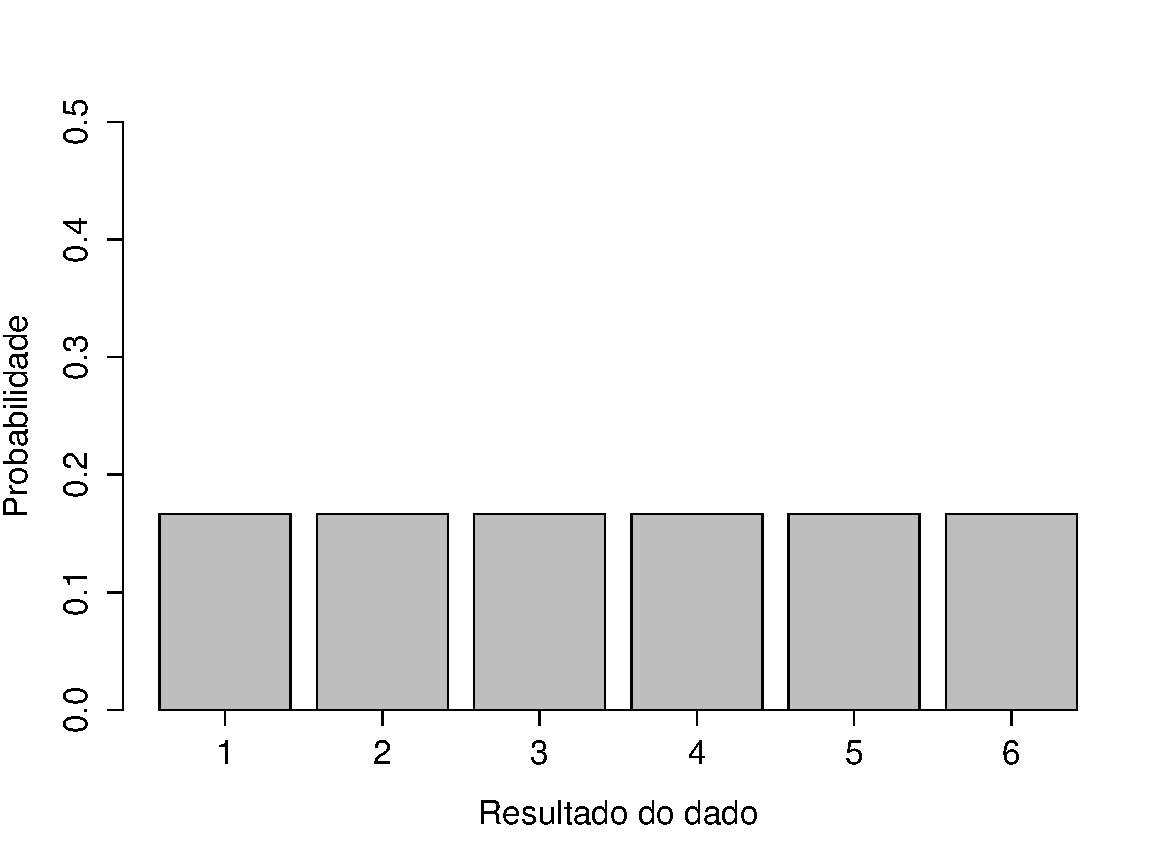
\includegraphics[scale=0.5]{uniforme-discreta}\protect\caption{\label{fig:prob1}Histograma de um dado}
\end{centering}
\end{figure}

No eixo $x$ temos os possíveis resultados do dado, ou seja, inteiros de 1 até 6. No eixo $y$ temos a probabilidade de cada resultado igual a $\frac{1}{6}$. Esta é uma \textbf{distribuição uniforme discreta}. O histograma apresenta os valores da variável no eixo $x$ e a probabilidade no eixo $y$. Entretanto, pode ser interessante olhar para a distribuição de probabilidade em sua forma acumulada, e não na forma de densidade como no histograma. 

\begin{figure}[H]
\begin{centering}
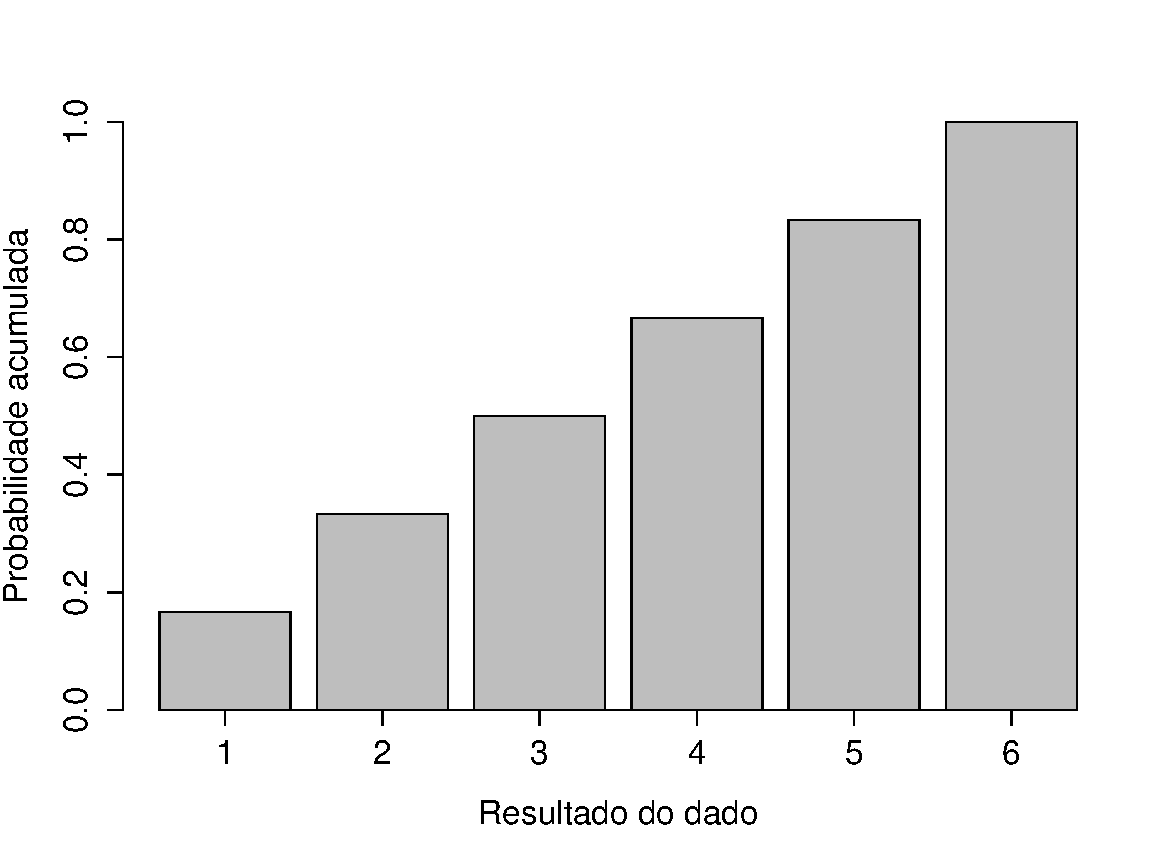
\includegraphics[scale=0.5]{uniforme-discreta-acumulada}\protect\caption{\label{fig:prob2}Distribuição acumulada de um dado}
\end{centering}
\end{figure}

A figura \ref{fig:prob2} mostra a mesma distribuição da figura \ref{fig:prob1}, porém em sua forma acumulada. No caso, a função acumulada em 4, por exemplo, representa a probabilidade de tirarmos um número menor ou igual a 4 no dado, $p(x\leq4)$. Observe que a distribuição acumulada termina onde a probabilidade assume o valor 1, ou $100\%$. Isto é o mesmo que dizer que com $100\%$ de chance tiraremos um número menor ou igual a 6 no dado, o que é verdade. No caso discreto, a distribuição acumulada terá sempre esta forma de escada, e o histograma poderá ser representado na forma de barras (fig. \ref{fig:prob1}).


Podemos escrever a distribuição do dado como uma fórmula matemática, no caso da densidade:

\begin{equation}
f(x)=p(x)=\frac{1}{6},~~~x\in [1,2,3,4,5,6]
\end{equation}

No caso da função acumulada:

\begin{equation}
F(x)=p(X\leq x)=\frac{1}{6}x,~~~x\in [1,2,3,4,5,6]
\end{equation}

Por convensão, usamos $f$ minúsculo para a função densidade e $F$ maiúsculo para a função acumulada. Além disso, o $X$ maiúsculo representa a variável aleatória do dado, e o $x$ minúsculo representa uma realização da mesma. Podemos escrever $p(X\leq 3)=\frac{1}{2}$, por exemplo. 

Por último, é interessante calcular a média e a variância das distribuições de probabilidade. A média é uma medida de \textbf{tendência central} e a variância mede a \textbf{dispersão} em torno da média. 

\begin{itemize}
\item média $=E[X]=\sum_{i=1}^n p_i x_i$
\item variância $=\sigma^2(X)=\sum_{i=1}^n p_i (x_i-E[X])^2$
\end{itemize}

onde, $p_i$ é a probabilidade do resultado $i$ acontecer. No caso da distribuição do dado esta probabilidade é igual a $\frac{1}{6}$ para todo $i$.

No caso do dado, a média e a variância são iguais a $3.5$ e $2.9$ respectivamente. Entretanto, a variância é uma medida difícil de interpretar. Imagine que estamos diante de uma distribuição de potência, a variância será medida então em potência ao quadrado. Para voltarmos para potência basta calcular o \textbf{desvio padrão}, que é a raiz quadrada da variância.\\



\textbf{\textit{Distribuições Continuas}}

Uma distribuição é contínua se seu domínio for contínuo. A mais conhecida das distribuições contínuas é a distribuição normal, seu histograma é apresentado na figura \ref{fig:prob3} e sua distribuição acumulada na figura \ref{fig:prob4}. 


\begin{figure}[H]
\begin{centering}
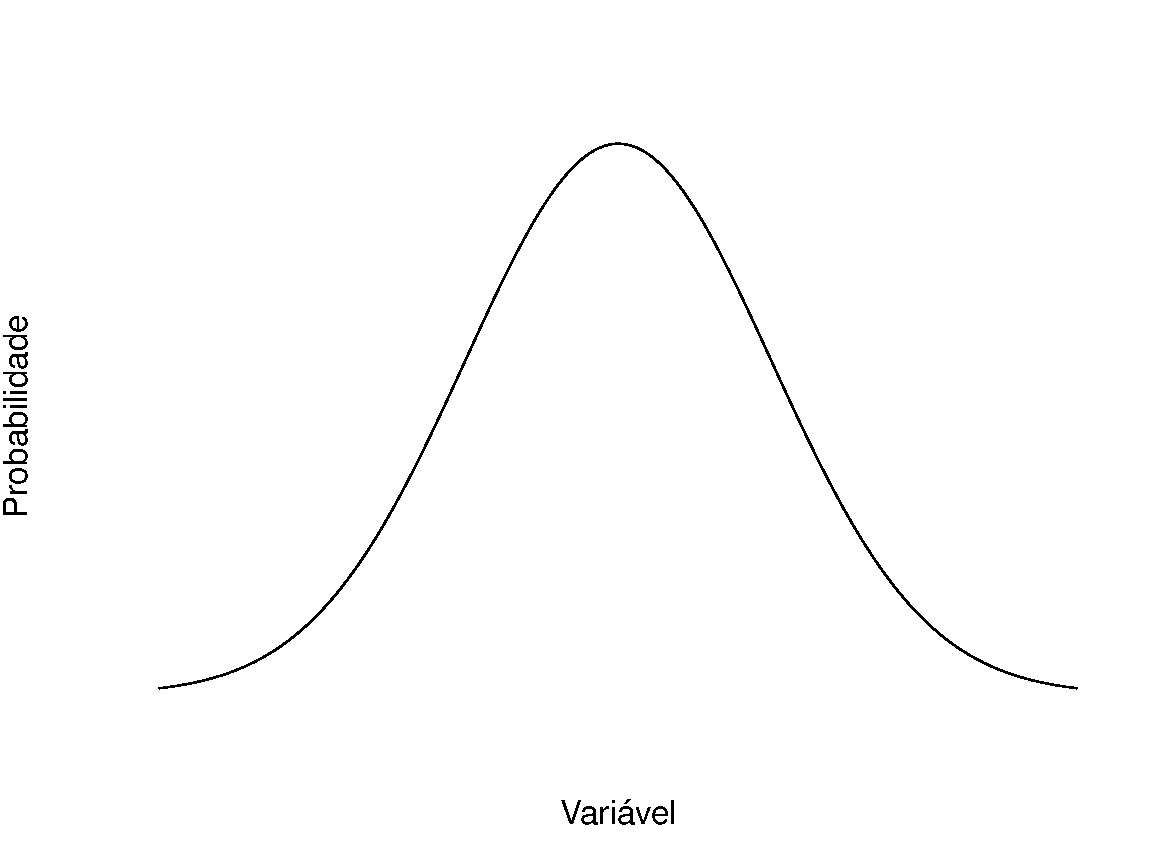
\includegraphics[scale=0.5]{histograma-normal}\protect\caption{\label{fig:prob3}Distribuição normal}
\end{centering}
\end{figure}

\begin{figure}[H]
\begin{centering}
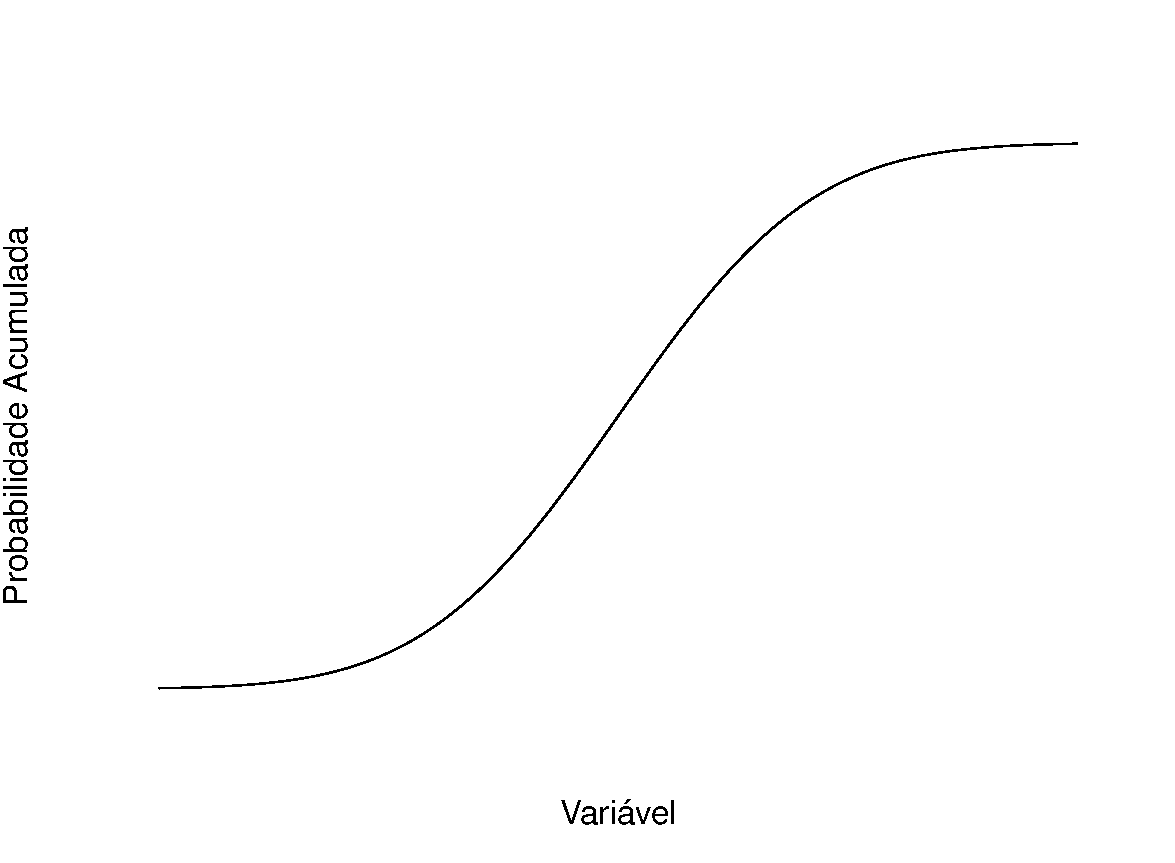
\includegraphics[scale=0.5]{histograma-normal-acumulada}\protect\caption{\label{fig:prob4}Distribuição normal acumulada}
\end{centering}
\end{figure}

O histograma de uma distribuição contínua não pode mais ser desenhado na forma de barras, e a distribuição acumulada não terá mais a forma de escada. Entretanto, a interpretação é muito semelhante à do caso discreto. Como uma distribuição contínua tem infinitos pontos no domínio, falar da probabilidade de ocorrência de um ponto isolado perde o sentido, pois esta probabilidade será igual a zero. O mais usual é falar da probabilidade de intervalos, por exemplo, a probabilidade de $x$ estar entre 1 e 2. 

Assim como no caso discreto, podemos representar as distribuições contínuas com uma fórmula, no caso da normal:

\begin{equation}
f(x)=\frac{1}{\sqrt{2 \pi \sigma^2}} e^{-\frac{(x-\mu)^2}{2\sigma^2}}
\end{equation}

A fórmula da distribuição acumulada da normal não é conhecida, entretanto, ela já foi toda tabelada e podemos utiliza-la sem problemas. Observe que na fórmula da normal temos os parâmetros $\mu$ e $\sigma^2$, que são respectivamente a média e a variância da distribuição. Portanto, se uma certa variável é normal e conhecemos sua média e sua variância, conhecemos também toda a distribuição desta variável.

Para calcular a média e a variância de uma distribuição contínua temos que calcular uma soma de infinitos elementos, por isto, o somatório é substituido pela integral.

\begin{itemize}
\item média $=\mu_X =E[X]=\int_{-\infty}^{\infty} xf(x)dx$
\item variância $=\sigma^2_X=\int_{-\infty}^{\infty} (x-E[X])^2 f(x)dx$  \end{itemize}
%\\

\textbf{\textit{Quantis}}

Uma fórma interessante de olhar para uma distribuição é separando-a em \textbf{quantis}. Quantis são pontos no domínio da distribuição acumulada que separam a mesma em intervalos iguais. Por exemplo, suponha que dividimos uma distribuição em quatro quantis\footnote{A divisão em quatro quantis é conhecida como quartil.}, a probabilidade de um elemento do domínio estar em um destes quantis é de $25\%$, e um mesmo elemento nunca estará em dois quantis ao mesmo tempo. 

Para ilustrar, suponha uma distribuição que assume os valores inteiros $[1,1,4,6,7,11,12,12]$. O primeiro quantil será $[1,1]$; o segundo será $[4,6]$, o terceiro será $[7,11]$ e o quarto será $[12,12]$. O segundo quartil, também chamado de mediana, divide a amostra no meio. A mediana é uma medida de tendência central assim como a média.

Quantis são muito úteis quando queremos estudar partes separadas das distribuições. Imagine uma distribuição de geração de um parque eólico, se queremos ver quais são os $5\%$ piores cenários de geração do nosso parque, basta separar a distribuição em 100 quantis e pegar os primeiros 5.

%\section{Aula 2}

\subsection{História da Energia Elétrica}


\subsubsection{Evolução da energia elétrica}

Este capítulo contará um pouco sobre a história da energia elétrica e como chegamos aonde estamos, partindo da invenção da lâmpada para complexos sistemas elétricos. A tablela \ref{linha-tempo} mostra um pouco desta história.

A primeira invenção que teve utilidade direta para as pessoas comuns foi feita em 1752 por Benjamin Franklin. O para raios foi o primeiro passo para o domínio da energia elétrica pelo homem. A partir daí as descobertas vieram cada vez mais rápido, e avanços teóricos permitiram o conhecimento das leis fundamentais da energia elétrica, como a lei de Ohm, que cria a relação entre corrente, tensão e resistência elétrica.

Estas descobertas culminaram na invenção da lçampada por Thomas Edison e posteriormente levaram ao conhecimento do elétron, que foi descoberto por J. J. Thomson. No entanto, ainda existiam grandes obstáculos para a popularização da energia elétrica. Os primeiros sistemas eram locais, e não havia qualquer tipo de conexão entre eles. Um fato curioso é que as pessoas não pagavam pelo consumo de energia, e sim pelas lâmpadas. 


\begin{table}[H]
\caption{\label{linha-tempo}Linha do tempo da energia elétrica}
\centering
\begin{minipage}[H]{.8\linewidth}
\color{gray}
\rule{\linewidth}{0.9pt}
\ytl{Pré-1700}{Até o século XVIII, estudos empíricos indicavam a existência de elementos
associados a eletricidade em experiências feitas com animais e elementos químicos} 
\ytl{1733}{Du Fay (Francês) publica a existência de dois tipos de eletricidade, o que
mais tarde seria identificado como "positivo" e "negativo". Ele também identifica a
diferença entre isolantes e condutores} 
\ytl{1752}{Benjamim Franklin, a partir de suas observações sobre descargas
atmosféricas, Franklin inventa o pára-raios}
\ytl{1800}{O conde Alessandro Volta desenvolve a pilha voltaica, precursora das
baterias modernas. A pilha de Volta era capaz de produzir corrente continua}
\ytl{1826}{André-Marie Ampere mostra que uma corrente elétrica apresenta uma
expressão que relaciona a corrente elétrica com a produção de um campo magnético}
\ytl{1827}{A lei de Ohm relaciona as grandezas fundamentais da
eletricidade: tensão, corrente e resistência elétrica}
\ytl{1832}{Faraday mostra como a variação do campo magnético pode gerar uma
corrente elétrica. 
Paralelamente, Gauss estabelece a relação entre carga elétrica dentro de uma
superfície de volume limitado e o campo elétrico que passa através de uma
superfície}
\ytl{1850}{James Clerk Maxwell encerra um ciclo da história da eletricidade ao formular as
equações que unificam a descrição dos comportamentos elétrico e magnético da
matéria. Esta é a teoria que surge juntando a lei de Ampere, a lei de Gauss e a lei de
Faraday}
\ytl{1873}{O cientista belga Zénobe Gramme demonstrou que a eletricidade
podia ser transmitida de um ponto a outro através de cabos condutores aéreos}
\ytl{1879}{Thomas Edison inventa a lâmpada incandescente. Dois anos depois
constrói na cidade de Nova York a primeira central de energia elétrica com
sistema de distribuição. Nesta época, o serviço de energia elétrica era vendido por lâmpadas, não
eletricidade}
\ytl{1890}{O descobrimento do elétron por Joseph John Thomson, na década de 1890 pode ser
considerado o marco da passagem da ciência da eletricidade para a da eletrônica, que
proporcionou um avanço tecnológico ainda mais acelerado}
\bigskip
\rule{\linewidth}{1pt}%
\end{minipage}%
\end{table}

\subsubsection{Guerra das correntes}

Um dos primeiros grandes debates na história da energia elétrica foi aquele conhecido como a Guerra das Correntes. De um lado estava Thomas
Edison ,com o financiamento do J.P Morgan, que propunha utilizar um
sistema de \textbf{corrente continua} para atender localmente as cidades; do outro lado estava Nicolas
Tesla, com o patrocínio de George Westinghouse, que propôs que
os sistemas elétricos deveriam se expandir a partir do que eles chamavam
de \textbf{corrente alternada}. 

Vamos entender o que são essas correntes. A corrente contínua é aquela onde existe um fluxo ordenado de elétrons sempre na mesma direção. Nos dias de hoje, este tipo de corrente é utilizado em baterias na maioria dos aparelhos eletrônicos portáteis que carregamos, como tablets, celulares, etc. Sempre que você ver algum aparelho elétrico com polo positivo e polo negativo, você estará lidando com corrente contínua. A corrente alternada, por outro lado, é aquela onde o sentido dos elétrons varia no tempo, em geral, na forma \textbf{senoidal}, ou seja, como ondas. A corrente que sai da nossa casa no Brasil é alternada, é por isso que nossos aparelhos eletrônicos possuem uma fonte. 

A ideia da corrente alternada seria diminuir as perdas elétricas com um aumento da tensão e uma redução da corrente. Edison argumentava que este tipo de aumento poderia ser perigoso.


% Figura corrente alternada
\begin{figure}[H]
\begin{center}
\fbox {
    \begin{tikzpicture}[domain=0:4]
        \draw[very thin,color=gray] (-0.1,-2.1) grid (3.9,2.1);
        \draw[->] (-0.2,0) -- (4.2,0) node[right] {$t$};
        \draw[->] (0,-2.2) -- (0,2.2) node[above] {$V$};
        \draw[smooth, color=blue] plot[id=sin] function{sin(5*x)} 
            node[right] {Corrente alternada};
    \end{tikzpicture}1
    }
\caption{\label{fig:corrente-alternada} Característica da corrente alternada}
\end{center}
\end{figure}




% Figura corrente contínua
\begin{figure}[H]
\begin{center}
\fbox {
    \begin{tikzpicture}[domain=0:4]
        \draw[very thin,color=gray] (-0.1,-0.1) grid (3.9,3.9);
        \draw[->] (-0.2,0) -- (4.2,0) node[right] {$i$};
        \draw[->] (0,-0.2) -- (0,4.2) node[above] {$V$};
        \draw[smooth, color=blue] plot[id=sin] function{2} 
            node[right] {Corrente contínua};
    \end{tikzpicture}
    }
\caption{\label{fig:corrente-continua}Característica da corrente contínua}
\end{center}
\end{figure}


Quem venceu a Guerra das Correntes foi a corrente alternada, no entanto, se a guerra fosse hoje, Edison teria mais argumentos, pois naquela época o único aparelho elétrico alimentado pelas correntes eram as lâmpadas.
.Hoje, como mencionado anteriormente, alguns equipamentos utilizam corrente contínua por exemplo:
celular, MP3 player e computador.

A guerra parece não ter terminado, além dos aparelhos que utilizam corrente contínua, estão surgindo formas de geração de energia, como painéis solares, que geram neste tipo de corrente. Painéis solares estão cada vez mais modernos e baratos, e em alguns países as pessoas já estão começado a utiliza-los em casa. Acredite se quiser, já existe até um mercado de aluguel de telhados, onde empresas pagam para colocar painéis em cima da sua casa. Apesar do mercado de energia solar brasileiro ainda ser muito pequeno, já existem geradores privados, como shopping centers que possuem muito espaço para colocar os painéis. 

As linhas de corrente contínua tem custo inicial muito alto, mas conforme a linha cresce este custo começa a ser diluído, pois uma vez instalada, aumenta-la é barato. As linhas de corrente contínua, por outro lado, possuem um custo inicial barato dado que as grande maioria dos geradores já geram em corrente contínua. Entretanto, aumentar a linha vai ficando cada vez mais caro. Em um país com as dimensões do Brasil vale a pena considerar a construção de linhas de corrente contínua, inclusive, uma linha está sendo construída ligando a região norte á região sudeste. 

\begin{figure}[H]
\begin{centering}
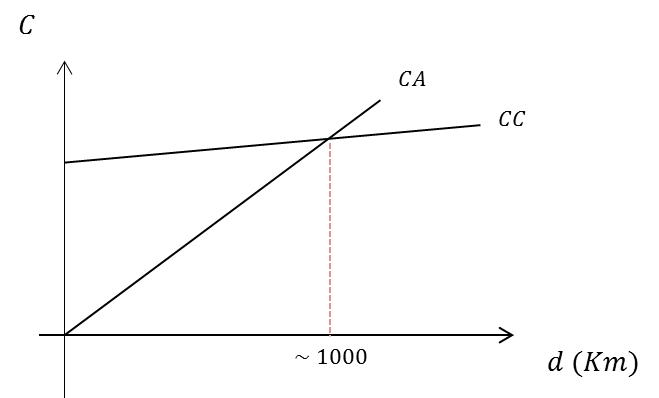
\includegraphics{aula2_3}\protect\caption{\label{fig:aula2_3} Corrente contínua e Corrente alternada }
\end{centering}

\end{figure}

\subsubsection{Sistemas elétricos em corrente alternada}

No sécilo XIX, o cientista ingês M. Faraday realizou o seguinte experimento: ele pegou uma pilha ,adicionou um chave para ligar e desligar essa pilha e colocou uma bobina com fios enrolados, fechando um circuito; do outro lado Faraday colocou um aparelho conhecido com galvanômetro, que tem a capacidade de detectar correntes elétricas, em um circuito fechado sem ligação com aquele da pilha. Então, a chave que estava aberta foi fechada, e o galvanômetro captou uma corrente mesmo estando em outro circuito. Faraday percebeu que o que levava à reação do galvanômetro era o fluxo magnético que conectava com o outro lado do experimento gerava uma corrente. Um ponto relevante no experimento é que Faraday sabia que a corrente provocava fluxo mas não sabia que fluxo provocava corrente. Então esse equipamento movia quando a chave era virada porem depois o equipamento voltava a posição inicial. Quando era desligada a chave, as linhas de fluxos desapareciam e o outro equipamento movia para o outro lado. Assim, quando era ligado o equipamento movimentava-se para um lado e quando desligado o movimento era contrário, invertendo assim o sentido (Figura \ref{fig:aula2_4}). 
\begin{figure}[H]
\begin{centering}
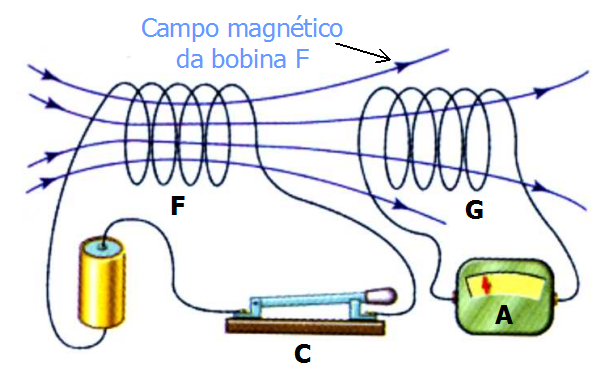
\includegraphics{aula2_4}\protect\caption{\label{fig:aula2_4}Experimento de M.Faraday }
\end{centering}

\end{figure}
Quem explicou e formalizou o experimento de Faraday foi Lenz, que descobriu a lei que levou o seu nome. A lei de Lenz postula que o sentido da corrente é o oposto da variação do campo magnético que lhe deu origem. O
experimento de Lenz é semelhante ao de Faraday, no entanto ele utilizou um imã para produzir as correntes de produzir linhas de fluxos provocados por correntes. Lenz injetou um campo magnético na espira, ou seja aproximou
o imã da espira e observou que quando aproxima o imã da espira
apareciam linhas de campo de sentido contrário ao movimento que foi
imposto. A medida que ele aproximava mais o imã apareciam linhas de campo no
sentido contrário, que induziam a passagem de corrente
elétrica nessa espira para recuperar o equilíbrio \ref{fig:aula2_5}. Assim,
Lenz (1834) respondeu porque a corrente elétrica mudava de sentido
quando se retirava o campo magnético.
\begin{figure}[H]
\begin{centering}
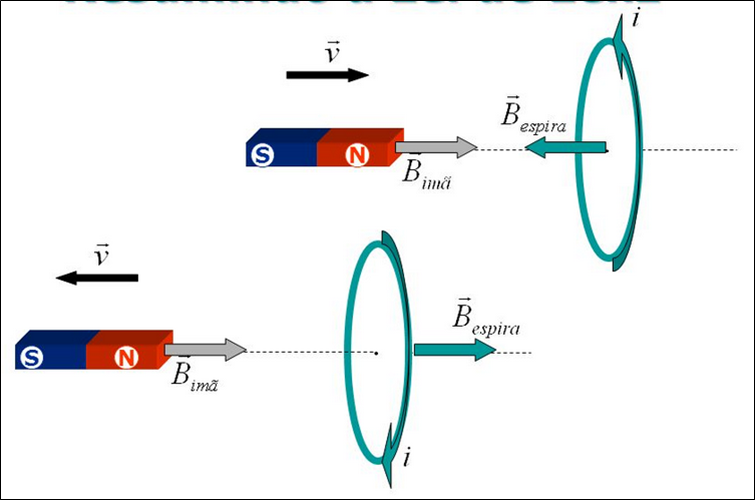
\includegraphics{aula2_5}\protect\caption{\label{fig:aula2_5}Experimento de Lenz }
\end{centering}

\end{figure}

A grandeza escalar que mede o número de linhas de indução que atravessam
a área \textit{\textcolor{black}{A }}de uma espira imersa num campo
magnético uniforme \ref{fig:aula2_6} é chamada fluxo magnético $(\Phi)$, sendo definida
por:
\begin{equation}\label{eq:fluxomag}
\Phi=n\cdot B\cdot A\cdot\cos\theta 
\end{equation}


onde,

$A$- área em $m^{2}$

$B$- campo magnético em tesla $(T)$

$\Phi$- fluxo magnético em weber $(Wb)$

$n$- número de espiras.




\begin{figure}[H]
\begin{centering}
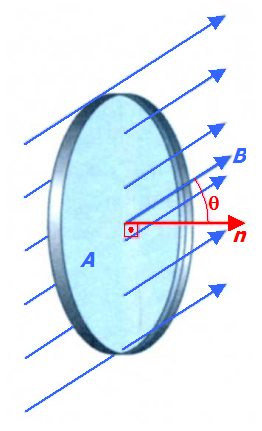
\includegraphics{aula2_6}\protect\caption{\label{fig:aula2_6}Fluxo magnético }
\end{centering}

\end{figure}
Assim, o fluxo magnético será proporcional ao número de espiras, a
intensidade das linhas de campos, a área da seção e oo cosseno de $\Theta$
(o angulo entre as linhas de campo magnético e a linha perpendicular
a espira). 
Por exemplo quando $\Theta=0$,fluxo máximo,$\cos\Theta=1$, então
$\Phi=n\cdot B\cdot A$ (Figura \ref{fig:aula2_7}); e quando $\Theta=90^{\circ}$,sem fluxos,$\cos\Theta=0$,
então $\Phi=0$ (Figura \ref{fig:aula2_8}).

\begin{figure}[H]
\begin{centering}
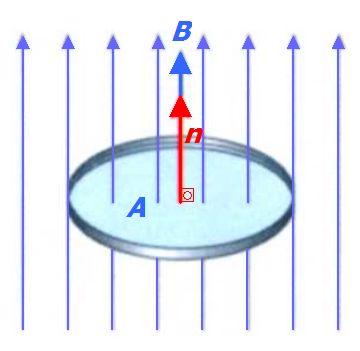
\includegraphics{aula2_7}\protect\caption{\label{fig:aula2_7}Fluxo máximo }
\end{centering}

\end{figure}
\begin{figure}[H]
\begin{centering}
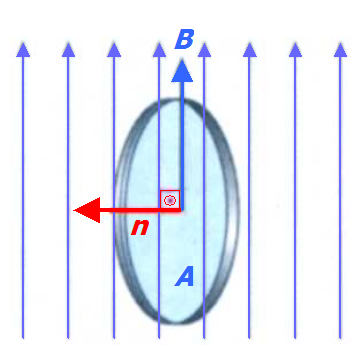
\includegraphics{aula2_8}\protect\caption{\label{fig:aula2_8}Sem fluxo }
\end{centering}

\end{figure}

O outro experimento é ao contrário, deixando o imã fixo e fazer girar
a espira, a experiência é semelhante ,mas trocou a função dos elementos.
Então a geração de energia elétrica será a partir de energia mecânica (Figura
\ref{fig:aula2_9}) . Assim, hora a tensão elétrica é produzida em um sentido, hora
em outro sentido caracterizando a corrente alternada.

\begin{figure}[H]
\begin{centering}
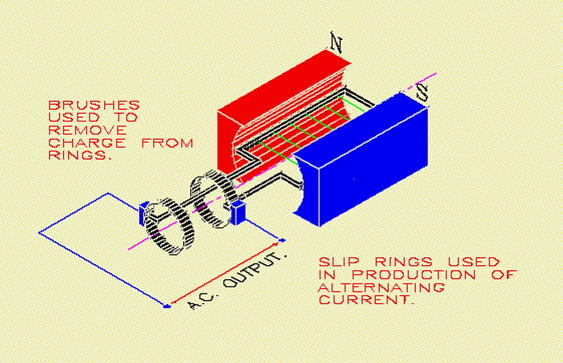
\includegraphics{aula2_9}\protect\caption{\label{fig:aula2_9}Experimento imã fixo }
\end{centering}

\end{figure}

Periodicamente, a variação de fluxo magnético na bobina (girando),
implica em uma tensão variável ao longo do tempo porque em cada hora
a bobina terá uma posição diferente (Figura \ref{fig:aula2_10}). Pela lei de Lenz a hora que injetamos
a variação de fluxo no tempo ela produz uma tensão que é contraria
ao movimento que gerou a tensão; e a posição da bobina em relação ao
campo magnético depende do tempo. Assim:

\begin{equation}\label{eq:et}
e(t)=\frac{\partial\Phi(t)}{\partial t}
\end{equation}

\begin{figure}[H]
\begin{centering}
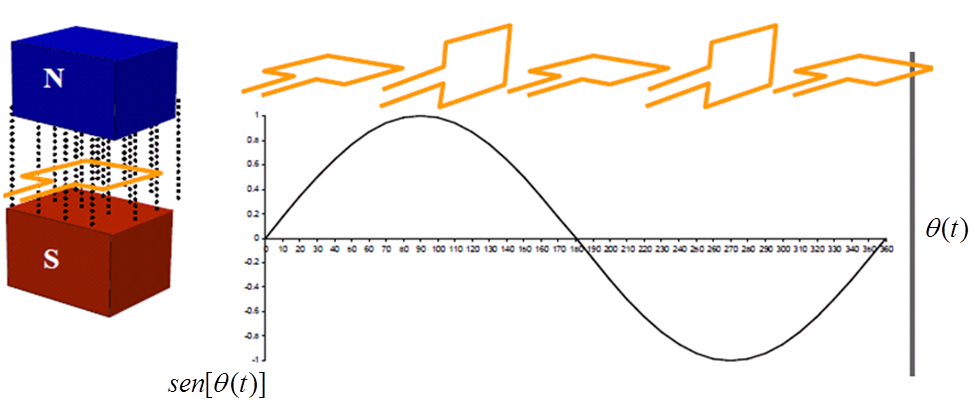
\includegraphics{aula2_10}\protect\caption{\label{fig:aula2_10}A posição da bobina }
\end{centering}

\end{figure}
Definindo $\omega$ como a velocidade angular da bobina. Pode-se escrever:

\begin{equation}\label{eq:omega}
\omega=\frac{\triangle\theta}{\triangle t}(\frac{rad}{seg})
\end{equation}

De outra forma:
\begin{equation}\label{eq:omega2}
\omega=\frac{\theta_{F}-\theta_{I}}{t_{F}-t_{I}}(\frac{rad}{seg})
\end{equation}

Considerando:

$\theta_{I}=0$ e $t_{I}=0$ então:
\begin{equation}\label{eq:omega3}
\omega=\frac{\theta_{F}}{t_{F}}=\frac{\theta}{t}
\end{equation}

Finalmente
\begin{equation}\label{eq:omega4}
\theta=\omega t
\end{equation}
A força eletromotriz $(e)$ em volts pode ser calculada como:

\begin{equation}\label{eq:ele}
e(t)=-\frac{\triangle\Phi(t)}{\triangle t}=-\frac{\partial[nBA\cos(\omega t)]}{\partial t}
\end{equation}

Assim,

$\Phi(t)=nBA\cos(\omega t)$

$e(t)=n\omega BA\sin(\omega t)$

$e(t)=E_{max}\sin(\omega t)$

$E_{max}=n\omega BA$

\begin{figure}[H]
\begin{centering}
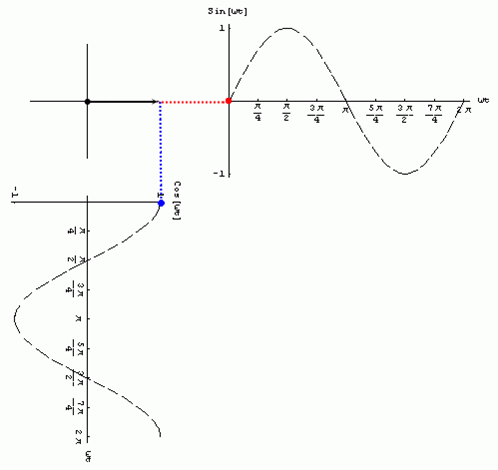
\includegraphics{aula2_11}\protect\caption{\label{fig:aula2_11}A posição da bobina }
\end{centering}

\end{figure}

Na Figura \ref{fig:aula2_11} a tensão e o fluxo variam no tempo.
Definindo $f$ como \textbf{frequência da rotação}. A frequência de rotação
descreve o numero de revoluções (voltas completas) por segundo da
bobina. Assim,

\begin{equation}\label{eq:freq}
f=\frac{n\text{º revoluções (voltas completas)}}{tempo(seg)}
\end{equation}

A unidade de frequência é hertz. Diz-se que o sistema tem um hertz
se a bobina efetua uma volta completa a cada segundo. No Brasil o
consumo em geral possui um frequência estabelecida de $60$ hertz
ou 377 radianos por segundo. 
A velocidade angular da bobina e, consequentemente, da tensão é ($2\pi$
é uma volta completa):

\begin{equation}\label{eq:omega6}
\omega=\frac{\triangle\theta}{\triangle t}(\frac{rad}{seg})
\end{equation}

De outra forma:
\begin{equation}\label{eq:omega7}
\omega=n\text{º revol.}(\frac{2\pi}{\triangle t})(\frac{rad}{seg})
\end{equation}

Então:
\begin{equation}\label{eq:omega8}
\omega=2\pi f
\end{equation}
Temos que:
\begin{equation}\label{eq:omega9}
\Phi=nBA\cos(2\pi ft)
\end{equation}

\begin{equation}\label{eq:omega10}
\ e(t)=(2\pi f)n\omega BA\sin(2\pi ft)
\end{equation}

\begin{equation}\label{eq:omega11}
[e(t)=E_{max}\sin(2\pi ft)]
\end{equation}
Trabalhar com grandezas no tempo é inconveniente no ponto de vista
matemático, então é comum mudar a forma de trabalhar com as grandezas
no setor elétrico. Como o sistema elétrico brasileiro está girando a 60 hertz,
então é tirada uma fotografia de um determinado ponto do sistema e
estabelecida
uma referencia, e ao invés de dizer que estão no domínio do tempo diz-se
que está no domínio da frequência . 
Para evitar a manipulação matemática das grandezas que variam no tempo
criou-se o conceito de fasor, um tipo especial de vetor capaz de representar
uma função sinusoidal. Isto significa que as operações com fasores
são semelhantes às de vetores.
Então a tensão no tempo varia segundo a função $f(t)=A\sin(\omega t+\theta)$.
\begin{figure}[H]
\begin{centering}
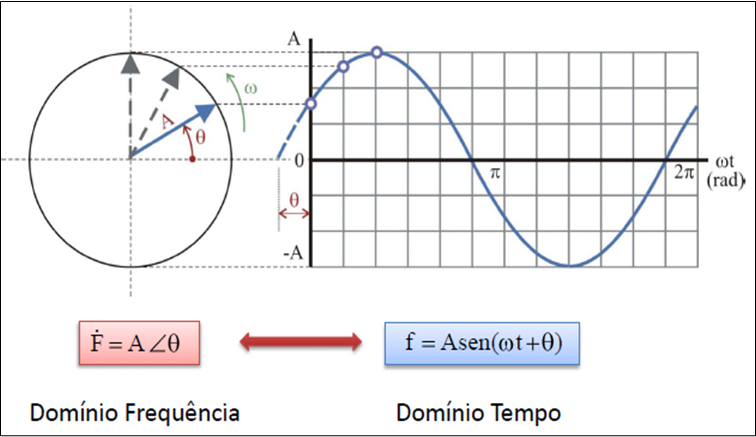
\includegraphics{aula2_12}\protect\caption{\label{fig:aula2_12}Fasores }
\end{centering}
\end{figure}
O que permite de fato levar a energia elétrica de um ponto para outro
muito distante nesse caso, aumentando a tensão é o transformador
de potencia.
O transformador de potencia é basicamente uma massa de ferro com um
enrolamento (enrola um fio em cada lado). A eficiência dos transformadores é
superior a 90\%, ou seja a energia perdida é pequena.
No transformador ideal, a tensão é gerada em função do fluxo magnético
variante no tempo, que é gerado em
função de uma corrente elétrica variante no tempo.
Se aplicarmos uma tensão de um lado, a tensão elétrica vai gerar uma
corrente que vai circular, essa corrente vai induzir um fluxo, esse
fluxo que passa no primário concatena com o secundário. Num transformador
ideal todo fluxo concatena. Quando aplicamos uma tensão, ela gera uma corrente, essa corrente vai produzir um fluxo que criará uma corrente do outro lado.
\begin{figure}[H]
\begin{centering}
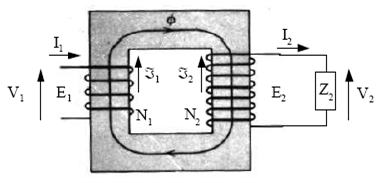
\includegraphics{aula2_13}\protect\caption{\label{fig:aula2_13}Transformador ideal de potência}
\end{centering}
\end{figure}

Matematicamente, da Lei de Faraday:
\begin{equation}\label{eq:lf}
\dot{\dot{V}_{1}=-N_{1}\frac{d\Phi}{dt}}
\end{equation}
\begin{equation}\label{eq:lf2}
\dot{\dot{V}_{2}=-N_{2}\frac{d\Phi}{dt}}
\end{equation}


onde,
$\dot{V_{i}}:$ Tensão (fasorial) no terminal i;

$\dot{I_{i}}:$ Tensão (fasorial) no terminal i;

$\dot{Ni}:$ Número de espiras no terminal i;

$\frac{d\Phi}{dt}$: Fluxo magnético variante no tempo.

Assim,

\begin{equation}\label{eq:lf2}
\frac{\dot{V}_{1}}{\dot{V}_{2}}=\frac{N_{1}}{N_{2}}=\alpha
\end{equation}

$\alpha$: Relação de transformação.

Se por exemplo colocarmos 10 espiras no primário e uma espira no secundário,eleva
a tensão no secundário para 10 vezes do primário. 
O análogo magnético (Figura \ref{fig:aula2_14}) do circuito elétrico do transformador é definido pelas equações abaixo:
\begin{equation}\label{eq:cet1}
\Im_{1}-\Im_{2}=\Re\cdot\Phi
\end{equation}

\begin{equation}\label{eq:cet2}
\Im_{1}=N_{1}\cdot\dot{I}_{1}
\end{equation}

\begin{equation}\label{eq:cet3}
\Im_{2}=N_{2}\cdot\dot{I}_{2}
\end{equation}


onde, 

$\Im_{i}$- Força magnetomotriz no terminal $i$ (A.e);

$\Phi$- Fluxo magnético induzido (Wb);

$\Re$- Relutância do transformador (A/Wb).

No transformador ideal, a relutância é nula. Assim:

\begin{equation}\label{eq:cet4}
N_{1}\cdot\dot{I}_{1}=N_{2}\cdot\dot{I}_{2}\rightarrow\frac{\dot{I}_{1}}{\dot{I}_{2}}=\frac{N_{1}}{N_{2}}=\frac{1}{\alpha}\rightarrow\dot{I}_{1}=\frac{1}{\alpha}\cdot\dot{I}_{2}
\end{equation}

\begin{figure}[H]
\begin{centering}
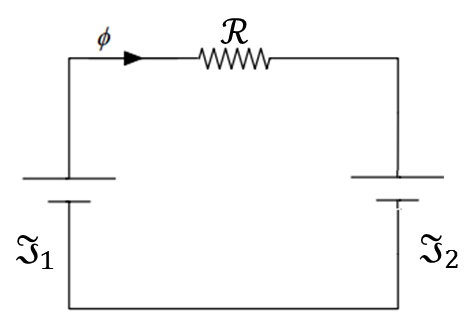
\includegraphics{aula2_14}\protect\caption{\label{fig:aula2_14}Circuito Magnético}
\end{centering}
\end{figure}

O transformador permite reduzir a corrente elétrica nas linhas
de transmissão aumentando a tensão. Neste caso, a energia elétrica
pode ser transmitida a grandes distâncias com menores perdas. 




\subsection{Evolução dos Sistemas Elétricos}


No nosso dia a dia, no trabalho, nos estudos, no lazer, sempre estamos fazendo uso da energia elétrica. A maioria das pessoas, no entanto, dão pouca importância para como esta energia chega até elas. Bom, o leite não vem da caixinha do supermercado, da mesma forma que a energia não chega magicamente às tomadas das nossas casas. Um sistema elétrico é algo muito complexo e que requer muito cuidado e planejamento. Imagine todo o Brasil interligado por uma rede de linhas de transmissão, com inúmeras unidades de geração e milhões de pessoas consumindo energia ao mesmo tempo. Quem controla tudo isso? Quem garante que a energia chegue às nossas casas? Se uma linha para de funcionar, como fazemos para levar a energia ao seu destino sem sobrecarregar demais as outras linhas?


Um sistema elétrico pode ser dividido em três partes: 1) Geração; 2) Transmissão; 3) Distribuição. A figura \ref{fig:sist} mostra um exemplo de um sistema elétrico. Tudo começa nas geradoras, que podem ser hidroelétricas, termoelétricas, torres eólicas, usinas nucleares e outras. A energia gerada vai para uma rede de transmissão básica que leva a energia até as estações de distribuição, para só então a energia chega ao consumidor final, nos famosos 110 (ou, à rigor, 127) e 220 volts que conhecemos. 

\begin{figure}[h]
\begin{centering}
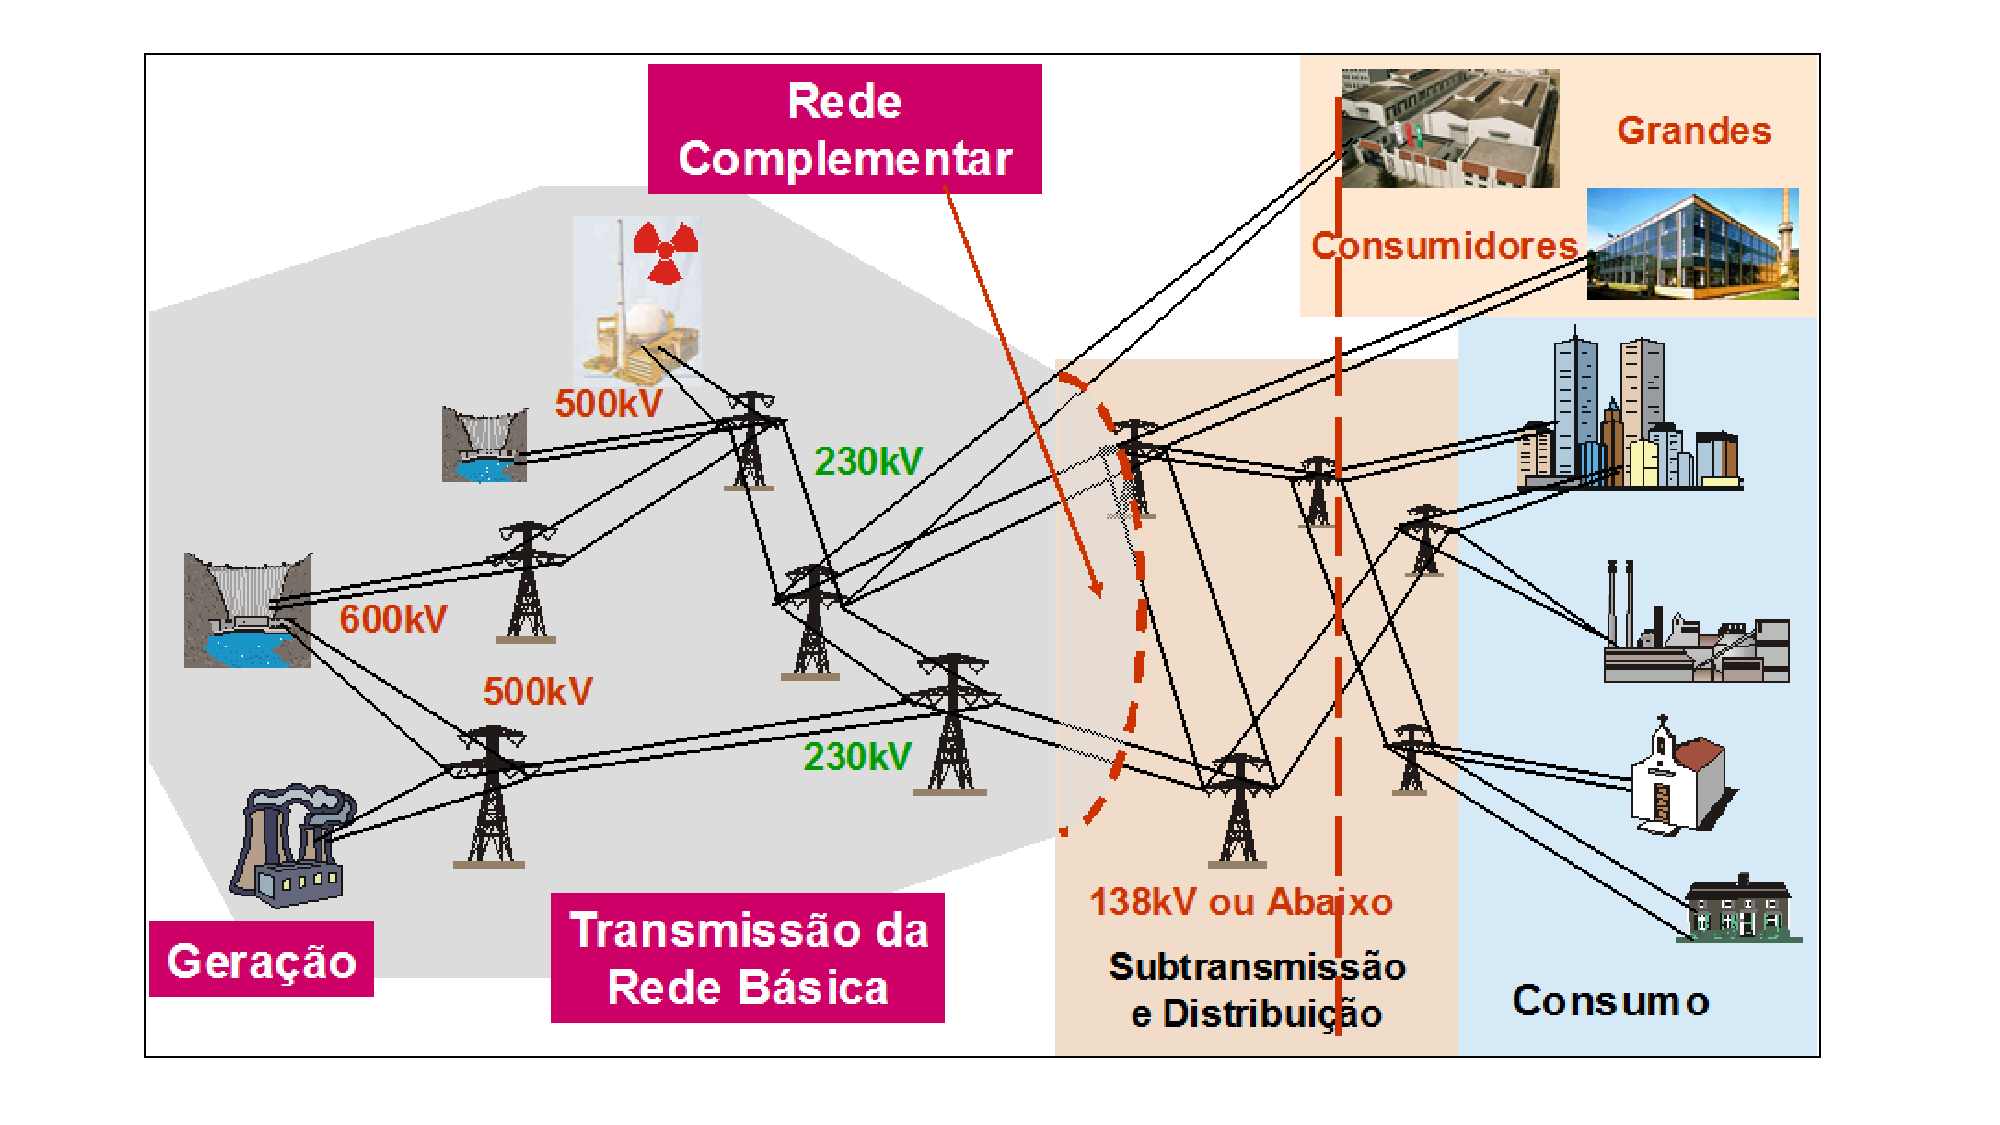
\includegraphics[scale=0.5]{anexos/figsist}
\par\end{centering}

\caption{\label{fig:sist}Representação de um sistema elétrico}
\end{figure}

\begin{figure}[h]
\begin{centering}
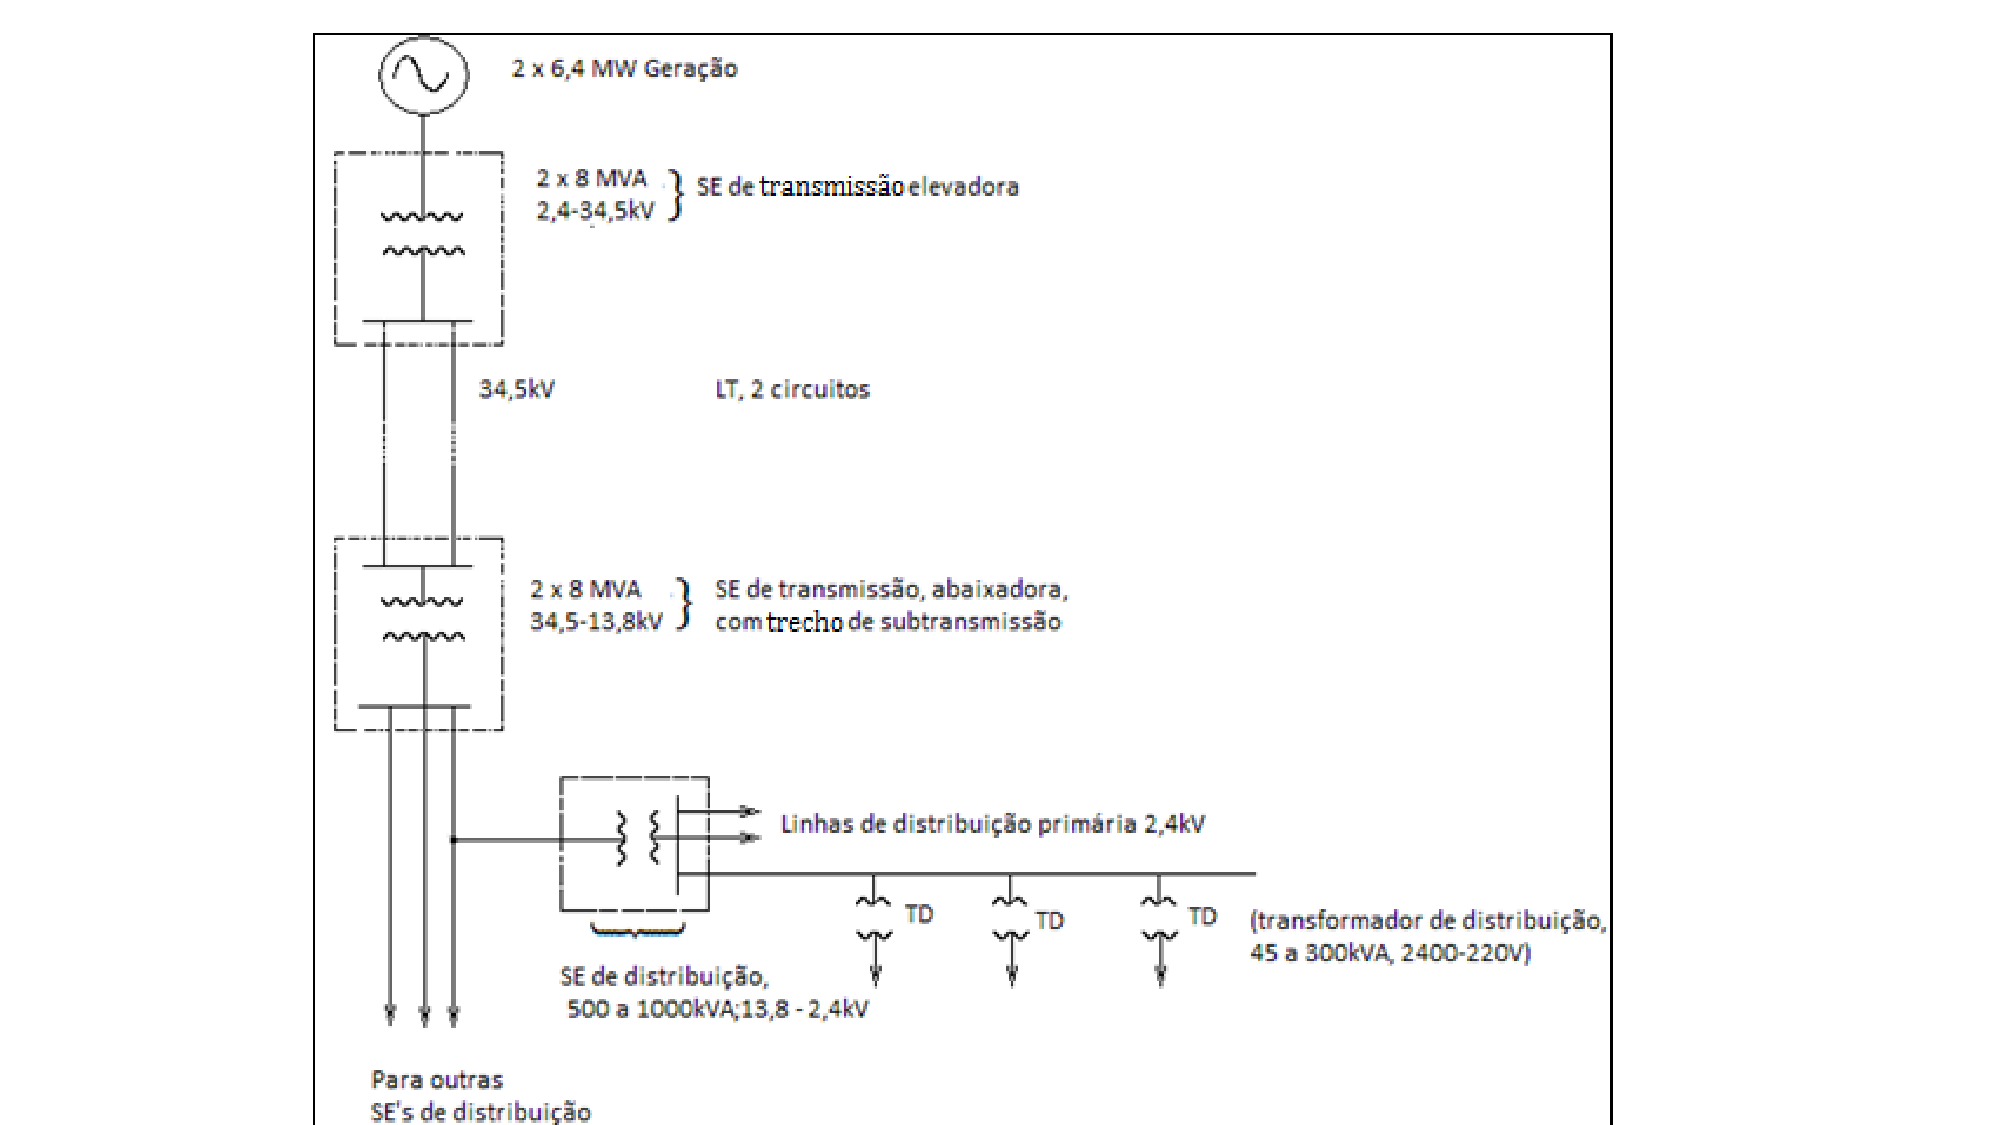
\includegraphics[scale=0.5]{anexos/figrede}
\par\end{centering}

\caption{\label{fig:rede}Sistema elétrico pequeno isolado}
\end{figure}

A figura \ref{fig:rede} mostra um pequeno sistema elétrico. As linhas e subestações no sistema são classificadas pela transformação no nível de tensão, e não a tensão no sistema como um todo. Pela figura podemos ver a tensão da geradora, que é aumentada em uma subestação. Em seguida, temos outra subestação que abaixa a tensão para 13.8kV até chegar subestação que leva às linhas de distribuição primárias, a 2.4kV. Estas linhas levam a energia até o poste, que tem um transformador que faz a energia chegar em nossas casas na tensão desejada, por exemplo, 220V. 

Já deu para notar que um sistema elétrico não é uma coisa simples, e que exige muita sincronia. Para controlar tudo isso existe o \textbf{Operador do Sistema}, que é uma entidade, que pode ou não pertencer ao governo, responsável por assegurar a funcionalidade do sistema elétrico. Dentre a funções do Operador do Sistema estão: garantir o funcionamento do mercado de energia (se ele existir), manter o sistema na frequência utilizada, assegurar que a demanda de energia será suprida, auxiliar no planejamento de expansão do sistema, minimizar custos de operação, entre outras. Estas funções podem variar de país para país.

Vamos falar agora sobre os diferentes custos de um sistema elétrico e como eles são classificados. Em primeiro lugar temos o custo de geração, que pode variar muito de gerador para gerador tanto em estrutura quando em valores absolutos. A construção de uma hidroelétrica é muito cara; entretanto, uma vez construída, a água não custa nada, ou seja, a usina não paga quase nada para funcionar. Em uma escala menor, o mesmo é valido para um parque eólico. No outro extremo estão as usinas térmicas; elas geralmente são baratas para serem construídas e podem ficar em qualquer lugar, o que reduz o custo de transmissão. No entanto, elas precisam queimar algum combustível como carvão ou gás natural, ou seja, apesar de serem baratas para construir, elas custam muito para operar. O primeiro caso que apresentamos foi o de geradores com um alto \textbf{custo fixo} e um baixo \textbf{custo variável}, no segundo caso esta relação se inverte. Além dos custos citados acima, fazem parte dos custos de geração possível custos ancilares, que podem ser custos da reserva de potência ativa, reativa, controle de frequência, controle de congestionamento do sistema, auto-restabelecimento, controle de tensão e outros.

Saindo da geração, vamos para os custos de transmissão e distribuição. Em primeiro lugar, quem arca com estes custos? Todos nós usamos linhas de transmissão, portanto o rateio destes custos pode ser algo complicado. Os custos de transmissão e distribuição são basicamente de construção e manutenção, no entanto, perdas de energia no sistema também são consideradas. É natural esperar que alguma energia será perdida no processo, e cabe ao planejador do sistema elétrico tentar minimizar estas perdas. 



\subsection{Modelagem dos Sistemas Elétricos}

Nesta seção, apresentaremos os três elementos utilizados para modelar as linhas de transmissão: resistores, indutores e capacitores. Veremos como a aplicação de uma tensão alternada se relaciona com a corrente gerada em cada um dos elementos. 

\subsubsection*{Resistores}


\begin{figure}
    \centering
    \begin{subfigure}[b]{0.3\textwidth}
        \centering
        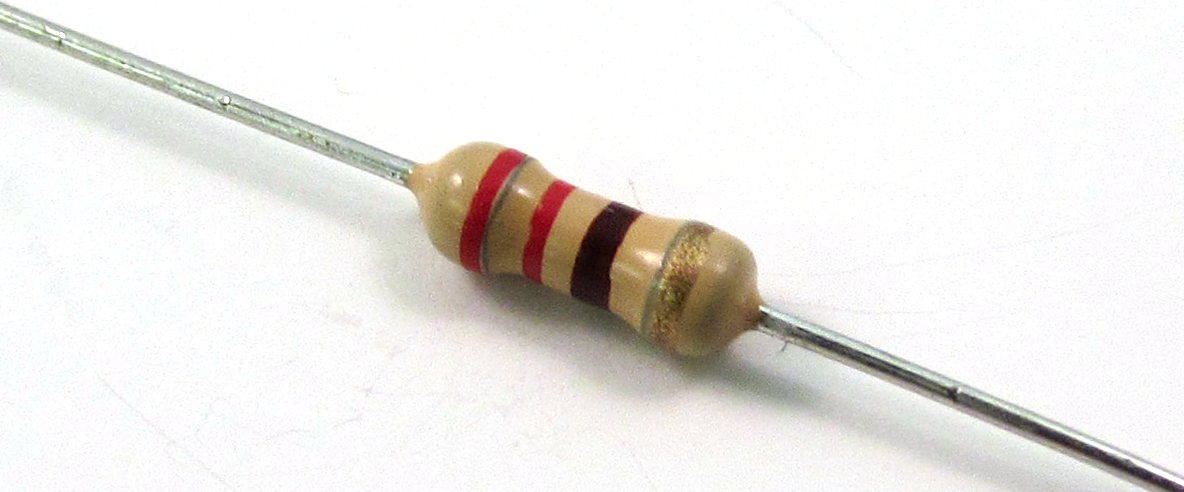
\includegraphics[width=\textwidth]{anexos/resistor.png}
        %\caption{$y=x$}
        %\label{fig:y equals x}
    \end{subfigure}
    \hspace{1cm}
    \begin{subfigure}[b]{0.3\textwidth}
        \centering
        \fbox{
            \begin{circuitikz} \draw
            (0,0) to[R, o-o, l=R] (0,2.5)
            ;
            \end{circuitikz}%\caption{$y=3sinx$}
            }
        %\label{fig:three sin x}
    \end{subfigure}
    

    \caption{À esquerda, um resistor real. À direita, a representação esquemática de um resistor.}
    \label{fig:three graphs}
\end{figure}


São equipamentos com características resistivas, como chuveiro elétrico
e aquecedor. As equações para a tensão ($V$) e corrente ($i$) em
função do tempo, assim como a representação com seus fasores correspondentes,
são exibidas a seguir:

\[
i(t)=\frac{V_{m}}{R}\mbox{\, sen}(wt+\phi)\qquad\longrightarrow\qquad\dot{I}=\frac{V_{m}}{R}\angle\phi^{\circ},
\]


\[
V(t)=V_{m}\mbox{\, sen}(wt+\phi)\qquad\longrightarrow\qquad\dot{V}=V_{m}\angle\phi^{\circ},
\]
em que $V_{m}$ é o valor máximo da tensão, ou seja, a sua amplitude.
A notação de fasor é uma forma simplificada de determinar a grandeza
no tempo, sem ter que especificar a função no sentido temporal, desde
que a frequência seja a mesma para todas as funções. No sistema elétrico utiliza-se comumente
frequências entre 50 e 60Hz. No Brasil, o padrão é de 60Hz. 

Para um resistor tem-se no domínio do tempo que 
\[
V(t)/i(t)=\frac{\frac{V_{m}}{R}\mbox{\, sen}(wt+\phi)}{V_{m}\mbox{\, sen}(wt+\phi)}=R
\]
 e no domínio da frequência que 
\[
\dot{V}/\dot{I}=R.
\]
 Assim, a fase que a corrente se encontra é exatamente a mesma da
tensão, como mostra a figura \ref{fig:fase-ct-resistor}. Como será
visto a seguir, isto não acontece para indutores e capacitores.



%\begin{center}
%\begin{table}[H]
%\begin{tabular}{ll}
%\multirow{2}{5cm}{  \begin{circuitikz} \draw
%    (0,0) to[R, o-o, l=R] (0,3)
%    ;
%    \end{circuitikz}}    & $e = E_m\text{sen}(wt+\phi)$ \\
%                                        & $i=\dfrac{E_m}{R}\text{sen}(wt+\phi)$ \\
%\end{tabular}
%\end{table}
%\end{center}

%\begin{figure}[H]
%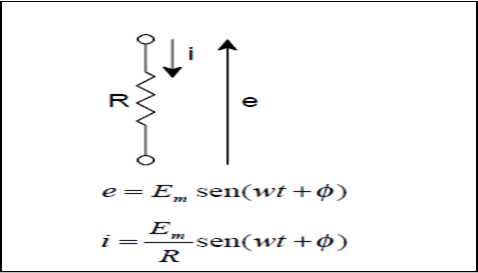
\includegraphics{anexos/aula2_1.png}\protect\caption{Resistores}
%\end{figure}




%Figura resistor
\begin{figure}[H]
\begin{center}
\fbox {
    \begin{tikzpicture}[domain=0:4]
        \draw[very thin,color=gray] (-0.1,-2.1) grid (3.9,2.1);
        \draw[->] (-0.2,0) -- (4.2,0) node[right] {$t$};
        \draw[->] (0,-2.2) -- (0,2.2) node[above] {};
        \draw[smooth, color=blue] plot[id=sin] function{sin(5*x)} 
            node[right] {$i(t)=\frac{V_{m}}{R}\mbox{\,\ sen}(wt+\phi)$};
        \draw[smooth, color=orange] plot[id=exp] function{2*sin(5*x)} 
            node[right] {$V=V_{m}\mbox{\, sen}(wt+\phi)$};
    \end{tikzpicture}
    }
\caption{\label{fig:fase-ct-resistor}Corrente e tensão oscilam na mesma fase no resistor}
\end{center}
\end{figure}


\subsubsection*{Indutores}

% Figura Indutor
\begin{figure}
    \centering
    \begin{subfigure}[b]{0.3\textwidth}
        \centering
        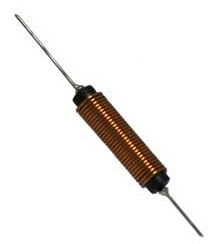
\includegraphics[width=\textwidth]{anexos/indutor.png}
        %\caption{$y=x$}
        %\label{fig:y equals x}
    \end{subfigure}
    \hspace{1cm}
    \begin{subfigure}[b]{0.3\textwidth}
        \centering
        \fbox{
            \begin{circuitikz} \draw
            (0,0) to[cute inductor, o-o, l=L] (0,2.5)
            ;
            \end{circuitikz}%\caption{$y=3sinx$}
            }
        %\label{fig:three sin x}
    \end{subfigure}
    \caption{À esquerda, um indutor real. À direita, a representação esquemática de um indutor.}
    \label{fig:three graphs}
\end{figure}


Quando a corrente passa por equipamentos como um motor elétrico ou
um transformador (elementos indutivos), a fase da corrente se atrasa
com relação à tensão. Sendo a diferença de potencial num indutor medido
como $V=L\,\frac{di}{dt}$, em que $L$ é a indutância, apresentamos a seguir o cálculo das relações
entre corrente e tensão a seguir:

\[
i(t)=\frac{V_{m}}{R}\mbox{\,\ sen}(wt+\phi)\qquad\longrightarrow\qquad\dot{I}=I_{m}\angle\phi^{\circ},
\]


\[
V(t)=L\,\frac{di}{dt}=wLI_{m}\mbox{cos}(wt+\phi)=wLI_{m}\mbox{sen}(wt+\phi+90)\qquad\longrightarrow\qquad\dot{V}=wLI_{m}\angle\phi+90^{\circ},
\]


\begin{equation}
\frac{\dot{V}}{\dot{I}}=\frac{wLI_{m}\angle\phi+90^{\circ}}{I_{m}\angle\phi^{\circ}}=wL\angle90^{\circ}.\label{eq:fase-v-i}
\end{equation}
Assim, conforme visto nas equações acima, a fase da corrente num indutor
se atrasa em $90^{\circ}$ com relação à tensão. A forma regular da
expressão \ref{eq:fase-v-i} pode ser escrita também como um número
complexo num plano de Argand-Gauss: 
\[
\frac{\dot{V}}{\dot{I}}=jwL.
\]
Este plano é similar ao plano cartesiano, com a diferença que no eixo horizontal está a parte real $a$ do número $a+bj$ e no eixo vertical a parte imaginária $b.$ Nota-se que utiliza-se a letra $j$ para representar $\sqrt{-1}$, pois a letra $i$ já é usada para denominar a corrente. Denomina-se como \textbf{reatância indutiva} ($X_L$)o valor equivalente de resistência que o indutor provoca no sistema. 



% Figura senoide Indutor
\begin{figure}[H]
\begin{center}
\fbox {
    \begin{tikzpicture}[domain=0:4]
        \draw[very thin,color=gray] (-0.1,-2.1) grid (3.9,2.1);
        \draw[->] (-0.2,0) -- (4.2,0) node[right] {$t$};
        \draw[->] (0,-2.2) -- (0,2.2) node[above] {};
        \draw[smooth, color=blue] plot[id=sin] function{sin(6*x)} 
            node[right] {$\dot{I}=I_{m}\angle\phi^{\circ}$};
        \draw[smooth, color=orange] plot[id=exp] function{2*sin(6*x+90)} 
            node[right] {$\dot{V}=wLI_{m}\angle\phi+90^{\circ}$};
    \end{tikzpicture}
    }
\caption{\label{fig:fase-ct-indutor}Corrente é atrasada em 90º com relação à tensão num indutor}
\end{center}
\end{figure}


\subsubsection*{Capacitores}

%Figura capacitor 
\begin{figure}
    \centering
    \begin{subfigure}[b]{0.3\textwidth}
        \centering
        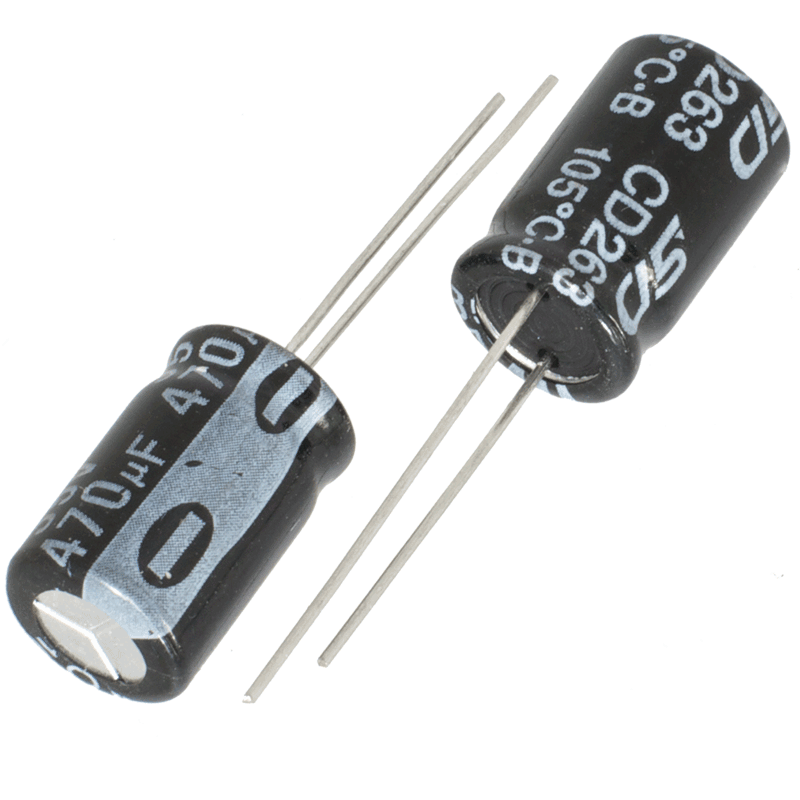
\includegraphics[width=\textwidth]{anexos/capacitor.png}
        %\caption{$y=x$}
        %\label{fig:y equals x}
    \end{subfigure}
    \hspace{1cm}
    \begin{subfigure}[b]{0.3\textwidth}
        \centering
        \fbox{
            \begin{circuitikz} \draw
            (0,0) to[capacitor, o-o, l=C] (0,2.5)
            ;
            \end{circuitikz}%\caption{$y=3sinx$}
            }
        %\label{fig:three sin x}
    \end{subfigure}
    \caption{À esquerda, um resistor real. À direita, a representação esquemática de um resistor.}
    \label{fig:three graphs}
\end{figure}


O único elemento capacitivo numa rede são os próprios bancos de capacitores.
Ele é utilizado principalmente para regulagem da tensão e fator de
potência. Sendo $C$ a capacitância do capacitor em questão, temos
que:

\[
V(t)=V_{m}\mbox{\,\ sen}(wt+\phi)\qquad\longrightarrow\qquad\dot{V}=V_{m}\angle\phi^{\circ},
\]


\[
i(t)=C\,\frac{dV}{dt}=wCV_{m}\mbox{cos}(wt+\phi)=wCV_{m}\,\mbox{sen}(wt+\phi+90)\qquad\longrightarrow\qquad\dot{I}=wCV_{m}\angle\phi+90^{\circ},
\]


\[
\frac{\dot{V}}{\dot{I}}=\frac{V_{m}\angle\phi^{\circ}}{wCV_{m}\angle\phi+90^{\circ}}=\frac{1}{wC\angle90^{\circ}}.
\]
Passando para a forma retangular através de números complexos, temos que
\[
\frac{\dot{V}}{\dot{I}}=\frac{1}{jwC}=\frac{-j}{wC}.
\]
Assim, a reatância capacitiva é dada por $X_{C}=\frac{1}{wC}$. 

% Figura capacitor
\begin{figure}[H]
\begin{center}
\fbox {
    \begin{tikzpicture}[domain=0:4]
        \draw[very thin,color=gray] (-0.1,-2.1) grid (3.9,2.1);
        \draw[->] (-0.2,0) -- (4.2,0) node[right] {$t$};
        \draw[->] (0,-2.2) -- (0,2.2) node[above] {};
        \draw[smooth, color=blue] plot[id=sin] function{sin(5*x)} 
            node[right] {$\dot{I}=I_{m}\angle\phi^{\circ}$};
        \draw[smooth, color=orange] plot[id=exp] function{2*sin(5*x-90)} 
            node[right] {$\dot{V}=wLI_{m}\angle\phi+90^{\circ}$};
    \end{tikzpicture}
    }
\caption{\label{fig:fase-ct-indutor}Corrente é adiantada em 90º com relação à tensão num capacitor}
\end{center}
\end{figure}

\subsubsection*{Linhas de transmissão}

Para modelar as linhas de transmissão, verifica-se qual a impedância do sistema. A impedância é dada pela combinação da resistência, reatância capacitiva e reatância indutiva.

% Figura corrente alternada
%\begin{figure}[H]
%\begin{center}
%\fbox {
%    \begin{tikzpicture}[domain=0:4]
%        \draw[very thin,color=gray] (-0.1,-2.1) grid (3.9,2.1);
%        \draw[->] (-0.2,0) -- (4.2,0) node[right] {$t$};
%        \draw[->] (0,-2.2) -- (0,2.2) node[above] {$V$};
%        \draw[smooth, color=blue] plot[id=sin] function{sin(5*x)} 
%            node[right] {Corrente alternada};
%    \end{tikzpicture}
%    }
%\caption{\label{fig:fase-ct-indutor}Corrente é atrasada em 90º com relação à tensão num indutor}
%\end{center}
%\end{figure}
%
%
%
%
%% Figura corrente contínua
%\begin{figure}[H]
%\begin{center}
%\fbox {
%    \begin{tikzpicture}[domain=0:4]
%        \draw[very thin,color=gray] (-0.1,-0.1) grid (3.9,3.9);
%        \draw[->] (-0.2,0) -- (4.2,0) node[right] {$i$};
%        \draw[->] (0,-0.2) -- (0,4.2) node[above] {$V$};
%        \draw[smooth, color=blue] plot[id=sin] function{2} 
%            node[right] {Corrente contínua};
%    \end{tikzpicture}
%    }
%\caption{\label{fig:fase-ct-indutor}Corrente é atrasada em 90º com relação à tensão num indutor}
%\end{center}
%\end{figure}
%
%
%
%\begin{center}
%\begin{tikzpicture}
%    \begin{axis}[domain=0:1,legend pos=outer north east]
%    \addplot[smooth] {2*sin(20*deg(x))}; 
%    \addplot[smooth, red] {sin(20*deg(x))}; 
%    \legend{$i=\frac{E_{m}}{R}\mbox{\,\ sen}(wt+\phi)$,$
%e=E_{m}\mbox{\, sen}(wt+\phi)$}
%    \end{axis}
%\end{tikzpicture}
%\end{center}

\section{Aula 3}

\subsection{Método Newton-Raphson}
O Método Newton-Raphson tem como objetivo estimar as raízes de uma
função, escolhendo uma aproximação inicial para esta e após a escolha
calcular a equação tangente da função neste ponto e a interseção dela
com o eixo das abcissas, a fim de encontrar uma melhor aproximação
para a raiz. O processo é repetido, criando assim um método iterativo
para encontrar a raiz da função. O algoritmo para o caso univariado é apresentado a seguir.


\begin{framed} %Box algoritmo
    \textbf{O algoritmo de Newton-Raphson}
    
    \begin{enumerate}
    \item Arbitrar uma condição inicial $(x_{i}-x_{0})$ e fixar $i=0$;
    
    \item Calcular $f(x_{i})$ e verificar a convergência. Se $|f(x_{i})|\leq \varepsilon$, então parar.
    
    \item Linearizar a função em torno de $(f(x_{i}),x_{i})$ e igualar a função
    a zero para estabelecer o passo $(\triangle x_{i}=x_{i+1}-x_{i})$
    e novo ponto $(x_{i+1})$.
    $$f(x)=f(x_{i})+f^{'}(x_{i})\cdot(x_{i+1}-x_{i})=0$$
    $$x_{i+1}=x_{i}-\frac{f(x_{i})}{f^{'}(x_{i})}$$
    
    \item Fazer $i=i+1$e voltar ao passo 2.
    
    \end{enumerate}
    
    Uma representação  gráfica do algoritmo é mostrada na figura \ref{fig:aula3_7}.
    
\end{framed}

\begin{figure}[H]
\begin{centering}
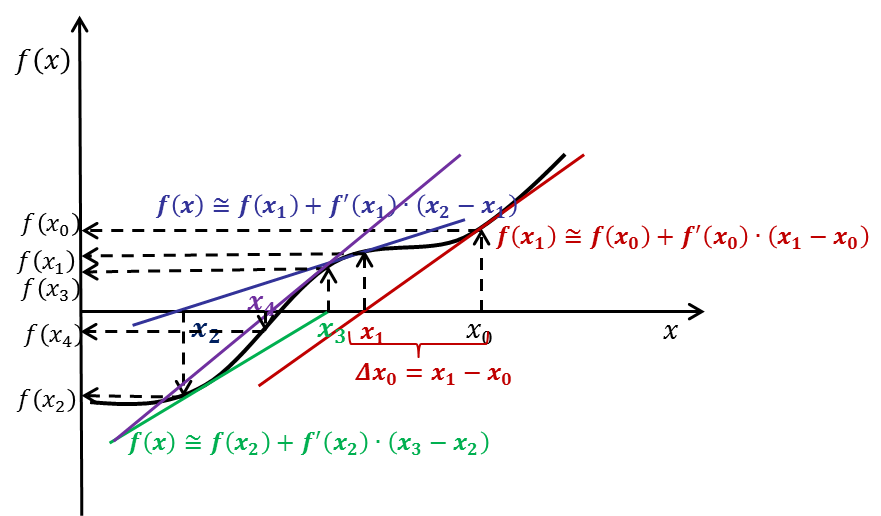
\includegraphics[scale=0.8]{aula3_7}\protect\caption{\label{fig:aula3_7} Algoritmo do Método de Newton  }
\end{centering}
\end{figure}

O método de Newton se baseia na expansão por \textbf{séries de Taylor} que, por definição, é uma forma de aproximar uma função $f$ ao redor de um ponto $x_{0}$ através da soma de polinômios.
Se uma função e suas derivadas até a ordem $n+1$ forem contínuas
em um intervalo contendo $x$ e $x_{0}$, então a expansão de Taylor é dada por: 

\[
f(x)=f(x_{0})+f^{'}(x_{0})\cdot(x-x_{0})+\frac{1}{2!}\cdot f^{''}(x_{0})\cdot(x-x_{0})^{2}+...+\frac{1}{n!}\cdot f^{(n)}(x_{0})\cdot(x-x_{0})^{n}+R_{n}.
\]

A representação gráfica dos termos da série de Taylor é dada pela Figura \ref{fig:aula3_2}.

\begin{figure}[H]
\begin{centering}
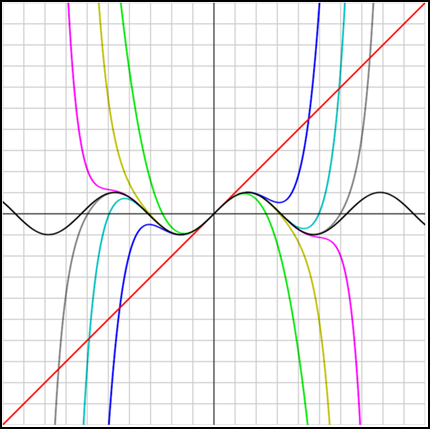
\includegraphics{aula3_2}\protect\caption{\label{fig:aula3_2} Série de Taylor }
\end{centering}
\end{figure}


Truncando a série no termo de 1ª ordem (ou seja, descartando todos os termos de ordem superior a 2), temos: 
\[
	f(x)=f(x_{0})+f^{'}(x_{0})\cdot(x-x_{0}).
\]
Tomando a expansão em torno de $x_0$, a interseção desta reta com o eixo das abcissas é encontrada em $x'$ resolvendo a equação: 
\[
	x' = x_0 - \dfrac{f(x_0)}{f'(x_0)} .
\]
Assim, o algoritmo funciona tomando o $x'$ como o valor de $x_{i+1}$ depois da $i$-ésima iteração, e continuando o algoritmo até atender um critério de parada. 
%  Como queremos (escolha inicial):
%\[
%x_{1}=x_{0}-\frac{f(x_{0})}{f^{'}(x_{0})},
%\]


\begin{exemplo}
Seja a função $f(x)=x^{2}-6\cdot\sin(x)$ com $x\in[1;3]$. Uma maneira de se encontrar a solução é plotar a função e procurar a solução visualmente, conforme na figura \ref{fig:aula3_1}. 
\begin{figure}[H]
\begin{centering}
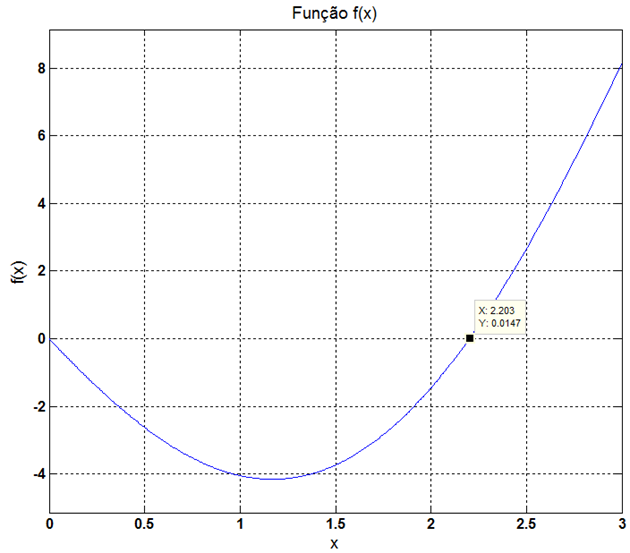
\includegraphics{aula3_1}\protect\caption{\label{fig:aula3_1} Solução gráfica }
\end{centering}
\end{figure}

Considerando
uma escolha inicial de $x_{0}=2,5$, vamos utilizar o método de Newton-Raphson para aproximar uma raiz da função $f$ com uma tolerância $\varepsilon=0,05$.  Para a primeira iteração, devemos procurar
\[
x_{1}=x_{0}-\frac{f(x_{0})}{f^{'}(x_{0})},
\]
A função avaliada em $x_{0}=2,5$, com as derivadas em torno do ponto resultam
em:
\begin{eqnarray*}
f(x_{0}) & = & f(2,5)=2,6592 \\
f^{'}(x_{0}) & = & f^{'}(2,5)=9,8069
\end{eqnarray*}
Assim, substituindo os valores na equação para $x_{0}=2,5$, obtém-se uma aproximação da função $f$ em torno de $x_0$:
\[
f(x)\cong2,66+9,81\cdot(x-2,5).
\]

\begin{figure}[H]
\begin{centering}
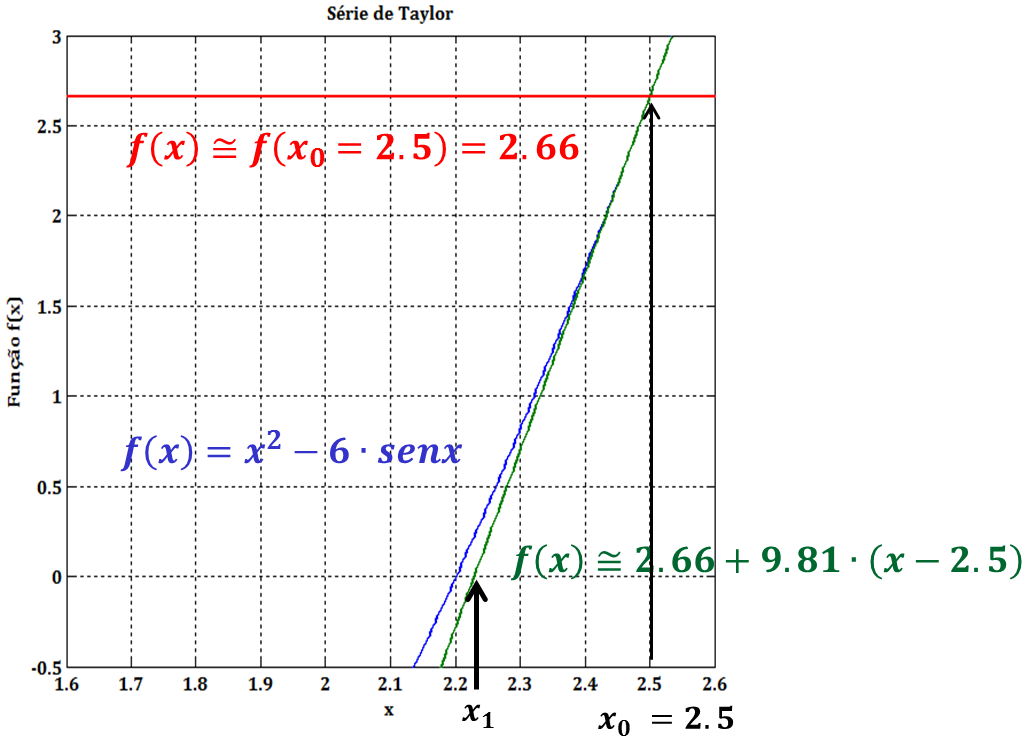
\includegraphics[scale=0.8]{aula3_3}\protect\caption{\label{fig:aula3_3} Gráfico  $x_{0}=2,5$  }
\end{centering}
\end{figure}
Na figura \ref{fig:aula3_3}, a reta azul representa a função original do problema e a verde é a expansão em série de Taylor linearizada no polinômio de primeira ordem. O ponto $x_1$ é encontrado através da expressão
\[
x_{1}=2,5-\frac{2,6562}{9,8069}\cong2,23.
\]
Usando o ponto $x_{1}=2,23$ na função $f(x)=x^{2}-6\cdot\sin(x)$:

\[
| f(2,23)|=|2,23^{2}-6\cdot\sin(2,23)|=|0,23|>0,05
\]
A solução $x_{1}=2,23$ não satisfaz a restrição do problema. Utilizamos o $x_1$ para a próxima iteração (ver figura \ref{fig:aula3_4}), temos que 
\begin{figure}[H]
\begin{centering}
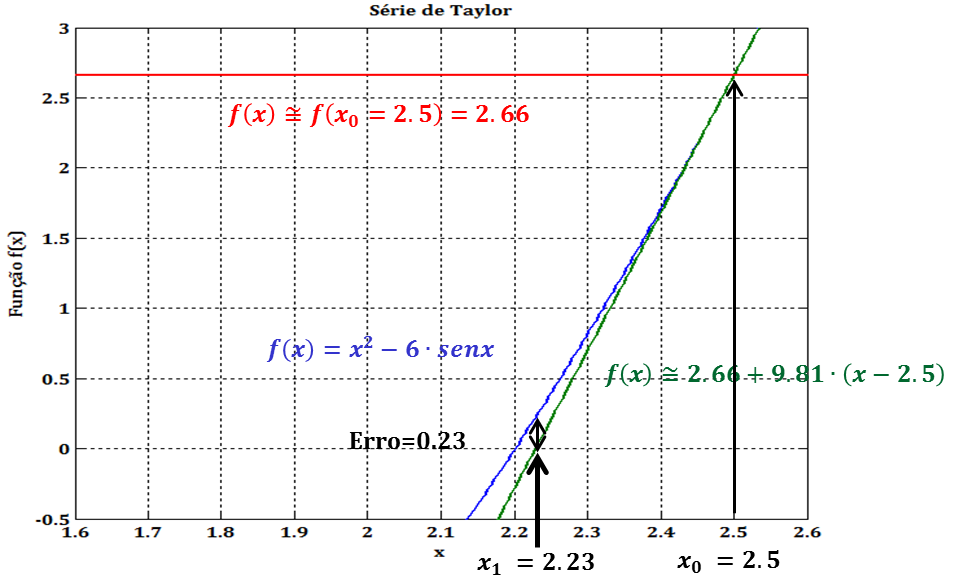
\includegraphics[scale=0.8]{aula3_4}\protect\caption{\label{fig:aula3_4} Gráfico com a tolerância de $x_{0}=2,5$  }
\end{centering}
\end{figure}
O ponto $x_{1}=2,23$ é o ponto de partida para a segunda iteração.
Linearizando em torno de $x_{1}=2,23$ (Gráfico \ref{fig:aula3_5}):
\begin{figure}[H]
\begin{centering}
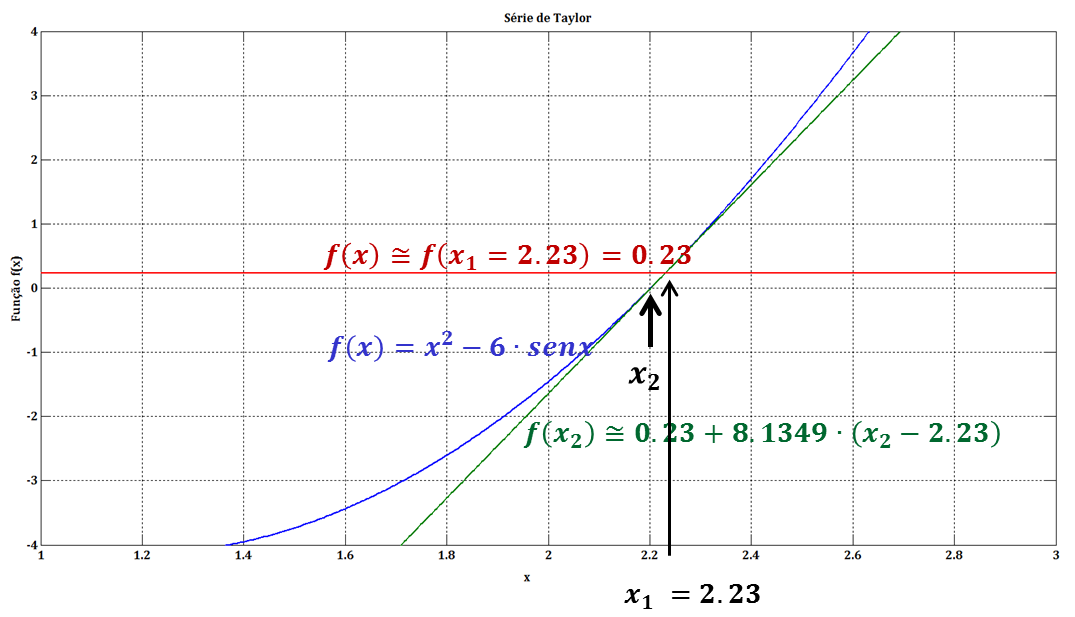
\includegraphics[scale=0.8]{aula3_5}\protect\caption{\label{fig:aula3_5} Linearização no ponto $x_{1}=2,23$  }
\end{centering}
\end{figure}
$$f(x_{1})=f(2,23)=0,23,$$
$$f^{'}(x_{1})=f^{'}(2,23)=8,1319,$$
$$x_{2}=x_{1}-\frac{f(x_{1})}{f^{'}(x_{1})}.$$
Assim, temos que:
$$f(x)\cong0,23+8,1349\cdot(x_{2}-2,23)$$
$$x_{2}=2,23 - \frac{0,23}{8,81349} \cong 2,20.$$
Usando o ponto $(x_{2}=2,2)$ na função $f(x_{2}^{2})=x_{2}^{2}-6\cdot\sin x_{2}$:
\[
	|f(2,2)|=|2,2^{2}-6\cdot\sin(2,2)|=|0,03|<0,05.
\]
Portanto, $x_{2}=2,2$ satisfaz a solução do problema. Caso seja necessário
encontrar uma tolerância menor que $0,03$ o processo deve ser repetido.
Graficamente, para $x_{1}=2,23$:
\begin{figure}[H]
\begin{centering}
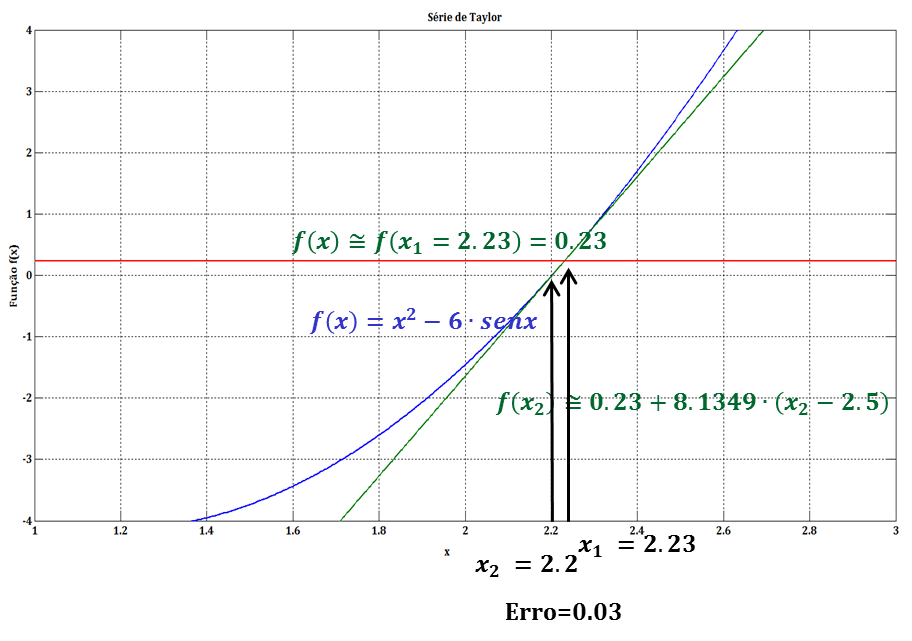
\includegraphics[scale=0.8]{aula3_6}\protect\caption{\label{fig:aula3_6} Gráfico para $x_{1}=2,23$  }
\end{centering}
\end{figure}







\begin{figure}[H]
\begin{centering}
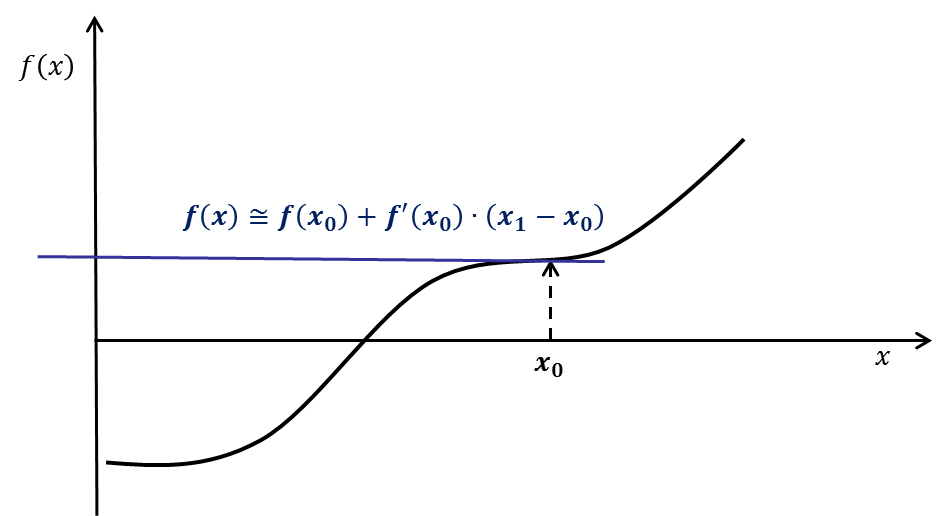
\includegraphics[scale=0.8]{aula3_8}\protect\caption{\label{fig:aula3_8} Escolha inicial  }
\end{centering}
\end{figure}

\end{exemplo}


Ao aplicar o método de Newton, deve-se tomar cuidado. O método é eficiente quando o ponto inicial $x_0$ é relativamente próximo da solução, mas pode ser ruim quando o chute inicial não for bom. Observe a figura \ref{fig:aula3_8}. A derivada avaliada em $x_0$ é 0, assim $x_{1}=x_{0}-\frac{f(x_{0})}{f^{'}(x_{0})}$; como o termo $\frac{f(x_{0})}{f^{'}(x_{0})}$ vai para infinito, a solução nunca seria encontrada. 

O método de Newton é adequado para o problema do fluxo de potência. Como as soluções do problema ($V$ e $\theta$) normalmente são próximas de 1 (um) pu e 0 (zero) radianos, então a escolha da solução inicial será normalmente adequada.

A diferença do fluxo de potencial do exemplo anterior é que temos
um conjunto de funções para resolver.

Já o \textbf{método de Newton aplicado ao caso multivariável} deve considerar:
\[
\begin{matrix} 
F(x)= & [f_{ 1 } & { f }_{ 2 } & ... & { f }_{ n }{ ] }^{ T } 
\end{matrix}
\begin{matrix} 
x= & [x_{ 1 } & { x }_{ 2 } & ... & { x }_{ n }{ ] }^{ T } 
\end{matrix}
\]
Sendo que, $F(x)$ representa um vetor de funções e $x$ é um conjunto
de variáveis.


\begin{framed} %Box algoritmo multivariado
    \textbf{O algoritmo de Newton-Raphson multivariado}
    \begin{enumerate}
    \item Arbitrar uma condição inicial $(x^{(i)}=x^{(0)})$ e fixar $i=0$;
    
    \item Calcular $F(x^{(i)})$ e verificar a convergência. Se $\max| F(x^{(i)})|\leq \varepsilon,$ então parar.
    
    \item Linearizar a função em torno de $(F(x^{(i)}),x^{(i)})$ e igualar
    a função a zero para estabelecer o passo $(\triangle x^{(i)}=x^{(i+1)}-x_{i}^{(i)})$
    e novo ponto $(x^{(i+1)})$.
    Para o caso de apenas uma variável, temos que:
    \[
    f(x)=f(x_{i})+f^{'}(x_{i})\cdot(x_{i+1}-x_{i})=0
    \]
    \[
    x_{i+1}=x_{i}-\frac{f(x_{i})}{f^{'}(x_{i})}.
    \]
    Já para o caso multivariado, temos que:
    \[
    F(x)=F(x^{(i)})+[J(x^{(i)})]\cdot(x^{(i+1)}-x^{(i)})=0
    \]
    \[
    x^{(i+1)}=x^{(i)}-[J(x^{(i)})]^{-1}\cdot F(x^{(i)}),
    \]
    sendo que $J(x^{(i)})=[\frac{\partial F(x)}{\partial x}]$ é a matriz jacobiana
    de derivadas de $F(x)$ com relação à $x$.
    \item Fazer $i=i+1$ e voltar ao passo 2.
    \end{enumerate}
    
    
\end{framed}


Para calcular a matriz jacobiana, primeiro cria-se um vetor $F$ com as $n$ funções em questão:
\[
\begin{matrix} 
F(x)= & [f_{ 1 } & { f }_{ 2 } & \dots & { f }_{ n }{ ] }^{ T }, 
\end{matrix}
\]
em que $\begin{matrix} 
x= & [x_{ 1 } & { x }_{ 2 } & \dots & { x }_{ n }{ ] }^{ T } 
\end{matrix}$. A matriz jacobiana é dada pelas derivadas cruzadas da função $F$:
\[
	\left[J(x^{(i)})\right]=\left[\frac{\partial F(x)}{\partial x}\right]=\left[\begin{array}{ccc}
	\frac{\partial f_{1}}{\partial x_{1}} & \cdots & \frac{\partial f_{1}}{\partial x_{m}}\\
	\vdots & \ddots & \vdots\\
	\frac{\partial f_{n}}{\partial x_{1}} & \vdots & \frac{\partial f_{n}}{\partial x_{m}}
	\end{array}\right]
\]
As equações básicas do subproblema 1 (barras PQ+PV) a serem solucionadas
são:
\[
P_{k}=V_{k}\sum_{m=1}^{n}V_{m}(G_{km}\cos\theta_{km}+B_{km}\sin\theta_{km}),\forall k\in\{\Omega_{PQ},\Omega_{PV}\},
\]
\[
Qk=V_{k}\sum_{m=1}^{n}V_{m}(G_{km}\sin\theta_{km}+B_{km}\cos\theta_{km}),\forall k\in\{\Omega_{PQ}\},
\]
onde, $\Omega_{PQ}$ são os conjuntos de barras do tipo PQ, $\Omega_{PV}$ são os conjuntos de barras do tipo PV. Considerando que para algumas barras os valores de P e Q são conhecidos, os ``resíduos'' de potência são dados por:
\[
\Delta P_{k}=P_{k}^{(especificado)}-P_{k}^{(calculado)}(V,\theta),\forall k\in\{\Omega_{PQ},\Omega_{PV}\},
\]
\[
\Delta Q_{k}=Q_{k}^{(especificado)}-Q_{k}^{(calculado)}(V,\theta),\forall k\in\{\Omega_{PQ}\},
\]
em que $P_{k}^{(especificado)}$ são os valores de potência ativa (conhecidos) na
barra $k$ e $Q_{k}^{(especificado)}$ são os valores de potência ativa(conhecido) na barra $k$.

Neste caso: \todo{como apresentar isso aqui?}
\[
	\begin{matrix}
	F(\Delta { P },\Delta Q)= & [\Delta { P }_{ 1 } & \Delta { P }_{ 2 } & ... & \Delta { P }_{ n }^{ \quad } & \Delta { Q }_{ 1 } & \Delta { Q }_{ 2 } & \dots & { \Delta { Q } }_{ n }] 
	\end{matrix}
\]
\[
	\begin{matrix} 
	x= & [\theta _{ 1 } & \theta _{ 2 } & ... & \theta _{ n }^{ \quad } & V_{ 1 } & V_{ 2 } & \dots & { V }_{ n }] 
	\end{matrix}
\]

A matriz Jacobiana associada ao problema proposto é apresentada na Figura \ref{fig:aula3_9}.


\begin{figure}[H]
\begin{centering}
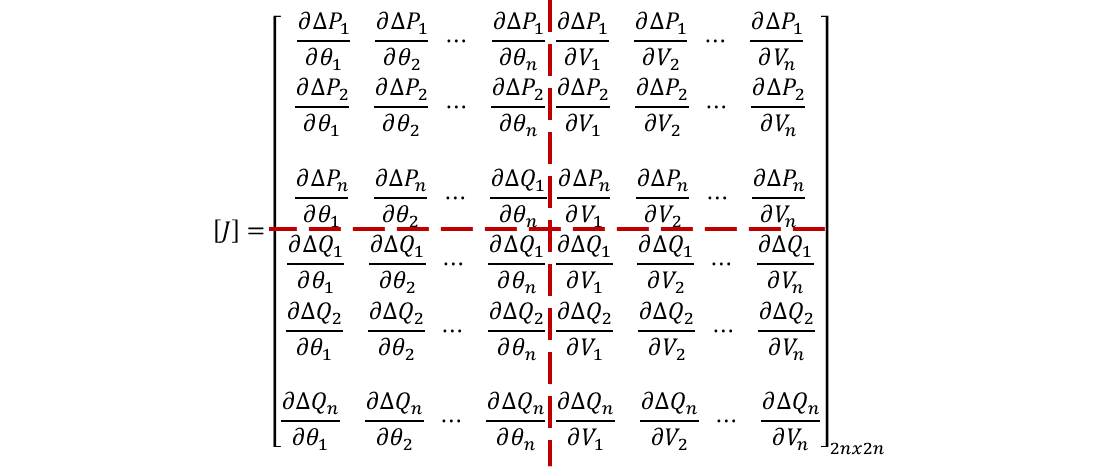
\includegraphics{aula3_9}\protect\caption{\label{fig:aula3_9} Matriz jacobiana  }
\end{centering}
\end{figure}

A seguir, calculamos os elementos da matriz jacobiana:
\[
\frac{\partial\triangle P_{k}}{\partial\theta_{m}}=\frac{\partial(P_{k}^{(especificado)}-P_{k}^{(calculado)})}{\partial\theta_{m}}=-\frac{\partial P_{k}^{(calculado)}}{\partial\theta_{m}},\qquad\forall m,k
\]
\[
\frac{\partial\triangle P_{k}}{\partial V_{m}}=\frac{\partial(P_{k}^{(especificado)}-P_{k}^{(calculado)})}{\partial V_{m}}=-\frac{\partial P_{k}^{(calculado)}}{\partial V_{m}},\qquad\forall m,k
\]
\[
\frac{\partial\triangle Q_{k}}{\partial\theta_{m}}=\frac{\partial(Q_{k}^{(especificado)}-Q_{k}^{(calculado)})}{\partial\theta_{m}}=-\frac{\partial Q_{k}^{(calculado)}}{\partial\theta_{m}},\qquad\forall m,k
\]
\[
\frac{\partial\triangle Q_{k}}{\partial V_{m}}=\frac{\partial(Q_{k}^{(especificado)}-Q_{k}^{(calculado)})}{\partial V_{m}}=-\frac{\partial Q_{k}^{(calculado)}}{\partial V_{m}},\qquad\forall m,k
\]


Como $P_{k}^{(especificado)}$ e
$Q_{k}^{(especificado)}$ são constantes a matriz Jacobiana pode ser reescrita como apresentamos a seguir:
\[
[J]=- \begin{bmatrix} \frac { \partial { P }^{ (calculado) } }{ \partial \theta } & \frac { \partial { P }^{ (calculado) } }{ \partial V } \\ \frac { \partial { Q }^{ (calculado) } }{ \partial \theta } & \frac { \partial { Q }^{ (calculado) } }{ \partial V } \end{bmatrix}_{ 2n \times 2n }=-{ \begin{bmatrix} H & N \\ M & L \end{bmatrix} }_{ 2n \times 2n }
\]
\[
H_{km}=\frac{\partial P_{k}^{(calculado)}}{\partial\theta_{m}}=V_{k}\cdot V_{m}\cdot\{G_{km}\cdot\sin(\theta_{km})-B_{km}\cdot\cos(\theta_{km})\},\forall k\neq m
\]


\[
H_{km}=\frac{\partial P_{k}^{(calculado)}}{\partial\theta_{k}}=-V_{k}^{2}\cdot B_{kk}-V_{k}\cdot\left[\sum_{m\in\Omega_{k}}V_{m}\cdot\{G_{km}\cdot\sin(\theta_{km})-B_{km}\cdot\cos(\theta_{km})\}\right]
\]


\[
N_{km}=\frac{\partial P_{k}^{(calculado)}}{\partial V_{m}}=V_{k}\cdot\{G_{km}\cdot\cos(\theta_{km})-B_{km}\cdot\sin(\theta_{km})\},\forall k,m
\]


\[
N_{kk}=\frac{\partial P_{k}^{(calculado)}}{\partial V_{k}}=-V_{k}\cdot G_{kk}+\left[\sum_{m\in\Omega_{k}}V_{m}\cdot\{G_{km}\cdot\cos(\theta_{km})-B_{km}\cdot\sin(\theta_{km})\}\right]
\]


\[
M_{km}=\frac{\partial Q_{k}^{(calculado)}}{\partial\theta_{m}}=V_{k}\cdot V_{m}\cdot\{G_{km}\cdot\sin(\theta_{km})-B_{km}\cdot\cos(\theta_{km})\},\forall k\neq m
\]


\[
M_{kk}=\frac{\partial Q_{k}^{(calculado)}}{\partial\theta_{m}}=-V_{k}^{2}\cdot G_{kk}\cdot\left[\sum_{m\in\Omega_{k}}V_{m}\cdot\{G_{km}\cdot\cos(\theta_{km})+B_{km}\cdot\sin(\theta_{km})\}\right]
\]


\[
L_{km}=\frac{\partial Q_{k}^{(calculado)}}{\partial V_{m}}=V_{k}\cdot\{G_{km}\cdot\sin(\theta_{km})-B_{km}\cdot\cos(\theta_{km})\},\forall k\neq m
\]


\[
L_{kk}=\frac{\partial Q_{k}^{(calculado)}}{\partial V_{k}}=-V_{k}\cdot B_{kk}+\left[\sum_{m\in\Omega_{k}}V_{m}\cdot\{G_{km}\cdot\sin(\theta_{km})-B_{km}\cdot\cos(\theta_{km})\}\right],\forall k,m
\]
em que $\Omega_{k}$ são as barras vizinhas à barra k, incluindo a barra k.

\subsection{Aplicando o método de Newton para o problema do fluxo de potência}

Aplicando no exercício proposto anteriormente, calcular o resultado
do fluxo de potência.
\begin{figure}[H]
\begin{centering}
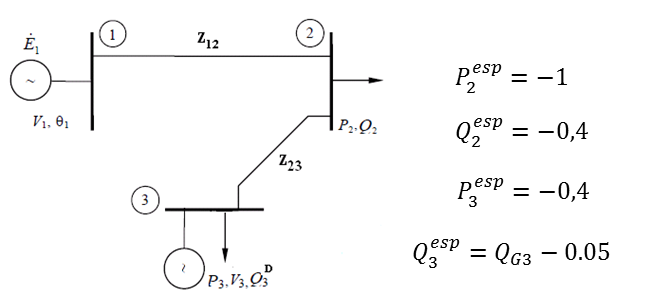
\includegraphics{aula3_10}\protect\caption{\label{fig:aula3_10} Exemplo }
\end{centering}
\end{figure}

\[
P_{1}^{calc}=1,1[1,1(0,33)+V_{2}(-0,33\cos\theta_{2}-3,3\sin\theta_{2})]
\]


\[
Q_{1}^{calc}=1,1[1,1(0,33)+V_{2}(-0,33\sin\theta_{2}-3,3\cos\theta_{2})]
\]


\[
P_{2}^{calc}=V_{2}\cdot[1,1\cdot(-0,33\cdot\cos\theta_{2}+B_{21}\cdot\sin\theta_{2})+V_{2}\cdot(1,706)+1,05\cdot(1,376\cdot\cos\theta_{32}+4,587\cdot\sin\theta_{32})]
\]


\[
Q_{2}^{calc}=V_{2}\cdot[1,1\cdot(1,706\cdot\sin\theta_{2}+7,887\cdot\cos\theta_{2})-V_{2}\cdot(7,887)+1,05\cdot(1,376\cdot\cos\theta_{32}+4,587\cdot\sin\theta_{32})]
\]


\[
P_{3}^{calc}=1,05\cdot[V_{2}\cdot(-1,376\cdot\cos\theta_{32}+4,587\cdot\sin\theta_{32})+1,05\cdot(1,376)]
\]


\[
Q_{3}^{calc}=1,05\cdot[V_{2}\cdot(-1,376\cdot\sin\theta_{32}+4,587\cdot\cos\theta_{32})-1,05\cdot(4,587)]
\]
Considerando:
\[
F(x)={ \begin{matrix} [\triangle { P }_{ 1 } & \triangle { P }_{ 3 } & \triangle { P }_{ 3 } & \triangle { Q }_{ 1 } & \triangle { Q }_{ 2 } & \triangle { Q }_{ 3 }] \end{matrix} }_{ 6 }^{ T }
\]
\[
x={ \begin{matrix} [\theta _{ 1 } & \theta _{ 2 } & \theta _{ 3 } & V_{ 1 } & V_{ 2 } & V_{ 3 }] \end{matrix} }_{ 6 }^{ T }
\]
\[
F(x)={ \begin{matrix} [\triangle { P }_{ 3 } & \triangle { P }_{ 3 } & \triangle { Q }_{ 2 } \end{matrix}] }_{ 3 }^{ T }
\]
\[
x={ \begin{matrix} [\theta _{ 2 } & \theta _{ 3 } & V_{ 2 }] \end{matrix} }_{ 3 }^{ T }
\]
\begin{enumerate}
\item Arbitrar uma condição inicial $(x^{(i)}=x^{(0)})$ e fixar $i=0$;
\[
{ x }^{ (0) }={ \begin{matrix} [0 & 0 & 1 \end{matrix}] }_{ 3 }^{ T }
\]
\item Calcular $F(x^{(i)})$ e verificar a convergência. Se $\max| F(x^{(i)})|\leq \varepsilon$,
parar.
\item Linearizar a função em torno de $(F(x^{(i)}),x^{(i)})$ e igualar
a função a zero para estabelecer o passo $(\varDelta x^{(i)}=x^{(i+1)}-x^{(i)})$
e o novo ponto $(x^{(i+1)})$.
\[
F(x)=F(x^{(i)})+[J(x^{(i)}]\cdot(x^{(i+1)}-x^{(i)})=0
\]
 
\[
x^{(i+1)}=x^{(i)}+[J(x^{(i)}]^{-1}\cdot F(x^{(i)})
\]


Para solucionar o problema proposto devemos determinar a matriz jacobiana:
\begin{figure}[H]
\begin{centering}
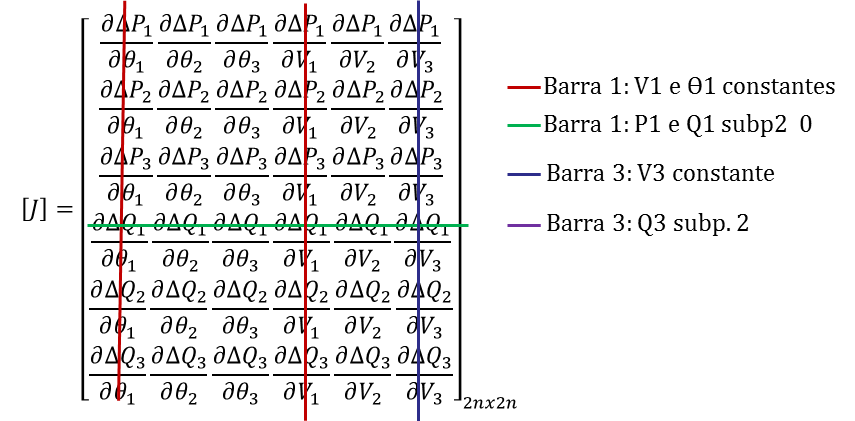
\includegraphics{aula3_11}\protect\caption{\label{fig:aula3_11} Matriz jacobiana do exemplo }
\end{centering}
\end{figure}
O problema apresentado faz com que, para o subproblema 1:
\[
F(x)={ \begin{matrix} [\triangle { P }_{ 3 } & \triangle { P }_{ 3 } & \triangle { Q }_{ 2 } \end{matrix}] }_{ 3 }^{ T }
\]
\[
x={ \begin{matrix} [\theta _{ 2 } & \theta _{ 3 } & V_{ 2 }] \end{matrix} }_{ 3 }^{ T }
\]
Barra 1: $V\theta$(slack bus)

Barra 2: $PQ$(barra de carga)

Barra 3: $PV$(barra de controle de tensão)
\item Fazer $i=i+1$ e voltar ao passo 2.

\end{enumerate}

A matriz Jacobiana par ao problema proposto fica:

\begin{figure}[H]
\begin{centering}
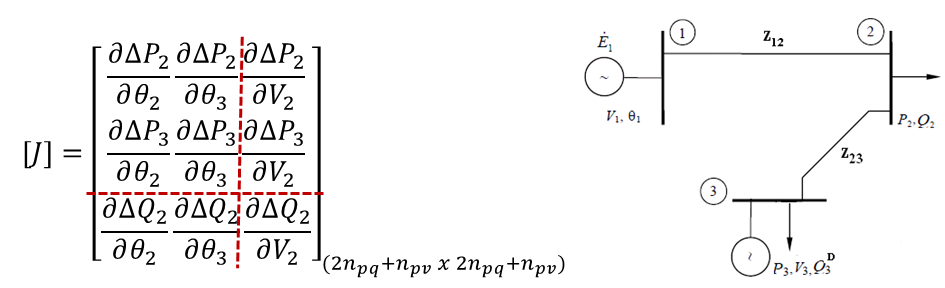
\includegraphics{aula3_12}\protect\caption{\label{fig:aula3_12} Matriz jacobiana }
\end{centering}
\end{figure}
Sendo

$n_{pq}$-Número de barras $PQ$;

$n_{pv}$-Número de barras $PV$;
De outra forma:
\begin{figure}[H]
\begin{centering}
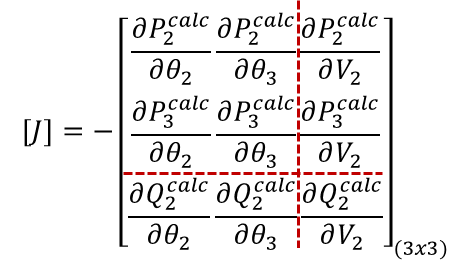
\includegraphics{aula3_13}\protect\caption{\label{fig:aula3_13} Matriz jacobiana }
\end{centering}
\end{figure}

A solução do problema proposto depois de quatro iterações:

\begin{tabular}{|c|c|c|c|c|c|}
\hline 
Barras & V (p.u) & $P_{G}$ & $P_{D}$ & $Q_{G}$ & $Q_{D}$\tabularnewline
\hline 
\hline 
1 (Ref.) ($\theta_{1}=0)$ & 1,1 & - & 0 & - & 0\tabularnewline
\hline 
2 (PQ) & - & 0 & 1 & 0 & 0,4\tabularnewline
\hline 
3 (PQV) & 1,05 & 0,6 & 0,2 & - & 0,05\tabularnewline
\hline 
\end{tabular}
\begin{figure}[H]
\begin{centering}
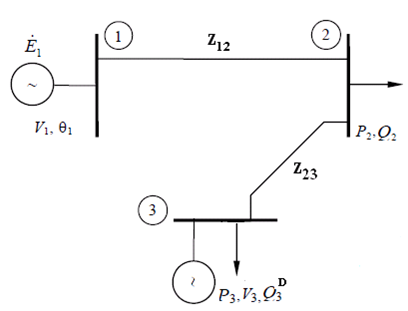
\includegraphics{aula3_14}\protect\caption{\label{fig:aula3_14} Exemplo }
\end{centering}
\end{figure}

$z_{12}=-0,03+0,3j$

$z_{23}=-0,06+0,2j$
\[
{ x }^{ (4) }={ \begin{matrix} { [\theta _{ 2 } }^{ (4) } & { \theta _{ 3 } }^{ (4) } & { V_{ 2 } }^{ (4) }] \end{matrix} }_{ \quad }^{ T }={ \begin{matrix} [-0,1616\quad rad & -0,0958\quad rad & 0,993] \end{matrix} }_{ \quad }^{ T }\quad 
\]
\[
{ x }^{ (4) }={ \begin{matrix} { [\theta _{ 2 } }^{ (4) } & { \theta _{ 3 } }^{ (4) } & { V_{ 2 } }^{ (4) }] \end{matrix} }_{ \quad }^{ T }={ \begin{matrix} [-{ 9,263 }^{ \circ } & { -0,0958 }^{ \circ } & 0,993] \end{matrix} }_{ \quad }^{ T }\quad 
\]

$\varepsilon=0,000001$








%\section{Aula 4}
\label{sec:4}

\subsection{Sistemas Elétricos}
Operar o sistema é definir, a cada etapa do tempo, quais usinas serão acionadas para suprir a demanda de energia elétrica. Além disso os
recursos disponíveis ,por exemplo usinas, possuem capacidades $(G_{i})$ diferentes
e, sobretudo, custos de operação distintos $(c_{i})$. O critério é atender uma demanda $d$ ao menor custo operativo possível garantindo confiabilidade. 

\textbf{Exemplo}

Dois geradores apresentam ofertas de preço e quantidade de geração$(c_{i},G_{i})$ e precisam atender a demanda dos consumidores, que
totaliza $(d)$. No qual o primeiro gerador tem capacidade máxima de produção de $100$ MW e o custo de $100$R\$/MWh enquanto o segundo gerador tem
capacidade máxima de produção de $50$ MW e o custo de $150$R\$/MWh. Esses geradores precisam atender uma demanda de $120$MW (Figura \ref{fig:aula4-1}). Por conveniência, será trabalhado num horizonte de tempo de uma hora, para que potencia
e energia sejam a mesma coisa. e assumindo que a potencia é constante.
\begin{figure}[H]
\begin{centering}
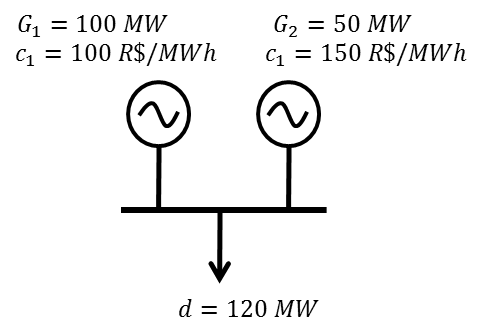
\includegraphics{aula4-1}\protect\caption{\label{fig:aula4-1} Exemplo }
\end{centering}
\end{figure}
Para atender a demanda com esses dois geradores uma possível solução para o problema seria utilizar a potencia do mais barato e depois se necessário utilizar a do mais caro. Essa solução é conhecida como ordem de mérito em custo. Então será necessário utilizar os $100$MW
do primeiro gerador e completar com $20$MW do segundo gerador para assim, atender a demanda (Figura \ref{fig:aula4-2}).
\begin{figure}[H]
\begin{centering}
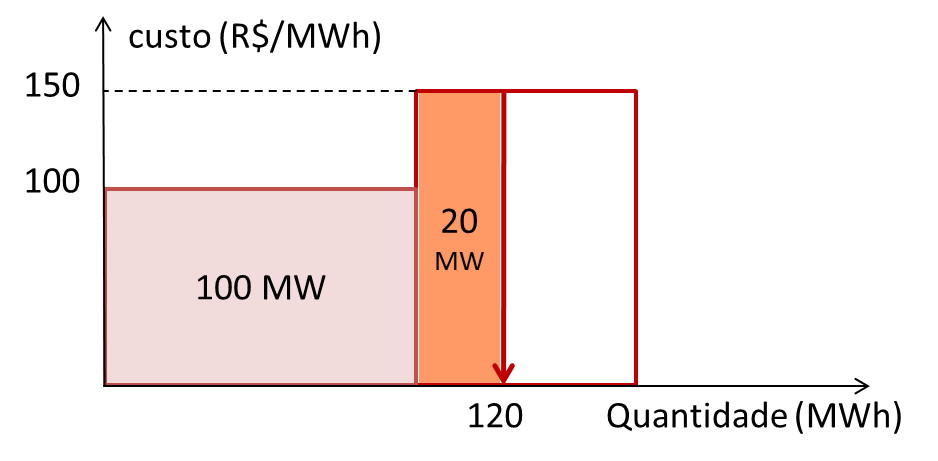
\includegraphics[scale=0.7]{aula4-2}\protect\caption{\label{fig:aula4-2} Despacho por ordem de custo }
\end{centering}
\end{figure}
A modelagem do problema será dado por:
\begin{align}
    & \underset{g\geq0}{\text{Min}} \hspace{1cm} 100g_1+150g_2 \label{eq1} \\
    & \text{s.a}  \hspace{2.2cm} g_1+g_2 \geq 120; \label{eq2} \\
    &             \hspace{2.65cm} g_1\leq 100, \label{eq3}\\
    &             \hspace{2.65cm} g_2\leq 50. \label{eq4}
\end{align}

Assim, a visualização gráfica com a área viável é apresentado na figura \ref{fig:aula4-3}.
\begin{figure}[H]
\begin{centering}
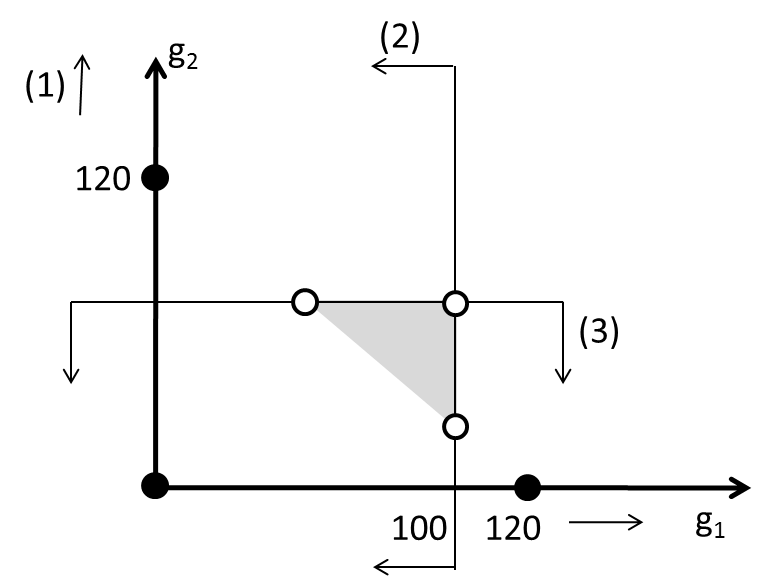
\includegraphics[scale=0.7]{aula4-3}\protect\caption{\label{fig:aula4-3} Gráfico exemplo }
\end{centering}
\end{figure}
Adicionando o gradiente e verificando a solução ótima do problema:

\begin{figure}[H]
\begin{centering}
\includegraphics[scale=0.70]{aula4-4}\protect\caption{\label{fig:aula4-4} Gráfico exemplo gradiente }
\end{centering}
\end{figure}

\begin{figure}[H]
\begin{centering}
\includegraphics[scale=0.8]{aula4-5}\protect\caption{\label{fig:aula4-5} Gráfico exemplo igualdade}
\end{centering}
\end{figure}

Através da figura (\ref{fig:aula4-5}), é possível concluir que a restrição (\ref{eq2}) será alterada, conforme apresentado:
\begin{align}
    & \underset{g\geq0}{\text{Min}} \hspace{1cm} 100g_1+150g_2 \label{eq5} \\
    & \text{s.a}  \hspace{2.2cm} g_1+g_2 = 120; \label{eq6} \\
    &             \hspace{2.65cm} g_1\leq 100, \label{eq7}\\
    &             \hspace{2.65cm} g_2\leq 50. \label{eq8}
\end{align}
A primeira restrição(\ref{eq6}) é o objetivo primário por ser necessário atender a demanda independente do custo gerado, e posteriormente será avaliado o menor custo de geração. Se por exemplo o nosso objetivo primário fosse atender o custo, a melhor solução para o problema é não produzir. Assim,primeiramente precisamos  atender as restrições para depois avaliar o objetivo, no caso menor custo.
Então o problema de despacho pode ser modelado da seguinte maneira,
\begin{align}
    & \underset{g\geq0}{\text{Min}} \hspace{1cm} \sum_{i=1}^{n}c_{i}\cdot g_{i} \label{eq9} \\
    & \text{s.a}  \hspace{2.2cm} \sum_{i=1}^{n}g_{i}\geq d; \label{eq10} \\
    &             \hspace{2.65cm}g_{i}\leq G_{i} \forall i=1,...,n. \label{eq11}
\end{align}

O objetivo é minimiza a soma dos custos variáveis referente a sua geração (equação \ref{eq9}) , sendo que precisamos atender a demanda (equação \ref{eq10}) e atendendo o máximo de geração de cada usina (equação \ref{eq11}).
Supondo que a demanda precise de um MWH a mais do problema modelado anteriormente,qual o custo desse MWH a ser atendido?
O objetivo descobrir o custo adicional do próximo MWH é interessante
para saber quanto cobrar a mais no caso de entrar uma MWH no modelo.
O conceito de usina marginal ou unidade marginal é a usina que está na
margem das usinas que estão produzindo, ou seja, o ultimo gerador
produzindo.Assim, é formado o custo marginal do sistema.

O custo pode ser representado por,
\[
\Delta C^{*}(d)=C^{*}(d+1)-C^{*}(d).
\]

Temos que,

\[
\frac{\partial C^{*}(d)}{\partial d}=\lim_{\Delta\rightarrow0^{+}}\frac{C^{*}(d+\Delta-C^{*}(d))}{\Delta} ,
\]


\[
\frac{\partial C^{*}(d)}{\partial d}=c_{i^{*}},
\]
$i^{*}$é o gerador marginal.
Como no exemplo apenas o gerador 2 possui potencia para atender o
próximo MWH, então seu custo adicional será o custo $c_{2}$ ,\[
\Delta C^{*}(d)=[C^{*}(d)+c_{2}\cdot1]-C^{*}(d)=c_{2},
\]
 e pode ser representado na figura abaixo:

\begin{figure}[H]
\begin{centering}
\includegraphics[scale=0.8]{aula4-6}\protect\caption{\label{fig:aula4-6} Derivada nos pontos}
\end{centering}
\end{figure}
Então aplicado ao exemplo anterior será dado por:
\begin{figure}[H]
\begin{centering}
\includegraphics[scale=0.8]{aula4-7}\protect\caption{\label{fig:aula4-7} Gráfico exemplo com custo adicional}
\end{centering}
\end{figure}
A função custo será dada pela figura (\ref{fig:aula4-8}) e possui propriedades importantes:
\begin{enumerate}
\item é linear por partes;
\item tem primeira derivada descontínua;
\item é crescente;
\item é convexa;
\end{enumerate}
\begin{figure}[H]
\begin{centering}
\includegraphics[scale=0.8]{aula4-8}\protect\caption{\label{fig:aula4-8} Função custo}
\end{centering}
\end{figure}
\subsection{Teoria da dualidade}
\begin{enumerate}
\begin{itemize}
\item Como funciona o processo de “dualização” de restrições (relaxação langrangeana)?
\begin{equation*}
\begin{aligned}
& z_{p}^{*}=\underset{x\geq0}{\text{Max}}
& & c^{T}x \\
& \text{s.a}
& & Ax \leq b.
\end{aligned}
\end{equation*}
\item O processo de ``dualização'' implica em relaxar alguma das restrições
(ou todas) do problema prima e incorporar uma penalização na função
objetivo sobre a viabilidade das soluções.
\begin{equation*}
\begin{aligned}
& z_{p}^{*}\leq \theta(y)=\underset{x\geq0}{\text{Max}}
& & c^{T}x+y^{T}(b-Ax)  \forall  y\geq 0 \\
& \text{s.a}
& & Ax \leq b.
\end{aligned}
\end{equation*}
\[
z_{p}^{*}\leq\theta(y)\leq\phi(y)=\max_{x\geq0}c^{T}\cdot x+y^{T}\cdot(b-A\cdot x)\forall y\geq0
\]
Uma interpretação para a variável dual($y^{T}(b-A\cdot x)$) no exemplo dado na aula 1: O dono da fábrica agora pode vender ou comprar a sobra ou déficit de insumos em “um mercado” (ilimitado) por preço y.
\item Como se comporta a função dual lagrangeana?

\[
z_{p}^{*}\leq\phi(y)=\max_{x\geq0}c^{T}\cdot x+y^{T}\cdot(b-A\cdot x)\forall y\geq0
\]
\item Dado um vetor $y$ de multiplicadores de Lagrange,
\[
z\leq\phi(y)=\max_{x\geq0}(c^{T}-y^{T}\cdot A)\cdot x+y^{T}\cdot b=\left\{ \begin{array}{c}
y^{T}\cdot b,sec^{T}-y^{T}\cdot A\leq0\\
+\infty,casocontr\acute{a}rio
\end{array}\right\} 
\]
\item O processo de relação lagrangeana busca uma vetor y que minimize $\phi(y)$. Logo, o segundo caso (que proporciona valor infinito) será sempre evitado.A interpretação para esse comportamento é:
\item[-] Se o lucro unitário de produção $(c^{T})$ for inferior à receita de venda de seus insumos $(y^{T}A)$ no mercado ao preço $y$ , então paramos a produção e vendemos todos os insumos no mercado, resultando em um lucro de $y^{T}b$.
\item[-] Caso contrário, ocorre a possibilidade de arbitragem, onde podemos comprar no mercado os insumos por preços que geram um custo inferior ao lucro de produção. Assim, compramos infinito e vendemos infinito, obtendo assim resultado ilimitado.
\item O problema dual busca um vetor y que minimize $\phi(y)$.Logo, o segundo caso será sempre evitado.
$$
z\leq\min_{y\geq0}\phi(y)=\min_{y\geq0}\left\{ \begin{array}{c}
y^{T}\cdot b,sec^{T}-y^{T}\cdot A\leq0\\
+\infty,casocontr\acute{a}rio
\end{array}\right\} =\begin{array}{cc}
\min_{y\geq0} & y^{T}\cdot b\\
s.a: & y^{T}\cdot A\geq c^{T}
\end{array}
$$
Assim, Quais são os preços y's que minimizam essa função. A busca pelos preços de mercado que deixa o produtor indiferente entre produzir e vender os insumos nos mercados.
\item Assim, temos o seguinte par primal-dual:
$$
z_{p}^{*}=\begin{array}{cc}
\max_{x\geq0} & c^{T}\cdot x\\
s.a: & A\cdot x\leq b
\end{array}\leq z_{d}^{*}=\begin{array}{cc}
\min_{y\geq0} & y^{T}\cdot b\\
s.a: & y^{T}\cdot A\geq c^{T}
\end{array}
$$
\item O teorema da dualidade fraca diz que (Primal de Maximização):
\item[-]  O valor mínimo do problema Dual ( de minimização) é superior ao máximo do problema primal (maximização).
\item[-] Isso torna-se óbvio depois de mostrado o processo de construção do
dual da maneira que apresentamos aqui. Este foi concebido para sempre
gerar um limite superior para o problema primal.
\item O teorema da dualidade Forte diz que ( Primal de Maximização):
\item[-] No ótimo o valor da função objetivo de qualquer par primal-dual decorrente de um problema de programação linear é sempre o mesmo!
$$
z_{p}^{*}=\begin{array}{cc}
\max_{x\geq0} & c^{T}\cdot x\\
s.a: & A\cdot x\leq b
\end{array} = z_{d}^{*}=\begin{array}{cc}
\min_{y\geq0} & y^{T}\cdot b\\
s.a: & y^{T}\cdot A\geq c^{T}
\end{array}
$$
\begin{figure}[H]
\begin{centering}
\includegraphics[scale=0.8]{aula4-9}\protect\caption{\label{fig:aula4-9} GAP dual}
\end{centering}
\end{figure}
\item Talvez a mais importante, ou pelo menos mais conhecida e difundida
em diversas áreas, devido à relação entre o problema primal e o dual
seja a interpretação da variável dual como ``preço sombra'' ou custo
marginal dos recursos:
\item[-] Em problemas convexos, em que vale a dualidade forte, a variável dual pode ser interpretada como a derivada parcial do valor ótimo da função
objetivo do primal, com relação ao lado direito da restrição associada
a esta variável.
\item[-] Que em ultima análise é o multiplicador de lagrange
\[
z_{p}^{*}=z_{d}^{*}=y^{*T}\cdot b
\]


\[
\frac{\partial z_{p}^{*}}{\partial b}=\left[\frac{\partial z_{p}^{*}}{\partial b_{1}},...,\frac{\partial z_{p}^{*}}{\partial b_{m}}\right]=\left[y_{1}^{*},...,y_{m}^{*}\right]=y^{*T}.
\]

\end{itemize}
\end{enumerate}
\textbf{Exemplo: despacho centralizado vs. competição perfeita}

O despacho ótimo ``centralizado'' de um período, que visa atender
uma demanda $d$ (MWh) utilizando os recursos disponíveis (capacidade
$G_{i}$) é dado pelo seguinte problema:
\begin{align}
    & \underset{g\geq0}{\text{Min}} \hspace{1cm} \sum_{i=1}^{n}c_{i}\cdot g_{i} \label{eq12} \\
    & \text{s.a}  \hspace{2.2cm} \sum_{i=1}^{n}g_{i}\geq d; \label{eq13} \\
    &             \hspace{2.65cm}g_{i}\leq G_{i} \forall i=1,...,n. \label{eq14}
\end{align}

Para que este problema atinja o seu objetivo, é importante que os
agentes informe os seus reais custo operativos e capacidades ($c_{i},G_{i}$).
Um processo iterativo (competição) que controla o preço de mercado
da energia, onde os geradores (price-takers) ofertam preço (custos reais) e quantidade (capacidades máximas), visando maximizar os seus lucros individualmente com a venda de energia através de um leilão de preço uniforme, proporciona o mesmo despacho (solução de geração) que o despacho de
mínimo custo.
Assim, começamos por dualização a restrição de atendimento à demanda. Onde, para todo $\pi\geq0$ teremos a seguinte relação:
\[
C^{*}\geq C_{d}^{*}(\pi)=Min_{g\geq0}\sum_{i=1}^{n}c_{i}\cdot g_{i}+\pi\cdot\left(d-\sum_{i=1}^{n}g_{i}\right)
\]

\[
s.a \, g_{i}\leq G_{i}\forall i=1, ... ,n.
\]
Em seguida, rearranjamos os termos de maneira a colocar o $g_{i}$ em evidência:


\[
C^{*}\geq C_{d}^{*}(\pi)=Min_{g\geq0}\pi\cdot d-\sum_{i=1}^{n}(\pi-c_{i})\cdot g_{i}
\]


\[
s.a \, g_{i}\leq G_{i}\forall i=1,...,n.
\]


Como o primeiro termo não depende da decisão $g$, este pode ser colocado fora do  $min$ e podemos verificar que o $min$ de uma função negativa é o $max$ desta função colocando o sinal de negativo para fora da função $max$. Temos que ,
\[
C^{*}\geq C_{d}^{*}(\pi)=\pi\cdot d-\sum_{i=1}^{n}Max_{g\geq0_{i}}(\pi-c_{i})\cdot g_{i}
\]


\[
s.a \, g_{i}\leq G_{i}\forall i=1,...,n.
\]
Por fim, repare que o problema de minimização pode ser decomposto
em $n$ problemas, em que cada um pode ser substituído por um de maximização.

Assim, dado o preço do mercado $\pi$ é encontrado o problema de maximização da receita líquida de venda ($Max_{g\geq0_{i}}(\pi-c_{i})\cdot g_{i}$).
O problema resultante é o problema em que cada agente gerador visa maximizar a sua renda vendendo energia a um preço $\pi$(R\$/MWh) e a demanda (inelástica) paga o mesmo preço pela aquisição dessa energia.
Onde,
\[
C^{*}\geq Max_{\pi\geq0}\pi\cdot d-\sum_{i=1}^{n}R_{i}^{*}(\pi)
\]


\[
R_{i}^{*}(\pi)=Max_{g_{i}\geq0}(\pi-c_{i})\cdot g_{i}
\]


\[
s.a \, g_{i}\leq G_{i}\forall i=1,...,n.
\]

\begin{figure}[H]
\begin{centering}
\includegraphics[scale=0.8]{aula4-10}\protect\caption{\label{fig:aula4-10} Operação centralizada vs competitiva}
\end{centering}
\end{figure}
E se a capacidade de geração não for suficiente para suprir a demanda?
\begin{figure}[H]
\begin{centering}
\includegraphics[scale=0.5]{aula4-11}\protect\caption{\label{fig:aula4-11} Gráfico com o aumento da demanda}
\end{centering}
\end{figure}
Corte de carga (déficit)

Se a demanda for maior que a soma das capacidades máximas, então o
problema é inviável. Porém,na prática o problema não é inviável, mas uma fração da demanda não será suprida: ``corte de carga'' ou déficit (diferente de racionamento).Na realidade o sistema é operado cortando algumas cargas (diminuindo as cargas) por exemplo uma área da distribuidora ,desliga algum consumidor,desligamentos seletivos, etc.
\begin{figure}[H]
\begin{centering}
\includegraphics[scale=0.7]{aula4-12}\protect\caption{\label{fig:aula4-12} Viabilidade do proble,a }
\end{centering}
\end{figure}
Caso falte capacidade de produção, sera necessário transformar um restrição hard (inicialmente a restrição de atender à demanda) para um restrição suavizada (atender a demanda sempre que possível) então será necessário diminuir a demanda assim, esse corte de carga é ótimo. 
Para isso introduzimos uma variável ao problema que age como se
fosse um gerador, porem é um corte de carga.Essa variável adicionada ao problema  é uma variável de decisão e é penalizada no problema na função objetivo com um custo de deficit maior que o custo dos outros geradores.
Assim é possível construir a curva de déficit, com diferente patamares
que será modelado na seguinte maneira:
\begin{align}
    & \underset{g\geq0, r\geq0}{\text{Min}} \hspace{1cm} \sum_{i=1}^{n}c_{i}\cdot g_{i} + c_{d}\cdot r \label{eq15} \\
    & \text{s.a}  \hspace{2.2cm} \sum_{i=1}^{n}g_{i} + r\geq d \label{eq16} \\
    &             \hspace{2.65cm}g_{i}\leq G_{i} \forall i=1,...,n.\label{eq17}
\end{align}

Essa função é conhecida como custo de déficit. E será representada,

\begin{align}
    & \underset{g\geq0, r\geq0}{\text{Min}} \hspace{1cm} \sum_{i=1}^{n}c_{i}\cdot g_{i} + \sum_{j=1}^{m}c_{j}^{d}\cdot r_{j} \label{eq16} \\
    & \text{s.a}  \hspace{2.2cm} \sum_{i=1}^{n}g_{i} + \sum_{j=1}^{m}r_{j}\geq d \label{eq17} \\
    &             \hspace{2.65cm}g_{i}\leq G_{i} \forall i=1,...,n\label{eq18}\\
    &                \hspace{2.65cm}r_{j}\leq \bar{r}_{j} \forall j=1,...,m.\label{eq19}
\end{align}
A figura (\ref{fig:aula4-14}) representa a adição do custo de déficit no modelo.
\begin{figure}[H]
\begin{centering}
\includegraphics[scale=0.8]{aula4-14}\protect\caption{\label{fig:aula4-14} Função custo com o custo de déficit }
\end{centering}
\end{figure}

A figura (\ref{fig:aula4-15}) é conhecida como curva de duração de demanda, no eixo ($x$) está representada a frequência no ano e o eixo($y$) representa a demanda. Uma interpretação para este gráfico é que quando a demanda atingir uma carga crítica de ($5\%$) com uma duração de ($5\%$) do ano, estaríamos utilizando geradores flexíveis, geradores de base e geradores inflexível. 
Geradores de bases praticamente inflexível (exemplo:nuclear e carvão) produzem energia ($100\%$) durante o ano e possuem custo de investimento caro e custo de operação barato ou seja, são os primeiro a serem ligados.Geradores de bases flexíveis conseguem gerar e desligar se necessário com um taxa de desligamento (não acionamento), as vezes a demanda fica menor do que o custo variável destes. Geradores flexíveis  são responsáveis por atender demandas no intervalo acima, o os demais geradores são conhecidos como geradores de pico que vivem para atender aproximadamente 3\% da carga. Só em eventos raros ele será acionado para produzir. Porem,qual deve ser o valor que se paga para os geradores de pico para produzir sabendo que eles vão produzir em poucas horas.
\begin{figure}[H]
\begin{centering}
\includegraphics[scale=0.7]{aula4-15}\protect\caption{\label{fig:aula4-15}  Curva de duração de demanda}
\end{centering}
\end{figure}

\subsection{Restrições de rede}
\textbf{Exemplo}

Sejam dois geradores em locais diferentes ligados por uma linhas de transmissão onde, os geradores possuem capacidades finitas e limites de transmissão. O gerador $1$ tem capacidade máxima de produção de $100$ MW e o custo de $100$R\$/MWh enquanto o  gerador $2$  tem capacidade máxima de produção de $50$ MW e o custo de $150$R\$/MWh.Esses geradores precisam atender uma demanda de $120$MW (Figura \ref{fig:aula4-16}). O diferencial deste exemplo para o exemplo apresentando anteriormente está na linha de transmissão. O gerador $1$ pode transmitir $80$ MW e a linha de transmissão do gerador $2$ pode passar $80$MW para atender a demanda de $120$MW.
\begin{figure}[H]
\begin{centering}
\includegraphics[scale=0.8]{aula4-16}\protect\caption{\label{fig:aula4-16} Exemplo ligado por linha de transmissão}
\end{centering}
\end{figure}
O despacho ótimo encontrado no primeiro exemplo de $g_{1}^{*}=100$ não pode ser injetado na rede, então neste caso essa solução será inviável.
A seta na (Figura \ref{fig:aula4-16}) representa o sentido do fluxo e por convenção adotaremos que quando a senta sai do gerador perde energia então temos fluxo negativo e quando entra o gerador recebe energia e assim o fluxo é positivo.

O modelo de transporte, possui esse nome por não considerar algumas características elétricas do na rede, será dado por:
\begin{itemize}
\item Restrição de atendimento à demanda (balanço de potência ou nodal)
por barra:

\[
g_{1}-f_{1}-f_{2}=0
\]


\[
g_{2}+f_{2}-f_{3}=0
\]


\[
f_{1}+f_{3}=d
\]
\item O sinal do fluxo depende da convenção: (+) se passa no sentido das setas e (-) caso contrário.
\item Então, a restrição de capacidade das linhas é:

\[
-F_{l}\leq f_{1}\leq F_{l}
\]
\item Matriz de incidência de fluxo em redes: $+1$ se a aresta $l$ chega
no vértice $i$ e $-1$ se sai:
\[
\begin{array}{ccccccc}
g_{1} &  & -f_{1} & -f_{2} &  & = & 0\\
 & g_{2} &  & +f_{2} & -f_{3} & = & 0\\
 &  & f_{1} &  & +f_{3} & = & d
\end{array}
\]
Ou seja, tudo que entra na barra é igual a tudo que sai dessa barra.
\end{itemize}
Assim, podemos montar o modelo de transporte completo do exemplo dado por:
\[
\min_{g_{i}\geq0,f_{l}}100g_{1}+150g_{2}
\]
\[
\begin{array}{ccccccc}
s.a:\\
g_{1} &  & -f_{1} & -f_{2} &  & = & 0\\
 & g_{2} &  & +f_{2} & -f_{3} & = & 0\\
 &  & f_{1} &  & +f_{3} & = & d\\
-60 & \leq & f_{1} &  &  & \leq & 60\\
-20 & \leq &  & f_{2} &  & \leq & 20\\
-80 & \leq &  &  & f_{3} & \leq & 80\\
g_{1} &  &  &  &  & \leq & 100\\
 & g_{2} &  &  &  & \leq & 50.
\end{array}
\]
\begin{figure}[H]
\begin{centering}
\includegraphics[scale=0.7]{aula4-17}\protect\caption{\label{fig:aula4-17} Solução ótima do exemplo}
\end{centering}
\end{figure}

A Figura (\ref{fig:aula4-17} ) representa a solução ótima do problema.

\textbf{O custo marginal nodal}
O custo de atender $1$ MWh a mais, sendo que neste exemplo podemos adicionar esse MWh para cada barra do sistema.
No caso da barra $1$, o custo adicional de operação ótima para suprir $1$ MWh será representado na figura (\ref{fig:aula4-18} ) e  modelado da seguinte maneira:
\[
\min_{g_{i}\geq0,f_{l}}100g_{1}+150g_{2}
\]
\[
\begin{array}{ccccccc}
s.a:\\
g_{1} &  & -f_{1} & -f_{2} &  & = & +1\\
 & g_{2} &  & +f_{2} & -f_{3} & = & 0\\
 &  & f_{1} &  & +f_{3} & = & d\\
-60 & \leq & f_{1} &  &  & \leq & 60\\
-20 & \leq &  & f_{2} &  & \leq & 20\\
-80 & \leq &  &  & f_{3} & \leq & 80\\
g_{1} &  &  &  &  & \leq & 100\\
 & g_{2} &  &  &  & \leq & 50.
\end{array}
\]

\begin{figure}[H]
\begin{centering}
\includegraphics[scale=0.7]{aula4-18}\protect\caption{\label{fig:aula4-18} Aumento da demanda na barra 1 }
\end{centering}
\end{figure}
O custo adicional de operação encontrada é de $\pi_{1}=100$ R$\$$/MWh representado na figura (\ref{fig:aula4-19} ).
\begin{figure}[H]
\begin{centering}
\includegraphics[scale=0.7]{aula4-19}\protect\caption{\label{fig:aula4-19} Custo adicional na barra 1 }
\end{centering}
\end{figure}

A barra $2$, o custo adicional de operação ótima para suprir $1$ MWh será representado na figura (\ref{fig:aula4-20} ) e a modelagem dada por:
\[
\min_{g_{i}\geq0,f_{l}}100g_{1}+150g_{2}
\]
\[
\begin{array}{ccccccc}
s.a:\\
g_{1} &  & -f_{1} & -f_{2} &  & = & 0\\
 & g_{2} &  & +f_{2} & -f_{3} & = & +1\\
 &  & f_{1} &  & +f_{3} & = & d\\
-60 & \leq & f_{1} &  &  & \leq & 60\\
-20 & \leq &  & f_{2} &  & \leq & 20\\
-80 & \leq &  &  & f_{3} & \leq & 80\\
g_{1} &  &  &  &  & \leq & 100\\
 & g_{2} &  &  &  & \leq & 50.
\end{array}
\]

\begin{figure}[H]
\begin{centering}
\includegraphics[scale=0.7]{aula4-20}\protect\caption{\label{fig:aula4-20} Custo adicional na barra 2}
\end{centering}
\end{figure}

Então,o custo adicional de operação encontrada é de  $\pi_{2}=150$ R$\$$/MWh.
Ao adicionar $1$ MWh na demanda, a barra $2$ irá atender essa demanda extra sem necessidade de cortar carga, conforme apresentado na figura (\ref{fig:aula4-21}).
\[
\min_{g_{i}\geq0,f_{l}}100g_{1}+150g_{2}
\]
\[
\begin{array}{ccccccc}
s.a:\\
g_{1} &  & -f_{1} & -f_{2} &  & = & 0\\
 & g_{2} &  & +f_{2} & -f_{3} & = & 0\\
 &  & f_{1} &  & +f_{3} & = & d+1\\
-60 & \leq & f_{1} &  &  & \leq & 60\\
-20 & \leq &  & f_{2} &  & \leq & 20\\
-80 & \leq &  &  & f_{3} & \leq & 80\\
g_{1} &  &  &  &  & \leq & 100\\
 & g_{2} &  &  &  & \leq & 50.
\end{array}
\]

\begin{figure}[H]
\begin{centering}
\includegraphics[scale=0.8]{aula4-21}\protect\caption{\label{fig:aula4-21} Custo adicional na demanda}
\end{centering}
\end{figure}

De maneira geral podemos associar os  $\pi_{i}$ que são as variáveis duais destas restrições do ponto ótimo do dual, da seguinte forma:
\[
\min_{g_{i}\geq0,f_{l}}100g_{1}+150g_{2}
\]
\[
\begin{array}{ccccccc}
s.a:\\
g_{1} &  & -f_{1} & -f_{2} &  & = & 0 (\pi_{1}) \\
 & g_{2} &  & +f_{2} & -f_{3} & = & 0 (\pi_{2})\\
 &  & f_{1} &  & +f_{3} & = & d (\pi_{3})\\
-60 & \leq & f_{1} &  &  & \leq & 60\\
-20 & \leq &  & f_{2} &  & \leq & 20\\
-80 & \leq &  &  & f_{3} & \leq & 80\\
g_{1} &  &  &  &  & \leq & 100\\
 & g_{2} &  &  &  & \leq & 50.
\end{array}
\]

Modelo DC linearizado

Este modelo adicionar mais uma restrição ao problema,sendo esta uma restrição linearizada do fluxo de potência visto na aula 3.
Para isso devemos incorporar a segunda lei de Kirchhoff:
\[
f_{l}=\frac{1}{x_{l}}(\theta_{ori(l)}-\theta_{des(l)}),
\]
o fluxo numa linha($f_{l}$) é proporcional ao inverso da reatância(${x_{l}$) e a diferença de ângulos entra as barras ($\theta_{ori(l)}-\theta_{des(l)}$). 
Supondo $x_{l}=1$:
$$f_{1}=\theta_{1}-\theta_{3}$$
$$f_{2}=\theta_{1}-\theta_{2}$$
$$f_{3}=\theta_{2}-\theta_{3}$$

Assim, temos uma restrição por ciclo:
$$f_{1}=\theta_{1}-\theta_{3}$$
$$f_{2}=\theta_{1}-\theta_{2}$$
$$f_{3}=\theta_{2}-\theta_{3}.$$

Criando assim uma dependência linear dos fluxos. Logo, $f_{1}-f_{2}=f_{3}$ ou $f_{2}=f_{1}-f_{3}$.
Devido a restrição acima e ao limite do fluxo na linha 2,temos: $-20\leq f_{1}-f_{3}\leq20$.

O despacho ótimo sem rede é inviável mesmo que exista capacidade suficiente
de transmissão.
Agora, supondo que amplie a capacidade de $f_{1}$ e pela dependência não
é viável este problema pelo fato de, $100-20=80$, que não atende a restrição de $-20\leq f_{1}-f_{3}\leq20$ (Figura \ref{fig:aula4-22}).

\begin{figure}[H]
\begin{centering}
\includegraphics[scale=0.6]{aula4-22}\protect\caption{\label{fig:aula4-22} Problema inviável }
\end{centering}
\end{figure}

\subsection{Confiabilidade}
\begin{itemize}
\item Frequentes apagões demonstram que a confiabilidade do sistema ainda é um tema não resolvido, cortes de carga culminando em ações terríveis.
\item Os níveis de reserva (baixos) colocam o sistema em risco mesmo sob
contingências corriqueiras
\begin{figure}[H]
\begin{centering}
\includegraphics[scale=0.8]{aula4-23}\protect\caption{\label{fig:aula4-23} Apagões}
\end{centering}
\end{figure}
\item Falhas em cascata são uma das principais causas de grandes apagões
\item As redes elétricas são frequentes alvos de ataques
\begin{figure}[H]
\begin{centering}
\includegraphics[scale=0.8]{aula4-24}\protect\caption{\label{fig:aula4-24} Falhas em cascata e ataques a redes elétricas }
\end{centering}
\end{figure}
\end{itemize}
Então é necessário garantir o suprimento da demanda com algum critério de "confiança", uma possibilidade para isso é associar a probabilidade à confiabilidade, conforme apresentado a seguir:

$$Prob(Demanda \, n\tilde{a}o \, suprida>0)\leq3\%$$,
ou seja, corte de carga ser positivo e limitado
.
Se a probabilidade de um dos geradores falhar é $5\%$ e as falhas
são independentes:

$P(Falhar\,G1)=P(Falha\,rG2)=5\%$

$P(Falhar\,G1\,e\,G2)=0,25\%$

Dado que os dois geradores são necessários para suprir a demanda.Logo, basta garantir que o sistema tenha reserva suficiente para suprir a demanda mesmo que um gerador falhe. Este é o critério $n-1$ de segurança. O sistema tem que atender a carga mesmo que um sistema da rede falhe.

Serviços ancillares são principais reservas girantes (capacidade ociosa nos geradores acoplados que permitem o sistema retomar o equilíbrio ,frequência e tensão, através do ``redespacho'' dos geradores remanescentes).

O modelo de despacho econômico de potência e reservas (Figura \ref{fig:aula4-25} tem como objetivo alocar as reservas de maneira que elas sejam entregaveis e garantem a entregabilidade das reservas mesmo que um gerador falhe. 

\begin{figure}[H]
\begin{centering}
\includegraphics[scale=0.5]{aula4-25}\protect\caption{\label{fig:aula4-25} Modelo de despacho econômico de potência e reservas }
\end{centering}
\end{figure}

Programação pré-contingência ou programação nominal é a programação caso nada acontece ou seja,geração maior que a demanda, geração mais a reserva dentro da capacidade,geração mais a potencia de reserva com uma reserva máxima
da capacidade.

Caso ocorra falha do gerador $1$: redespacho inviável do gerador $2$ dentro da reserva programada de $50$ MW para atender a carga de $100$ Mw (Figura \ref{fig:aula4-26}).
\begin{figure}[H]
\begin{centering}
\includegraphics[scale=0.5]{aula4-26}\protect\caption{\label{fig:aula4-26} Falha do gerador 1}
\end{centering}
\end{figure}
Na figura \ref{fig:aula4-27} redespacho viável dentro das reservas programadas para atender a carga de $100$ Mw em qualquer estado pós-contingência. 

\begin{figure}[H]
\begin{centering}
\includegraphics[scale=0.5]{aula4-27}\protect\caption{\label{fig:aula4-27} Falhar qualquer estado pós-contingência }
\end{centering}
\end{figure}

O despacho de potência e reservas apresentado de maneira geral pode ser expresso da seguinte maneira:
\begin{itemize}
\item Critério de confiabilidade n-K
\item Despacho de potência e reserva para o estado pré-contingência que garanta um redespacho viável mesmo que K elementos falhem
\item Garantir a entregabilidade das reservas
\item Considerando falaha de geradores e linhas de transmissão
\item Falha determinada pelo vetor de disponibilidade: vale 1 se o elemento está disponível e zero caso contrário.
\item $$a(k)=\left[a^{G}(k)|a^{L}(k)\right]\in\{0,1\}^{n}$$
\item $$\sum_{i\in U}a_{i}^{G}(k)+\sum_{l\in L}a_{l}^{L}(k)\geq n-K$$
\end{itemize}
Assim temos a modelagem completa :
\begin{figure}[H]
\begin{centering}
\includegraphics[scale=0.5]{aula4-28}\protect\caption{\label{fig:aula4-28} Problema completo}
\end{centering}
\end{figure}
Considerando todo cenário de demanda líquida:
\begin{figure}[H]
\begin{centering}
\includegraphics[scale=0.5]{aula4-29}\protect\caption{\label{fig:aula4-29} Problema completo considerando todo cenário de demanda líquida}
\end{centering}
\end{figure}

\textbf{Preço da energia com segurança}
\begin{itemize}
\item O preço da energia está associado ao incremento de custo devido a
um incremento na demada dado por:

\[
\pi_{b}=\pi_{b}^{pre}+\sum_{k\in C}\pi_{bk}^{pos}\forall b\in B
\]
Onde $\pi_{b}^{pre}$ e $\pi_{bk}^{pos}$ são as variáveis duais das
restrições abaixo:

\[
\sum_{i\in U_{b}}g_{i}+\sum_{l\in L_{b}^{+}}f_{l}-\sum_{l\in L_{b}^{-}}f_{l}=d_{b}(\pi_{b}^{pre})\forall b\in B
\]


\[
\sum_{i\in U_{b}}g_{i}^{(k)}+\sum_{l\in L_{b}^{+}}f_{l}^{(k)}-\sum_{l\in L_{b}^{-}}f_{l}^{(k)}=d_{b}(\pi_{b}^{pos})\forall b\in B,k\in C
\]

\end{itemize}

\subsection{Unit Commitment}
\begin{itemize}
\item $v_{it}\in\{0,1\}$: vale $1$ se o gerador $i$ estiver ligado em $t$
\item Adicionar o custo de start-up e shutdown $C^{on}x_{it}^{on}+C^{off}x_{it}^{off}$
\item \[
v_{it}-v_{it-1}=x_{it}^{on}-x_{it}^{off}=1-0
\]


Restrições de rampa:

\[
-\Delta_{i}^{dn}\leq g_{it+1}-g_{it}\leq\Delta_{i}^{up}
\]
\begin{figure}[H]
\begin{centering}
\includegraphics[scale=0.5]{aula4-30}\protect\caption{\label{fig:aula4-30} }
\end{centering}
\end{figure}

\item \[
v_{it}-v_{it-1}=x_{it}^{on}-x_{it}^{off}=0-1
\]


\begin{figure}[H]
\begin{centering}
\includegraphics[scale=0.5]{aula4-31}\protect\caption{\label{fig:aula4-31} }
\end{centering}
\end{figure}
\end{itemize}
\subsection{Operacionalização}

Planejamento para o dia seguinte

\begin{itemize}
\item Modelos de unit commitment: custo varáveis e fixos de partida, desligamento,restrições de tecnologias, restrições de rede e confiabilidade (segurança).
\item Definir quais centrais estarão ligadas, em quais horas e suas quantidades de produção nominal e reservas.
\item Incertezas: demanda, geração renovável, disponibilidade de equipamentos
\end{itemize}

\begin{figure}[H]
\begin{centering}
\includegraphics[scale=0.5]{aula4-32}\protect\caption{\label{fig:aula4-32} Planejamento para o dia seguinte }
\end{centering}
\end{figure}

Operação em tempo real
\begin{itemize}
\item Modelos de despacho econômico: custos variáveis, restrições tecnologias,
restrições de rede mais detalhadas e confiabilidade (segurança).
\item Definir quantidades de produção para os próximos 5 minutos
\item Principal incerteza: disponibilidade de equipamentos, injeção intermitente (renováveis)
\end{itemize}
\begin{figure}[H]
\begin{centering}
\includegraphics[scale=0.5]{aula4-33}\protect\caption{\label{fig:aula4-33} Operação em tempo real}
\end{centering}
\end{figure}
%\section{Otimização e Sistemas Hidrotérmicos}

\subsection{Introdução}

No capítulo \ref{sec:4} vimos como funciona um sistema elétrico baseado apenas em unidades termelétricas. No entanto, um sistema elétrico real possui outras fontes como hidrelétricas e outras fontes renováveis. No caso Brasileiro, as hidrelétricas são até mais importantes do que as térmicas. Uma coisa que nós descobrimos, foi que o problema das térmicas pode ser resolvido de forma desacoplada, ou seja, resolvemos o problema para o despacho de hoje independentemente do problema de ontem e do de amanhã. 

Esta independência temporal não é verdadeira quando introduzimos hidrelétricas no sistema. O problema é que o custo marginal para gerar um megawatt hora de uma hidrelétrica é 0. Se mantemos o problema desacoplado no tempo, o resultado da otimização fará com que todo o reservatório da hidrelétrica seja utilizado de uma só vez, fazendo com que no futuro as térmicas mais caras sejam ligadas. 

Vamos começar com um exemplo bem simples para recapitular. Suponha um sistema unicamente térmico descrito pela figura \ref{fig:sist5}. Temos três unidades termelétricas que devem atender a uma demanda de 22MWh. A solução do problema é apresentada nos quadrados vermelhos. A primeira unidade gera 10MWh, a segunda gera 5MWh e a terceira gera 7MHw. 

\begin{figure}[H]
\begin{centering}
\includegraphics{aula5_1}\protect\caption{\label{fig:sist5} Pequeno sistema térmico}
\end{centering}
\end{figure}

Sabemos que o problema apresentado é a versão mais simples de um sistema termelétrico discutido no capítulo \ref{sec:4}. Ele é formulado com uma função objetivo que minimiza os custos do sistema sujeito à restrições de demanda e de capacidade de produção. 

\begin{align}
    & \underset{g\geq0}{\text{Min}} \hspace{1cm} 8g_1+12g_2+15g_3  \\
    & \text{s.a}  \hspace{2.2cm} g_1+g_2+g_3 \geq 22;  \\
    &             \hspace{2.65cm} g_1\leq 10, \\
    &             \hspace{2.65cm} g_2\leq 5. \\
    &             \hspace{2.65cm} g_3\leq 20. 
\end{align}

O sistema apresentado mostra bem aquilo que falamos anteriormente: não há nada que ligue a decisão hoje com a decisão em qualquer outro período de tempo. Vamos utilizar este mesmo sistema nos próximos exemplos para construir um modelo hidrotérmico.

\subsection{Sistemas hidrotérmicos}

Uma hidrelétrica é conhecida por ter um elevado custo de construção e um custo marginal muito próximo de zero. Isso é consequência direta do combustível utilizado, que no caso é a água. A água é de graça, e a hidrelétrica trabalha utilizando sua energia potencial. A capacidade de produção depende basicamente de dois fatores: a altura da queda d'água e a quantidade de água disponível. Portanto, é verdade que em muitos casos, usinas com reservatórios vazios geram pouco. A figura \ref{fig:hidro} exemplifica o funcionamento de uma hidrelétrica. Em linhas gerais, as hidrelétrica possuem uma represa que assegura um reservatório de água, a água passa por uma turbina que está acoplada a um gerador. Se por acaso o reservatório estiver muito cheio, chegando nos limites da represa, a água é vertida (jogada fora).  

\begin{figure}[H]
\begin{centering}
\includegraphics[scale=0.6]{aula5_2}\protect\caption{\label{fig:hidro} Geração Hidrelétrica}
\end{centering}
\end{figure}

Um gerador hidrelétrico tem uma série de nova variáveis em questão. Como mencionamos anteriormente, a geração em MWh depende de uma relação entre a vazão turbinada em $m^2/s$ e pela altura de queda líquida em metros. As relações entre estas variáveis é não linear e complexa. Além disso, temos as variáveis do reservatório como volume máximo e volume mínimo (em usinas fio d'água o volume máximo é igual ao mínimo). A topologia, a capacidade de turbinamento, restrições de navegação e segurança das populações locais também devem ser consideradas. Finalmente, a dinâmica de uma usina hidrelétrica depende das usinas que estão a \textbf{montante}\footnote{As usinas que vem abaixo estão a jusante da usina em questão.} dela, ou seja, daquelas que estão acima dela no curso do rio. Em resumo, temos um \textbf{balanço hidráulico} que deve entrar no modelo de otimização, apresentado na Figura \ref{fig:balhid}. 

\begin{figure}[H]
\begin{centering}
\includegraphics[scale=0.9]{aula5_3}\protect\caption{\label{fig:balhid} Balanço Hidráulico}
\end{centering}
\end{figure}

No início do período temos um volume inicial de água. Além disso, temos o volume afluente, que é a água que chega ao reservatório. Devemos considerar também a água que sai de diversas formas, são elas: o volume turbinado, o volume vertido (jogado fora), o volume perdido para evaporação e retiradas de água para irrigação e outras atividades. O resultado desta conta resultará no volume final do reservatório, que será também o volume inicial do próximo período. Já começa a ficar claro porque o problema hidrelétrico não pode ser resolvido de forma desacoplada temporalmente. Existe uma variável que conecta os diversos períodos, no caso, o volume do reservatório. 

\begin{figure}[H]
\begin{centering}
\includegraphics[scale=0.77]{aula5_4}\protect\caption{\label{fig:hdrotermico1}Pequeno sistema hidrotérmico}
\end{centering}
\end{figure}

Vamos voltar para o exemplo anterior. A Figura \ref{fig:hdrotermico1} mostra o sistema térmico da sessão anterior com mais uma usina hidrelétrica. Além disso, agora o operador precisa resolver o problema para dois estágios, $t=1$ e $t=2$. O reservatório começa vazio, mas recebe um volume de 100 hectômetros cúbicos ($hm^3$) em $t=1$. Em $t=2$ o reservatório não recebe água. A demanda nos dois períodos é igual a 22MWh. Como devemos atacar este problema? A primeira possibilidade é utilizar todo o reservatório no período 1, e no período 2 geramos apenas com as térmicas. Assim, a hidrelétrica, que gera 0.1 MHw por hectômetro cúbico irá gerar 10Mhw, a unidade termelétrica mais barata irá gerar 10MHw e a termelétrica seguinte gerará 2MHw. O custo no período 1 seria de $\$104$. No período dois teríamos que usar apenas as térmicas, e o resultado seria o mesmo do exemplo da sessão anterior, com um custo de $\$245$. O custo total seria então $\$349$. Esta solução é ótima? Antes de responder esta questão, vamos montar o problema completo para os dois estágios. {\color[rgb]{1,0,0} This text will appear red-colored} 

\begin{align}
    & \underset{g\geq0}{\text{Min}} \hspace{1cm} 8g_{1,1}+12g_{2,1}+15g_{3,1}+8g_{1,2}+12g_{2,2}+15g_{3,2}  \\
    & \text{s.a}  \hspace{2.2cm} g_1+g_2+g_3+gh_1 \geq 22;  \\
    &             \hspace{2.65cm} vol_0=100\\
    &             \hspace{2.65cm} {\color[rgb]{1,0,0}vol_1}= vol_0+0-gh_1\\
    &             \hspace{2.65cm} g_{1,1}\leq 10, \\
    &             \hspace{2.65cm} g_{2,1}\leq 5. \\
    &             \hspace{2.65cm} g_{3,1}\leq 20. \\
    &             \hspace{2.65cm} g_{1,2}\leq 10, \\
    &             \hspace{2.65cm} g_{2,2}\leq 5. \\
    &             \hspace{2.65cm} g_{3,2}\leq 20. \\
    &             \hspace{2.65cm} gh_1\leq 0.1\times100=10\\
    &             \hspace{2.65cm} gh_2\leq 0.1\times {\color[rgb]{1,0,0}vol_1}
\end{align}


A primeira coisa que podemos notar é que o problema cresceu bastante com a inclusão de uma hidrelétrica e mais um período. A função objetivo agora inclui os custos das termelétricas em $t=1$ e $t=2$, no entanto, os custos das hidrelétrica não aparecem. Isto acontece porque para gerar energia a hidrelétrica não tem custo. Uma coisa é muito importante, se não fosse pela variável $vol_1$ (que por convenção representa quanto de água temos ao final do período 1 ou início do período 2), que marcamos em vermelho, o problema hidrotérmico poderia ser desacoplado no tempo como aquele exclusivamente térmico. Esta variável é aquela que informa como o reservatório chega no início do período 2. Como a geração hidrelétrica no período 2 está limitada a $vol_1$, então os dois períodos passam a estar conectados. 

Vamos retomar a busca pelo ótimo. Será que nossa solução de utilizar toda a água é a melhor possível? Sabemos que no total, considerando $t=1$ e $t=2$, podemos gerar 10MHw de energia térmica. A tabela \ref{tab:5.1} mostra o que acontece com o custo total quando distribuímos a geração hidrelétrica de formas diferentes no tempo. Pela tabela vemos que o ótimo não é fazer aquilo que foi nossa primeira tentativa, ou seja, usar toda a energia hidrelétrica de uma vez em $t=1$. O ótimo estará no ponto em que geramos entre 4 e 6 MHw de energia hidrelétrica em $t=1$. Para qualquer uma destas escolhas, utilizaremos exatamente 4 MHw da usina mais cara somando os dois períodos. É justamente aí que está toda a questão, quando dividimos a geração hidrelétrica entre os períodos acabamos tendo que ligar menos as térmicas mais caras quando consideramos o horizonte como um todo. Consequentemente, o custo total é menor.  

\begin{table}[h]
\caption{Custos de geração}
\label{tab:5.1}
\centering
\begin{tabular}{ccccccc}
\hline
\multicolumn{4}{c}{Decisão na etapa 1} & Custo na etapa 1 & Custo na etapa 2 & Custo Total \\ \hline
Hidro      & T1      & T2     & T3     & CT1              & CT2              & CT1$+$CT2   \\ \hline
10         & 10      & 2      & 0      & 104              & 245              & 349         \\
8          & 10      & 4      & 0      & 128              & 215              & 343         \\
6          & 10      & 5      & 1      & 155              & 185              & 340         \\
4          & 10      & 5      & 3      & 185              & 155              & 340         \\
2          & 10      & 5      & 5      & 215              & 128              & 343         \\
0          & 10      & 5      & 7      & 245              & 104              & 349         \\ \hline
\end{tabular}
\end{table}


Uma forma interessante de interpretar o problema apresentado é separando o custo em duas funções, a \textbf{Função de Custo Imediato} (FCI)
 e a \textbf{Função de Custo Futuro} (FCF). A FCF considera todos os períodos a frente, mesmo se o problema tiver mais de dois períodos. Desejamos então minimizar a soma do FCF e do FCI. 

\subsubsection{Função de Custo Futuro e Função de Custo Imediato}

A função de custo futuro e a função de custo imediato nos permite separar o problema em duas partes. A parte imediata é o problema de otimização no período atual, e a parte futura é uma função que criamos para representar os custos futuros. Veremos mais adiante que esta divisão nos permite resolver o problema de trás para frente em pequenos probleminhas mais simples. 

\begin{figure}[H]
\begin{centering}
\includegraphics[scale=0.6]{aula5_5}\protect\caption{\label{fig:fcifcf} FCI e FCF}
\end{centering}
\end{figure}


A figura \ref{fig:fcifcf} passa a intuição do que estamos mostrando. O gráfico inferior mostra o que acontece com o custo em cada um dos períodos quando alteramos a geração no período 1. Observe que se exaurimos a hidrelétrica neste período, temos custos muito baixos, mas teremos que pagar a conta no futuro devido à falta de água. Assim, se somamos estes dois custos temos a curva do custo total, apresentada na parte superior da figura. Além disso, a Figura \ref{fig:fcifcf1} mostra que a partir desta separação dos custos podemos obter o \textbf{valor da água}, que é o quanto alguém pagaria por uma unidade a mais deste recurso. Em linhas gerais, o valor da água nos mostra o quanto ganhamos com a redução na geração térmica no período dois obtida através de uma economia de água no período um. Voltando ao exemplo anterior, suponha que chegamos ao período 2 sem água, ou seja, utilizamos tudo no período 1. Sabemos que um hectômetro cúbico de água a mais gera 0.1MWh extra de energia. Como o custo marginal de operação da térmica mais cara, que estará ligada neste caso, é de $\$15$ por MWh, então $1Hm^3$ a mais de água nos gera uma economia de $\$1.5$. Este será o valor da água neste caso. Como exercício, tente calcular o valor da água quando chegamos ao período 2 com volumes diferentes de água. 

\begin{figure}[H]
\begin{centering}
\includegraphics[scale=0.6]{aula5_6}\protect\caption{\label{fig:fcifcf1} FCI, FCF e o Valor da Água} 
\end{centering}
\end{figure}

Podemos dizer agora que a água possui um custo de oportunidade, e que usa-la agora resultará em custos mais altos no futuro. Isso deve ser levado em conta na hora de resolver o problema do despacho hidrotérmico. A solução ótima sera aquela que minimiza a soma $FCI+FCF$, fazendo com que parte da água seja economizada no intuito de reduzir os custos no futuro. O despacho ótimo é obtido quando o valor da água agora é igual à seu valor no futuro. Imagine que a água valha mais agora, então vale a pena utilizar um pouco mais até igualar aos custos futuros. No caso contrário, em que a água vale mais lá na frente, então economizamos agora para reduzir os custos futuros. Podemos agora escrever o problema do despacho hidrotérmico em sua forma mais geral:

\begin{align}
    & \underset{g\geq0}{\text{Min}} \hspace{1cm} \sum_{j=1}^J c_jg_{t,j}+FCF(v_{t+1})  \\
    & \text{s.a}  \hspace{2.2cm} v_{t+1}=v_t+a_t-u_t-s_t   \\
    &             \hspace{2.65cm} v_{t+1}\leq \bar{v} \\
    &             \hspace{2.65cm} u_t\leq \bar{u} \\
    &             \hspace{2.65cm} \text{Restrições das térmicas}
\end{align}

onde, $c_j$ representa o custo do MHw da térmica $j$, $g_{t,j}$ é a geração da térmica $j$ no tempo $t$, $v_t$ é o volume de água que chega no início do tempo $t$, $a_t$ é a água que chega ao reservatório devido a fatores exógenos, $u_t$ é o volume turbinado e $s_t$ é o volume vertido. 

\subsection{Incerteza na Vazão}

Nosso modelo de despacho hidrotérmico ainda não está completo. Até este momento não tratamos de incerteza, mas na vida real, não sabemos a quantidade de água que teremos a nossa disposição no futuro. Claro, podemos ter uma previsão, mas nunca teremos certeza. Quanto temos incerteza sobre o futuro dizemos que o problema de otimização se tornou \textbf{estocástico}. Uma forma de modelar a incerteza é por meio de cenários, ou seja, adotamos um critério para construir várias possíveis realizações do futuro e dizemos para o modelo minimizar, por exemplo, o custo médio levando em conta todas as possibilidades. Uma forma de representar estes cenários é por meio de uma árvore como na figura \ref{fig:tree1}. Por convenção, s quadrados verdes são \textbf{nós de decisão} e os círculos vermelhos são \textbf{nós de incerteza}, os triângulos azuis mostram o fim da árvore. Quando tomamo a decisão de utilizar a água, ainda não sabemos o que vai acontecer, portanto, o nó de decisão vem antes dos nós de incerteza. Neste exemplo, existem dois possíveis cenários: úmidos e secos. Se o operador decide utilizar os reservatórios e se depara com um cenário seco, por exemplo, ele estará em uma situação de defict, e terá que arcar com custos mais elevados na operação do sistema devido à utilização de térmicas mais caras. 



\begin{figure}[H]
\begin{centering}
\includegraphics[scale=0.7]{aula5_7}\protect\caption{\label{fig:tree1} Árvore de decisão sobre incerteza na vasão} 
\end{centering}
\end{figure}

As árvores de decisão possuem mais uma informação, que diz respeito a probabilidade de ocorrência de cada cenário. Ou seja, em cada nó de incerteza devemos considerar qual a probabilidade de cada cenário ocorrer. Assim, se desejamos minimizar o custo médio, devemos considerar uma função objetivo que contenha o custo presente, que é determinístico, mais o custo futuro, que é estocástico. Ela irá minimizar a soma do primeiro com a média do segundo. O problema desta abordagem, é que se consideramos um número grande de cenários em um período de tempo muito longo, o problema cresce de forma exponencial e resolve-lo passa a ter um custo computacional muito alto. 

\subsubsection{Abordagem da árvore por estados: Programação Dinâmica Estocástica (PDE)}

Uma forma alternativa e mesmo custosa de resolver o problema é utilizando a abordagem de estados na árvore. Assim, um problema muito grande pode ser decomposto em problemas menores que enumeram a árvore de forma implícita. Basicamente, definimos o problema no período $t$ assumindo vários estado do sistema no início de $t$. Por exemplo, podemo dividir o reservatório em níveis de $0\%$, $10\%$ até $100\%$, assim resolvemos o problema para todos estes níveis e temos um esboço da função de custos do tempo $t$, que poderá ser utilizada como FCF no tempo $t+1$. 

Vamos construir o problema. Em primeiro lugar, devemos levar em conta que a abordagem de estados deve ser resolvida do último período para o primeiro, então vamos para o problema no tempo $T$. No tempo $T$ o mundo acaba, então não existe $T+1$, portanto o problema será:


\begin{align}
    & \underset{g\geq0}{\text{Min}} \hspace{1cm} \sum_{j=1}^J c_jg_{T,j}  \\
    & \text{s.a}  \hspace{2.2cm} v_{T+1}=v_T+a_T-u_T-s_T   \\
    &             \hspace{2.65cm} v_{T+1}\leq \bar{v} \\
    &             \hspace{2.65cm} u_T\leq \bar{u} \\
    &             \hspace{2.65cm} \text{Restrições das térmicas}
\end{align}

Note que utilizamos $v_{T+1}$ apenas para manter a restrição da capacidade do reservatório, o tempo $T+1$ não existe no problema. Vamos agora utilizar os estados do reservatório variando de $0\%$ a $100\%$ de $10\%$ em $10\%$. Teremos algo como mostrado na Figura \ref{fig:fcfsp}.

\begin{figure}[H]
\begin{centering}
\includegraphics[scale=0.7]{aula5_8}\protect\caption{\label{fig:fcfsp} Custo em $T$ como função do volume de água} 
\end{centering}
\end{figure}

Observe que se interpolamos as barras da Figura \ref{fig:fcfsp} temos uma função linear por parte que representa o custo em $T$. Além disso, sabemos que uma função deste tipo pode ser colocada dentro de um problema de otimização linear. Portanto, acabamos de construir a FCF que será utilizada no problema em $T-1$ representando o tempo $T$. Vamos então para o problema em $T-1$:

\begin{align}
    & \underset{g\geq0}{\text{Min}} \hspace{1cm} \sum_{j=1}^J c_jg_{T-1,j}+FCF(v_T)  \\
    & \text{s.a}  \hspace{2.2cm} v_{T}=v_{T-1}+a_{T-1}-u_{T-1}-s_{T-1}   \\
    &             \hspace{2.65cm} v_{T}\leq \bar{v} \\
    &             \hspace{2.65cm} u_{T-1}\leq \bar{u} \\
    &             \hspace{2.65cm} \text{Restrições das térmicas}
\end{align}


Agora devemos resolver o problema acima para todos os estados do reservatório em $T-1$ e teremos a FCF para utilizar no problema to tempo $T-2$. Se fizermos este procedimento até $T=1$, teremos uma solução para o problema completo que foi dividida em vários probleminhas. O problema apresentado aqui ainda está simplificado. Devemos nos lembrado do capítulo \ref{seq:4} que nos ensinou que existem outras restrições na operação do sistema, como por exemplo as linhas de transmissão. Estas restrições devem ser considerada na modelagem que apresentamos neste capítulo. 

\subsection{Programação Dinâmica Dual Estocástica}

Imagine que em um sistema elétrico de verdade podemos ter centenas de hidrelétricas. O que aconteceria com a programação dinâmica estocástica nesse caso? O problema cresceria de forma absurda e logo se tornaria inviável. Isto ocorre porque se consideramos vária hidrelétricas temos que considerar todos os estados de todas as hidrelétricas. Com duas usinas com 10 estados cada uma, teríamos um total de 100 estados para o sistema. Com 60 hidrelétrica, seriam $10^60$ estados. 

A programação dinâmica dual estocástica (PDDE) é uma boa alternativa quando o número de reservatórios é muito grande. Ao invés de calcularmos o custo futuro para todos os estágios, calculamos apenas para alguns. Lembre-se que a FCF é uma função linear por partes convexa, ou seja, ela é formada por vários segmentos de retas. Na PDDE utilizamos as variáveis duais do problema como coeficientes destes seguimentos. A inclinação de cada seguimento será dada pelo valor da água que discutimos anteriormente. 

A PDDE é um método iterativo de construção de aproximações da FCF em torno de pontos interessantes, ou seja, o mesmo procedimento é feito varias vezes para melhorar nosso conhecimento da função. Esses pontos interessantes são obtidos dentro do próprio modelo através de uma simulação de Monte Carlo. Devemos também adotar um critério de convergência, pois como se trata de um algorítimo, o computador deve saber quando parar. O problema de PDDE pode ser dividido em duas partes:

\begin{itemize}
\item Fase Foward (Simulação): Gera os pontos interessantes de armazenamento dos reservatórios em cada etapa considerando as aproximações da FCF já construídas em iterações anteriores.
\item Fase Backward (Recursão): Adiciona novos segmentos de reta nas aproximações da FCF de cada etapa obtidos em torno dos pontos interessantes de armazenamento gerados na fase foward. 
\end{itemize}

\todo{Tche, essa parte tem que completar com a aula 6 do Street.}

\subsection{Outras características do despacho hidrotérmico}

Nesta sessão nós vamos recapitular algumas características dos sistemas hidrotérmicos que já foram mencionadas e também apresentaremos algumas novidades. A primeira coisa que aprendemos é que os sistemas hidrotérmicos são acoplados no tempo pelos reservatórios. Portanto, devemos considerar a disponibilidade futura de água para tomar nossa decisão agora. Além disso, não sabemos quais são as afluências futuras, conhecemos apenas suas distribuições de probabilidade. Com tudo que foi estudado até agora, já podemos perceber que existe uma troca no sistema hidrotérmico entre confiabilidade e custo. Se colocamos nosso sistema $100\%$ nas térmicas temos uma confiabilidade muito alta, pois existem poucas incertezas na operação térmica que podem ser controladas com maior facilidade. Conforme vamos introduzindo hidrelétricas e colocando nosso sistema dependente delas, a confiabilidade tende a ser menor. Isso se deve ao fato de que a quantidade de incertezas passa a ser muito maior, e a possibilidade de erros que podem prejudicar o suprimento de energia é maior. 

\subsubsection{Modelagem de afluências}

Existe uma característica das afluências que não foi considerada até aqui: ela é \textbf{autocorrelacionada} no tempo. Em outras palavras, a afluência de hoje tem uma correlação com a de ontem. Além disso, existe também uma dependências espacial das afluências quando levamos em conta bacias hidrográficas. Esses fatores são modelados via séries temporais. Suponha que temos uma série de dados de um reservatório em vários períodos. Podemos considerar esta série como uma realização de um processo estocástico e utiliza-la para tentar construir outras realizações possíveis via simulação de Monte Carlo. Estas séries geradas são chamadas séries sintéticas, e elas devem ter algumas características que mantém sua semelhança com a série histórica original. Em outras palavras, alguns parâmetros chave como média, desvio padrão, correlações, dependências temporais e espaciais e estacionariedade devem ser preservados. 


\begin{figure}[H]
\begin{centering}
\includegraphics[scale=0.7]{aula5_9}\protect\caption{\label{fig:aflu1} Etapas da modelagem da afluência} 
\end{centering}
\end{figure}

A Figura \ref{fig:aflu1} mostra as etapas da modelagem da afluência e sua utilização nos modelos que otimização. Partimos de uma série histórica na qual estabelecemos um processo estocástico. Utilizamos este processo combinado com simulação de Monte Carlo para gerar inúmeros cenários que são as séries sintéticas. Estas séries sintéticas entrarão no nosso modelo de otimização ou de simulação. A questão é: qual modelo utilizamos para modelar a série histórica? Um modelo que se ajusta bem a este tipo de problema é o \textit{periodic autorregressive model} (PAR(p)). Neste modelo, a afluência no período $t$ depende das $p$ afluências anteriores. Além disso, existe uma estrutura periódica que faz com que o parâmetro $p$ dependa de em qual mês estamos.


\subsubsection{Custos de interrupção}

Já vimos nos capítulos anteriores que pode acontecê de não ser possível para o sistema elétrico suprir toda a demanda por energia em algum período de tempo. Tratamos esta situação colocando mais uma variável no modelo de otimização que diz respeito ao custo de interrupção do sistema. Esta variável é semelhante à incluir mais uma termelétrica que tem um custo mais alto que todas as demais e pode gerar energia infinita. Este procedimento é adotado pelo sistema elétrico brasileiro. Ademais, discutimos também o \textit{tradeoff} entre confiabilidade e custo. Se utilizamos um sistema exclusivamente hidrelétrico ficamos expostos a grandes riscos que não podem ser controlados com facilidade. Lembre-se que a partir do momento que nosso problema se tornou estocástico, nosso objetivo passou a ser minimizar a média ou o valor esperados dos custos levando em conta os possíveis cenários. O problema  de minimizar a média esta no fato dela ser uma medida \textbf{neutra ao risco}, ou seja, ela é incapaz de diferenciar entre duas soluções com o mesmo custo mas médio mas com probabilidades de interrupção do fornecimento de energia completamente diferentes. Não é isso que queremos, queremos uma medida que entre duas soluções de mesmo custo médio, escolha aquela que tem o menor risco. 

No dia 24 de julho de 2013 ficou estabelecido que o mecanismo de aversão ao risco utilizado no sistema elétrico brasileiro será o \textit{Conditional Value at Risk} (CVaR). Além de considerar a média, a introdução do CVaR faz com que o modelo considere também a média nos piores cenários na tomada de decisão. 


\begin{figure}[H]
\begin{centering}
\includegraphics[scale=0.7]{aula5_10}\protect\caption{\label{fig:cvar1} Representação gráfica do CVaR} 
\end{centering}
\end{figure}

A Figura \ref{fig:cvar1} mostra uma representação gráfica bem intuitiva do CVaR. A figura mostra uma distribuição de probabilidade de custos com a média igual a $E[Z]$. O $CVaR_\alpha[Z]$ pode ser visto como a média nos $100\times \alpha \%$ piores cenários, que são representados pela área sombreada da figura. O CVaR pode ser introduzido no problema de otimização de duas formas: 1) adicionando uma restrição que coloca um teto para seu valor, ou seja, o CVaR não pode passar de $X$; 2) colocando o CVaR na função objetivo e criando uma ponderação entre a média e o CVaR. Esta segunda forma é aquela utilizada no sistema brasileiro, nela o parâmetro $\alpha$ é fixo e escolhido pelo usuário. Além disso, existe um parâmetro $\lambda$ também escolhido pelo usuário que define o peso dado para a média e o peso dado para o CVaR. A função objetivo que desejamos minimizar passa a ter a seguinte forma:

\begin{equation}
\min (1-\lambda)E(CO) + \lambda CVaR(CO)
\end{equation}

onde $CO$ é o custo operacional do sistema. Quanto maior o $\lambda$ mais o peso que estamos dando para o CVaR, e consequentemente, maior a aversão ao risco do modelo e maior a segurança do suprimento de energia. Entretanto, se colocamos lambda muito grande acabamos aumentando demais os custos. No Brasil os valores de $\alpha$ e $\lambda$ utilizados são $5\%$ e $25\%$. 

\subsubsection{Como é feito no Brasil}

No Brasil o planejamento e operação do sistema é feito utilizando três modelos, cada um considerando um horizonte de tempo. O NEWAVE possui um horizonte de tempo superior a 10 anos e é calculado mensalmente, este modelo é importante na construção do preço de liquidação de diferenças (PLD). O DECOMP tem o horizonte de um ano e é calculado semanalmente e o DESSEM tem o horizonte de uma semana e é calculado de hora em hora para operações de ajuste de curtíssimo prazo. O DECOMP também faz parte da construção do PLD. 





%\bibliographystyle{apalike}
%\bibliography{bib_apostila}

\end{document}